\chapter{Contribution à l'algorithme FCM et application à la segmentation cérébrale}
\label{chap:nlfcm}
\minitoc

Dans ce chapitre, une nouvelle méthode de segmentation basée sur FCM est définie.
Elle prend en compte une approche proposée en 2005 et appelée : les moyennes non-locales (en anglais, \emph{non-local means}).
Cette approche, issue de travaux dans le cadre du débruitage d'images, a été spécifiée de manière indépendante par \cite{Buades:MMS:2005}, et \cite{Awate:PAMI:2006}.
% \cite{Kervrann:TIP:2006}
L'idée générale est de profiter de la redondance de l'information au sein d'une image pour estimer une valeur corrigée de chaque pixel.
La nécessité d'avoir une évaluation robuste de ces redondances a conduit à l'introduction de patchs (voisinage autour d'un voxel), permettant une estimation fiable de la similarité entre les voxels.

L'utilisation de la redondance de l'information de l'image est une option peu explorée en segmentation cérébrale.
Comme nous l'avons vu précédemment, beaucoup de méthodes utilisent une modélisation spécifique d'un champ de biais pour la correction de l'inhomogénéité de l'intensité ou une approche prenant en compte la classification des voxels environnants pour corriger le bruit.
Certaines méthodologies de types FCM ont inclus une forme de prise en compte de la redondance en favorisant les voxels dont l'intensité est la plus proche de celle du voxel courant et qui sont spatialement les plus proches du voxel courant.
Cependant, les travaux sur les méthodes de débruitage par patch (dont l'approche non-locale) ont montré que ces dernières était plus efficace car elles offrent une estimation de la similarité plus fiable qu'une comparaison voxel à voxel.
L'intégration de l'approche non-locale au sein du terme de régularisation permettrait donc une meilleure prise en compte de l'environnement autour du voxel courant pour effectuer la régularisation.

Concernant la prise en compte du biais, certaines méthodologies de type FCM ont introduit une évaluation locale des centroïdes afin de ne pas avoir à évaluer le champs de biais directement.
Cependant, la principale difficulté est de fixer la taille du voisinage utilisé pour estimer ces centroïdes locaux et une mauvaise estimation à un voxel donné ne peut pas être corrigé.
L'introduction des moyennes non-locales devrait permettre de prendre en compte l'estimation des centroïdes locaux voisins et de rendre le processus de segmentation globalement plus robuste.

La suite du chapitre s'organise de la façon suivante.
Dans un premier temps, les moyennes non-locales sont définies et une synthèse des travaux les utilisant est présentée.
Par la suite, l'intégration de cette approche dans l'algorithme FCM est discutée en distinguant l'apport au terme d'attache aux données de celui au terme de régularisation.
Enfin, des validations, ainsi qu'une évaluation des performances de l'algorithme proposé par rapport à d'autres méthodes (inspirées de FCM ou fondées sur les champs et chaînes de Markov) sont réalisées.

\section{L'approche non-locale}
\label{sec:nl:def}

\subsection{Définition}

L'image $I$ est considérée comme une fonction $I : \Omega \rightarrow Y$, où $\Omega$ est le support de l'image contenant $N$ voxels et $Y$ est l'espace des intensités.
Le débruitage par moyennes non-locales et l'évaluation des redondances reposent sur des patchs, qui sont définis comme un petit voisinage cubique autour d'un voxel d'intérêt $j$, de rayon $W$ et indexé par son voxel central.
Un patch est noté de la manière suivante : 
\begin{equation}
P_{j} = P^{W}_{j} = \left( I(\mathbf{x}_j+\mathbf{\tau}), \mathbf{\tau} \in [\![ -W, W ]\!]^{d} \right) \label{nlfcm:patch:def},
\end{equation}
où $d$ est la dimension de l'image $I$ et $\mathbf{x}_j$ est le vecteur correspondant aux coordonnées spatiales du voxel $j$.

\begin{figure}[!htbp]
\begin{center}
\subfigure[]{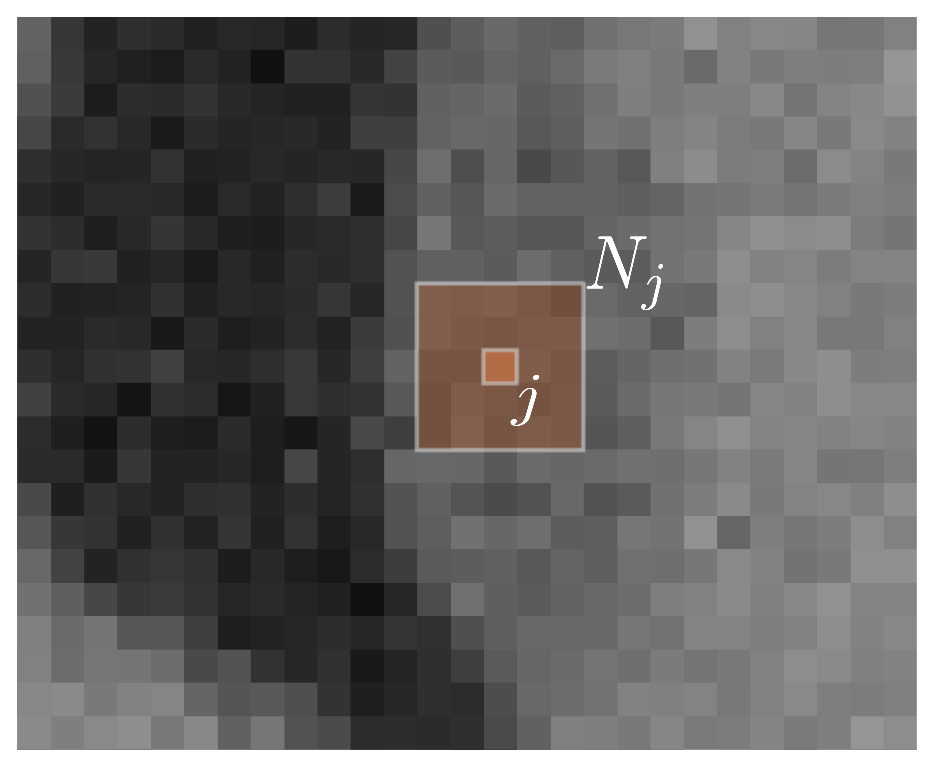
\includegraphics[height=55mm]{eps/chapitre3/Mean_Filter.eps}}
\subfigure[]{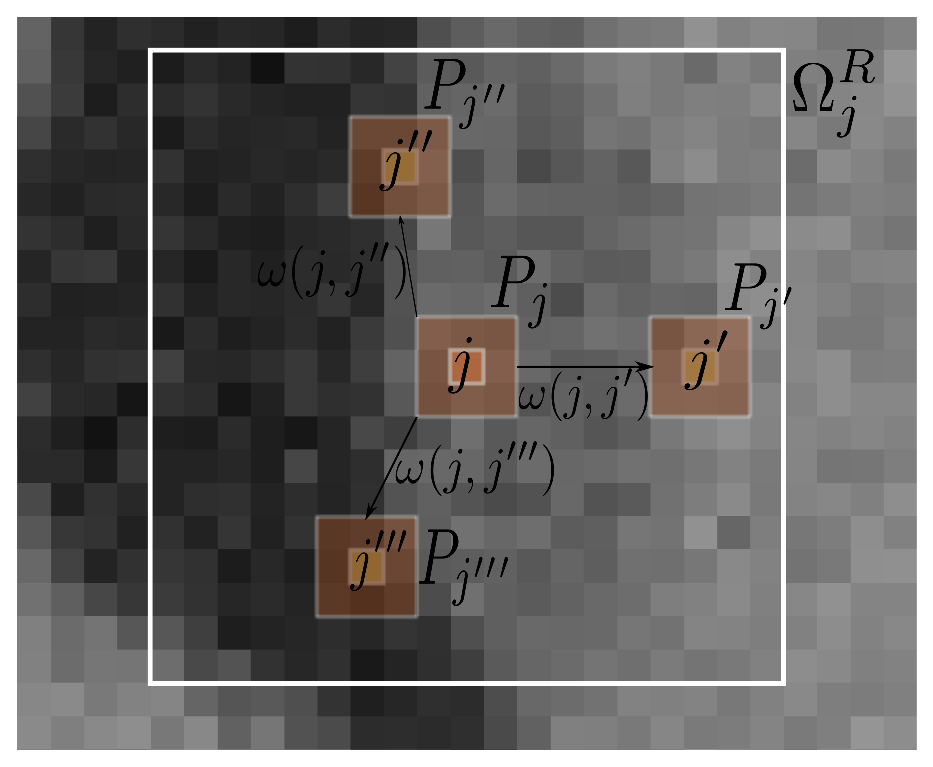
\includegraphics[height=55mm]{eps/chapitre3/NL_Mean_Filter.eps}}
\end{center}
\caption{\emph{(a) Débruitage par moyennes. L'estimation de l'intensité du voxel central est une moyenne de l'ensemble des voxels du voisinage $N_j$. (b) Débruitage par moyennes non-locales~\cite{Buades:MMS:2005}. Un poids est attribué à chaque voxel de la zone de recherche $\Omega^R_j$ selon la similarité de son patch avec celui du voxel central.}}
\label{fig:mean_filter}
\end{figure}

Avec cette définition du patch, l'estimation non-locale de l'intensité corrigée au voxel $j$ est donnée par : 
\begin{equation}
\mathbf{\hat{y}}_{j} = \frac{\sum_{l=1}^{N} K \left( \frac{\lVert P^{I}_{j} - P^{I}_{l} \rVert}{h} \right) \cdotp \mathbf{y}_{j} }{\sum_{l=1}^{N} K \left(\frac{ \lVert P^{I}_{j} - P^{I}_{l} \rVert}{h} \right)} \label{nlfcm:estimateur:complet}.
\end{equation}
Cette formulation est proche des estimateurs par noyau en statistique.
En effet, l'estimation de la valeur optimale $\mathbf{\hat{y}}_{j}$ du voxel $j$ nécessite un noyau $K(\cdotp)$ (une fonction de $\mathbb{R}$ dans $\mathbb{R}$) et une \emph{fenêtre} $h$ (régit le degré de lissage de l'estimation).
La calcul de la similarité est effectué par la comparaison entre les patchs respectifs des voxels considérés et est contrôlé par le choix de la norme $\lVert \cdotp \rVert$.
Cette formulation correspond à une moyenne pondérée des voxels sur l'ensemble du support de l'image.
% La nouveauté de cette méthode réside dans le calcul de la similarité entre les voxels, celle-ci se faisant par comparaison de leur patch. 
% La pondération entre les voxels est déduite directement de la mesure de la similarité. 
% Le choix de la fonction noyaux et du paramètre $h$ entrent alors en jeu.

Constatant que l'estimateur se présente sous la forme d'une moyenne pondérée, nous pouvons réécrire la formule \ref{nlfcm:estimateur:complet} sous la forme :
\begin{equation}
\mathbf{\hat{y}}_{j} = \sum_{l = 1}^{N}\omega_{nl}(j,l) \cdotp \mathbf{y}_{l} \label{nlfcm:estimateur:court},
\end{equation}
où $\omega_{nl}(j,l)$ est le poids non-local attribué au voxel $j'$ pour l'estimation de $\mathbf{\hat{y}}_{j}$. 
Ce terme est défini par :
\begin{equation}
\omega_{nl}(j,l) = \frac{K \left( \frac{\lVert P^{I}_{j} - P^{I}_{l} \rVert}{h} \right)}{\sum_{l=1}^{N} K \left(\frac{ \lVert P^{I}_{j} - P^{I}_{l} \rVert}{h} \right)} \label{nlfcm:poids:definition},
\end{equation}
et est donc directement liée au calcul de la similarité entre les voxels de la zone de recherche.

\subsection{Etude des paramètres régissant le comportement de l'approche non-locale}

Pour des raisons pratiques, notamment le temps d'exécution et l'efficacité du filtre, le calcul des poids non-locaux a été restreint à une zone de recherche $\Omega_{j}^{R}$ autour du voxel $j$.
Ce fait fût entériné dès l'article fondateur de \cite{Buades:MMS:2005}.
Cependant, l'influence de la taille de cette zone est un paramètre qui a peu été étudié et qui est assez difficile à évaluer.
Les différentes études concluent que cette taille est à ajuster en fonction de l'image considérée \cite{Salmon:2010}.

Plusieurs paramètres influent sur le comportement des moyennes non-locales. 
Ces paramètres peuvent être numériques, tel que le paramètre de lissage $h$, la taille des patchs $\lvert P_{j} \rvert$, ou la taille de la zone de recherche $\lvert \Omega^{R}_{j} \rvert$.
D'autres sont plus difficilement quantifiable, tels que le choix de la fonction noyau $K(\cdot)$ et de la norme $\lVert \cdot \rVert$ utilisée pour le calcul de la similarité.
De nombreux articles ont discuté les limites des moyennes non-locales et l'influence de ses paramètres.

Tout d'abord, des stratégies ont très vite été adoptées pour calculer de manière automatique le paramètre $h$ \cite{Tasdizen:ICIP:2008,Coupe:TMI:2008}. 
Par exemple, \cite{Coupe:TMI:2008} propose une méthode de calcul en montrant qu'il ne dépend que de la variance du bruit $\sigma^2$ et de la taille de la zone de recherche $\lvert \Omega^{R}_{j} \rvert$.
La fenêtre $h$ peut ainsi être évaluée par : $h = 2 \alpha \sigma^{2} \lvert \Omega^{R}_{j} \rvert$ où seul le paramètre $\alpha$ est à ajuster manuellement.
Dans la cas d'un bruit gaussien, la valeur de $\alpha$ est théoriquement à $1$ si l'estimation de la variance est correcte.

D'autres articles ont étudié l'impact de la fonction noyau et de la norme sur le débruitage. 
L'article fondateur de Buades \cite{Buades:MMS:2005} utilise un noyau gaussien $K(x) = e^{-x}$, qui est encore largement utilisé dans la littérature.
Cependant, des travaux récents \cite{Goossens:LNLA:2008, Salmon:2010} ont montré qu'un noyau à support compact \cite{Remaki:TIP:2000} est préférable.
Ces noyaux sont dérivés du noyau gaussien par une déformation de l'espace des données, le réduisant à une boule unitaire, donnant ainsi au noyau un support fini contrairement au noyau gaussien.
Cela a pour avantage d'accélérer les traitements et d'éviter les problèmes dus à la troncature du noyau (opération réalisée à cause du temps de calcul).
De manière générale, le choix d'utiliser la norme euclidienne pour le calcul de la similarité entre deux patchs a peu été remis en cause \cite{Salmon:2010}.

L'influence de la taille des patchs a été étudiée par \cite{Mairal:ECCV:2009}. 
Les principales conclusions sont que ce paramètre doit augmenter avec le niveau du bruit présent dans l'image.
De plus, le bruit peut ne pas être uniforme sur l'image et le patch doit donc être idéalement défini localement.
De plus, la nature de l'image à débruiter influe également sur l'efficacité de ce paramètre, qui est donc à fixer en fonction de l'image.

D'autres travaux ont cherché à améliorer ce filtre. 
Certains ont accéléré les traitements en partant du principe qu'un voxel appartient à plusieurs patchs différents \cite{Coupe:TMI:2008}, la valeur finale du voxel étant récupérée par un moyenne sur l'ensemble des patchs.
L'article de \cite{Kervrann:IJCV:2008} peut également être mentionné pour l'utilisation de patchs adaptatifs.
Enfin, à un niveau plus théorique, l'article de \cite{Katkovnik:IJCV:2010} assimile la première version des moyennes non-locales à une régression linéaire de niveau $0$ et l'étend à des niveaux supérieurs.

Depuis son apparition en 2005, la paradigme non-locale a été utilisé dans d'autres domaines que le débruitage d'images.
Des domaines aussi divers que la déconvolution \cite{Mignotte:PRL:2008}, les problèmes inverses \cite{Bougleux:ECCV:2008} et la reconstruction de volumes \cite{Rousseau:MIA:2010} ont bénéficié des apports de ce paradigme.
Pour en savoir plus, le lecteur est invité à lire la thèse de Salmon \cite{Salmon:2010}, portant justement sur le paradigme en lui même.

\subsection{Segmentation non-locale}

Une première utilisation des moyennes non-locales dans l'algorithme FCM a été définie par~\cite{Wang:CMIG:2008} avec une application à la segmentation cérébrale.
Cette méthodologie a été développée de manière indépendante de la notre.
Les auteurs utilisent une pondération entre information locale et information non-locale en redéfinissant la distance entre l'intensité d'un voxel et le centroïde d'une classe de la façon suivante :
\begin{equation}
D^{2}(\mathbf{y}_{j}, \mathbf{v}_{k}) = (1-\lambda_{j}) d^{2}_{l}(\mathbf{y}_{j}, \mathbf{v}_{k}) + \lambda_{j} d^{2}_{nl}(\mathbf{y}_{j}, \mathbf{v}_{k}) \label{nlfcm:wang:distance},
\end{equation}
où $D(\mathbf{y}_{j}, \mathbf{v}_{k})$ représente la distance entre l'intensité $\mathbf{y}_{j}$ du voxel $j$ et le centroïde $\mathbf{v}_k$ de la classe $k$.
Cette distance est une combinaison entre une distance locale $d_{l}(\mathbf{y}_{j}, \mathbf{v}_{k})$ et une distance non-locale $d_{nl}(\mathbf{y}_{j}, \mathbf{v}_{k})$.
Le paramètre $\lambda_{j}$ contrôle localement la proportion entre ces deux distances pour le calcul de la distance $D$.

La distance locale est calculée de la façon suivante :
\begin{equation}
d^{2}_{l}(\mathbf{y}_{j}, \mathbf{v}_{k}) = \frac{\sum_{l \in N{j}} \omega_{l} (\mathbf{y}_{j}, \mathbf{y}_{l}) \lVert \mathbf{y}_{l} - \mathbf{v}_{k} \rVert^{2}_{2}}{\sum_{l \in N{j}} \omega_{l} (\mathbf{y}_{j}, \mathbf{y}_{l})} \label{nlfcm:wang:distance:locale},
\end{equation}
où $N_{j}$ est un voisinage centré autour du voxel $j$, $\omega_{l} (\mathbf{y}_{j}, \mathbf{y}_{l}) = e^{-\frac{\lvert \mathbf{y}_{j} - \mathbf{y}_{l} \rvert}{\sigma^{2}}}$ est le poids local accordé au voxel $l$ et $\sigma^{2}$ est la variance sur $N_{j}$.
Cette distance locale représente donc une moyenne pondérée sur le voisinage $N_j$, les pondérations étant calculées à partir de la similarité entre le voxel central et ses voisins (similarité voxel à voxel et non similarité des patchs).

La distance non-locale est calculée de la façon suivante : 
\begin{equation}
d^{2}_{nl}(\mathbf{y}_{j}, \mathbf{v}_{k}) = \sum_{j' = 1}^{N}\omega_{nl}(j,j') \lVert \mathbf{y}_{j'} - \mathbf{v}_{k} \rVert^{2}_{2}.
\end{equation}
% En pratique, ce calcul de la distance non-locale est limité à une zone de recherche $\Omega^{R}_{j}$ centrée autour du voxel $j$.
Le paramètre $\lambda_{j}$ est calculé automatiquement en tenant compte de la similarité globale du patch $P^{I}_{j}$ au sein de $\Omega^{R}_{j}$. 
Plus il y a de voxels similaires au voxel central au sein de la zone de recherche $\Omega^R_j$, plus le poids de la distance non-locale dans le calcul de la distance générale sera important.
L'idée sous-jacente est qu'il existe des parties de l'image présentant peu de similarité entre les voxels (par exemple, dans une IRM cérébrale, autour des sillons cérébraux) où il est plus efficace de prendre en compte une similarité entre les voxels directement plutôt qu'entre les patchs.

% Nous montrerons que la correction du bruit présent dans une image ne nécessite pas de définir une telle distance, mais qu'il suffit d'incorporer les moyennes non-locales au sein du terme de régularisation de FCM pour obtenir une correction efficace.

\section{FCM non-local}
\label{sec:nlfcm}

Nous présentons dans cette section une amélioration de l'algorithme FCM prenant en compte les moyennes non-locales au sein du terme du terme d'attache aux données de manière à améliorer la prise en compte du biais en intensité et au sein du terme de régularisation afin d'améliorer la correction du bruit.
Dans la suite du manuscrit, l'implémentation des moyennes non-locales utilise le noyau gaussien $K(x) = e^{-x}$ et la norme euclidienne pour le calcul des similarités. 
L'estimation de la fenêtre $h$ est inspiré de \cite{Coupe:TMI:2008}, laissant un paramètre $\alpha$ à évaluer.

\subsection{Terme d'attache aux données (NL-FCM)}
\label{subsec:nl:dd}

Comme précisé dans la section \ref{subsec:fcm:def}, l'algorithme FCM considère que les centroïdes des classes sont invariants au sein de l'espace de l'image, le rendant sensible à l'inhomogénéité des intensités.
Nous avons vu à la section~\ref{subsec:fcm:bias} qu'il est alors nécessaire de définir un modèle du biais explicite de manière à en prévenir les effets sur la segmentation.
Cependant, de nombreuses hypothèses doivent être faites pour pouvoir estimer ce biais, notamment sur sa nature multiplicative, la nature lente des variations d'intensité (valable que pour les inhomogénéité dues à l'imageur), la modélisation du biais lui même (polynomiales, B-Splines, \ldots{}) ou encore la définition d'un champ de biais unique ou d'un champ par tissu.

Une approche locale de la segmentation est une alternative intéressante car elle permet une estimation des modèles d'intensité dans des sous-volumes du volume complet sans avoir recours à une estimation explicite du biais.
Une même intensité peut donc être étiqueter différemment selon l'estimation locale du modèle.
La taille des sous-volumes est cependant cruciale car un sous-volume trop important sera sensible à l'inhomogénéité tandis qu'un volume trop petit risque de conduire à une mauvaise évaluation du modèle d'intensité local. 
Dans le cas de l'IRM cérébrale, une fenêtre trop petite peut, par exemple, conduire à une mauvaise évaluation dans des zones de grande concentration de matière blanche.
En effet, trop peu de voxels représentant la matière grise ou le LCR (voir aucun) seraient alors pris en compte pour permettre une estimation fiable des centroïdes des classes représentant ces tissus. 
Or l'algorithme FCM reposant sur l'estimation de ces centroïdes, cela conduirait à une classification finale faussée.

Définie dans le cadre de FCM, cette notion de modèle local se traduit par la minimisation de la fonction d'énergie suivante : 
\begin{equation}
J = \sum_{j \in \Omega} \sum_{k=1}^{C} u^{q}_{jk} \lVert \mathbf{y}_{j} - \mathbf{v}_{jk} \rVert_{2}^{2}. \label{eq:fcm:local}
\end{equation}
La différence entre cette fonction coût et celle de l'algorithme FCM classique réside dans l'introduction de centroïdes locaux $\mathbf{v}_{jk}$ fournissant une évaluation du modèle d'intensité au voxel $j$, le problème de cette évaluation restant ouvert.
Des approches par recouvrement de sous-volumes ont été définies telle que celle de \cite{Zhu:NeuroImage:2003} comportant une étape de classification par FCM proprement dite, puis une étape de fusion de l'information.
De même, \cite{Scherrer:TMI:2009} introduit des modèles markoviens locaux par la division de l'image en sous-volumes et estime ces modèles en coopération avec les modèles voisins afin d'assurer la cohérence de l'ensemble de la segmentation.
Ces deux approches se positionnent dans une optique de fusion d'information pour résoudre le problème de la segmentation.
% Cependant, ce genre d'approche peut-être vu comme un déplacement du problème de l'évaluation d'un modèle vers celui de la fusion de plusieurs modèles.

A notre connaissance, aucune méthode ne permet la prise en compte des modèles voisins sans une approche de fusion de l'information.
Cependant, l'approche non-locale permet de mettre en \oe uvre une pondération entre les différents voxels de l'image en fonction de la similarité de leur patch.
En faisant l'hypothèse que deux voxels dont les patchs sont similaires font parti du même tissus, il est possible d'utiliser ces pondérations pour prendre en compte les modèles voisins (c'est-à-dire l'estimation des moyennes locales aux voxels voisins) pour diminuer le risque qu’entraine une mauvaise évaluation des moyennes locales.
Un terme d'attache aux données non-local est alors défini de la façon suivante :
\begin{equation}
J_{NL-FCM} = \sum_{j \in \Omega} \sum_{k=1}^{C} u_{jk}^{q} \sum_{l \in \Omega^{R_d}_{j}} \omega_{nl}(j, l) \Vert \mathbf{y}_{j} - \mathbf{v}_{lk} \Vert_2^{2} \label{eq:nlfcm:dd}.
\end{equation}
Ce terme d'attache aux données doit permettre une meilleure robustesse de la segmentation en cas de mauvaise évaluation de certains modèles locaux.

Deux différences sont notables par rapport à la définition standard de FCM (donnée par l'équation \ref{eq:fcm}).
La première a déjà été évoquée et consiste à remplacer le terme global des centroïdes $\mathbf{v}_{k}$ dans FCM par un terme local $\mathbf{v}_{jk}$ de manière à bénéficier d'une évaluation locale du modèle d'intensité.
Ces centroïdes locaux sont calculés à partir d'un sous-volume $M_j$ centré autour du voxel $j$ et dont l'influence de la taille est discutée plus loin.
La deuxième différence est que chaque modèle inclus dans la zone de recherche $\Omega^{R_d}_{j}$ va avoir une influence sur la classification finale du voxel $j$.
Un modèle étant défini pour chaque voxel de l'image, cette proportion est donc contrôlée par le poids non-local $\omega_{nl}(j,j')$ traduisant la similarité entre le voxel $j$ et chacun des voxels $j'$ inclus dans la zone de recherche.  

\subsection{Terme de régularisation (NL-Reg)}
\label{subsec:nl:reg}

Dans les précédents travaux, le terme de régularisation s'apparente la plupart du temps à l'expression d'un filtrage médian ou par moyenne pour lisser la segmentation.
Plusieurs articles ont introduits différentes stratégies permettant de prendre en compte la similarité entre les voxels (introduisant ainsi une pondération entre les voxels d'un même voisinage), mais cette prise en compte nécessite le calcul de plusieurs variables additionnelles ou la définition d'une image intermédiaire.

Les moyennes non-locales sont particulièrement intéressantes dans cette situation, car elles fournissent les outils nécessaire à une pondération relativement aisée des voxels d'intêret au sein de la zone de recherche.
Le rôle de poids non-locaux est donc de sélectionner les voxels les plus pertinents au sein de la zone de recherche pour effectuer la régularisation en fonction de leur degré de similarité avec le voxel courant.
L'hypothèse que nous faisons est que si deux voxels sont similaires, alors ils appartiennent au même tissu.
L'objectif est d'obtenir une régularisation plus lisse de façon adaptative et naturelle.

Le terme de régularisation défini dans cette section s'inspire de celui de~\cite{Pham:CVIU:2001} (dont la définition est donnée par l'équation \ref{eq:rfcm}), régularisant la proportion d'une classe au sein d'un voxel en prenant en compte la proportion des autres classes dans le voisinage.
Le terme de régularisation non-local est exprimé de la façon suivante :
\begin{equation}
J_{NL\textrm{-}Reg} =
\frac{\beta}{2} \sum_{j \in \Omega} \sum_{k=1}^{C} u_{jk}^{q} \sum_{j' \in \Omega^{R_{r}}_{j}} \omega_{nl}(j, j') \sum_{l \in L_{k}} u_{j'l}^{q} \label{eq:nlfcm:reg}.
\end{equation}

Rappelons que $L_{k}=[\![1,C]\!]\setminus \{k\} = \{1, \ldots, k-1, k+1, \ldots, C\}$ et représente donc l'ensemble des classes exceptée la classe dont on effectue la régularisation et $\Omega^{R_{r}}_{j}$ représente la zone de recherche centrée autour du voxel $j$ destinée à calculer les poids non-locaux pour la régularisation.
Le paramètre $\beta$ contrôle les poids respectifs entre le terme de régularisation et le terme d'attache aux données au sein de la fonction d'énergie.

\subsection{Algorithme non-local complet (NL-R-FCM)}

L'association des deux termes non locaux donne un algorithme de segmentation non local complet permettant de prendre en compte l'inhomogénéité et le bruit de l'image. 
La fonction d'énergie devient donc : 
\begin{equation}
\begin{split}
J_{NL\textrm{-}R\textrm{-}FCM} =\\
\sum_{j \in \Omega} \sum_{k=1}^{C} \sum_{j' \in \Omega^{R_d}_{j}} \omega_{nl}(j, j') u_{jk}^{q} \Vert \mathbf{y}_{j} - \mathbf{v}_{j'k} \Vert_2^{2} \\
+ \frac{\beta}{2} \sum_{j \in \Omega} \sum_{k=1}^{C} u_{jk}^{q} \sum_{j'' \in \Omega^{R_{r}}_{j}} \omega_{nl}(j, j'') \sum_{l \in L_{k}} u_{j'l}^{q} \label{eq:nlfcm:reg}.
\end{split}
\end{equation}

Il est important de noter que les poids $\omega_{nl}(\cdot,\cdot)$ présents dans le terme d'attache aux données et le terme de régularisation sont distincts et ne sont pas utilisés dans le même but.
De même, les zone de recherche $\Omega^{R_d}_{j}$ et $\Omega^{R_r}_{j}$ n'ont pas nécessairement la même taille.

Les différentes étapes permettant de minimiser la fonction d'énergie du FCM non-local sont les suivantes : 
\begin{enumerate}
\item Calculer les poids non-locaux $\omega_{nl}$ pour le terme d'attache aux données et le terme de régularisation.
\item Calculer les centroïdes $\mathbf{v}_{jk}$ pour tout $(j,k) \in [\![ 1,C ]\!]\times \Omega$ (évaluation initiale).
\item Calculer $u_{jk}$ pour tout $(j,k) \in [\![ 1,C ]\!]\times \Omega$ (évaluation initiale).
\item Répéter jusqu'à un minimum local de la fonction d'énergie : 
\begin{itemize}
\item Recalculer $\mathbf{v}_{jk}$ pour tout $(j,k) \in [\![ 1,C ]\!]\times \Omega$.
\item Recalculer $u_{jk}$ pour tout $(j,k) \in [\![ 1,C ]\!]\times \Omega$.
\end{itemize}

\end{enumerate}

La donnée d'entrée de l'algorithme est l'image à segmenter (fournissant $\Omega$ et les valeurs $\mathbf{y}$).
Les paramètres déterminant son comportement sont : $C$ (le nombre de classes), $\beta$ (qui contrôle le rapport entre le terme d'attache aux données et le terme de régularisation), la taille de la zone de recherche pour le calcul des poids non-locaux destinés à la régularisation $\Omega^{R_r}_j$, la taille de la zone de recherche pour le calcul des poids non-locaux destinés au terme d'attache aux données $\Omega^{R_d}_j$, la taille des sous-volume $M_j$ permettant l'estimation des modèles locaux et le paramètre de lissage $\alpha$.

\section{Validations}
\label{sec:nlfcm:validations}

Les expériences permettant la validation des FCM non-locaux sont menées tout d'abord sur des images simulées fournies par la base BrainWeb \cite{Cocosco:FMHB:1997, Kwann:VBC:1996}, puis sur des cas réels fournis par la base IBSR (\emph{Internet Brain Segmentation Repository}).

Considérant tout d'abord la base BrainWeb, trois séries d'expériences sont menées de manière à déterminer le comportement de l'algorithme FCM non-local et d'évaluer ses performances par rapport à d'autres méthodes :
\begin{enumerate}
        \item Évaluation du terme d'attache aux données non-locale en utilisant des images ayant 20~\% d'inhomogénéité en intensité (voir la section~\ref{sec:brainweb:nlData}).
        \item \'Evaluation du terme de régularisation non-locale en utilisant des images ayant différents niveaux de bruit ricien (voir la section~\ref{sec:brainweb:nlReg}).
        \item Évaluation de l'algorithme non-local complet en utilisant des images ayant à la fois 20~\% d'inhomogénéité en intensité et différents niveaux de bruit (voir la section~\ref{sec:brainweb:nlAll}).
\end{enumerate}
Par la suite, l'algorithme FCM non-local complet est appliqué à l'ensemble de la base IBSR et comparé à d'autres méthodologies.

L'évaluation des performances des différents algorithmes est faite par comparaison de la segmentation simulée avec la vérité terrain fournie par les bases d'images respectives.
La qualité de la segmentation est mesurée par le calcul de l'indice de similarité Dice : 
$$
Dice = \frac{2\cdotp VP}{2\cdotp VP + FP + FN},
$$
où $VP$ est le nombre de vrais positifs, $FP$ le nombre de faux positifs et $FN$ le nombre de faux négatifs.
Cet indice calcule un taux de recouvrement entre la vérité terrain et la segmentation automatique.

De plus, l'évaluation inclue à chaque étape une comparaison avec d'autres méthodes de classification reposant sur les champs et chaînes de Markov.
Ces méthodes sont : 
\begin{itemize}
        \item SPM5 de Ashburner \emph{et al.}~\cite{Ashburner:NeuroImage:2005},
        \item EMS de Van Leemput \emph{et al.}~\cite{VanLeemput2:TMI:1999},
        \item HMC de Bricq \emph{et al.}~\cite{Bricq:MIA:2008}.
\end{itemize}
Rappellons que les méthodes SPM5 et EMS incluent une correction du biais, ainsi qu'une classification avec régularisation par champs de Markov.
Enfin, HMC inclue une correction du biais, tout en s'appuyant sur les chaînes de Markov pour la régularisation, chose rendue possible par un parcours fractal d'Hilbert-Peano permettant de conserver au mieux les informations de voisinage.

% \subsection{Outils de validation}
% 
% \begin{table}[!ht]
% 
% \begin{center}
% 
% \begin{tabular}{|c|c|}
% \hline
% $VP$ & Vrais Positif\\
% \hline
% $FP$ & Faux Positif\\
% \hline
% $VN$ & Vrais Negatif\\
% \hline
% $FN$ & Faux Negatif\\
% \hline
% \end{tabular}
% \caption{Abrévations utilisées pour la validation. \label{table:validation:abr}}
% \end{center}
% 
% \end{table}
% 
% Pour évaluer la performance de notre algorithme, la qualité de la segmentation est jugée par rapport à plusieurs index couramment utilisés dans la littérature.
% Une table des abrévations est fournie par la table~\ref{table:validation:abr}.
% 
% Ces indices sont :
% \begin{itemize}
% 
% \item la sensibilité (\emph{True Positive Fraction}) :
% $$
% Sen = \frac{VP}{VP + FN},
% $$
% 
% \item la spécificité :
% $$
% Spe = \frac{VN}{VN + FP},
% $$
% 
% \item la similarité (appelée aussi coefficient de Dice) : 
% $$
% Dice = \frac{2\cdotp VP}{2\cdotp VP + FP + FN}.
% $$
% \end{itemize}
% 
% Dans la suite du manuscrit, ces estimateurs seront donnés en pourcentage.


\subsection{Brainweb}
\label{subsec:brainweb}

Le dépôt de BrainWeb~\footnote{\url{http://www.bic.mni.mcgill.ca/brainweb/}} permet de simuler des IRM cérébrales avec différents niveaux de bruit et d'inhomogénéité et fournit la vérité terrain correspondante, permettant de comparer différents algorithmes de segmentation.
% La connaissance de la vérité terrain permet de comparer différents algorithmes de segmentation.
Les images fournies par la base sont issues de 27 acquisitions réalisées sur un même individu.
Elles sont ensuite moyennées pour construire le volume initial auquel sont ensuite appliqués divers traitements pour créer le fantôme~\cite{Collins:TMI:1998}.
Les images utilisées sont de taille $181\times181\times217$ avec des voxels isotropes de $1$ mm de côté.
Le bruit est de type ricien d'un niveau allant de $0$ à $9$~\%.

\subsubsection{Évaluation du terme d'attache aux données}
\label{sec:brainweb:nlData}

L'algorithme est initialisé grâce à un atlas fourni avec la base BrainWeb.
Il permet d'initialiser de manière fiable les moyennes locales avant le lancement de NL-FCM proprement dit et fournit une première estimation de la classification des tissus.

\paragraph*{Etude des paramètres}

Les paramètres étudiés sont la taille de la zone de recherche $\lvert \Omega^{R_{d}}_{j} \rvert$ pour le calcul des poids non-locaux et la taille du voisinage $M_j$ pour le calcul des centroïdes locaux.
On pose $n_j$ et $m_j$ tels que : $\lvert \Omega^{R_{d}}_{j} \rvert = (2 \cdot n_j + 1)^{3}$ et $\lvert M_{j} \rvert = (2 \cdot m_j + 1)^{3}$.

\begin{figure}[!thbp]

        \begin{center}
	\subfigure[]{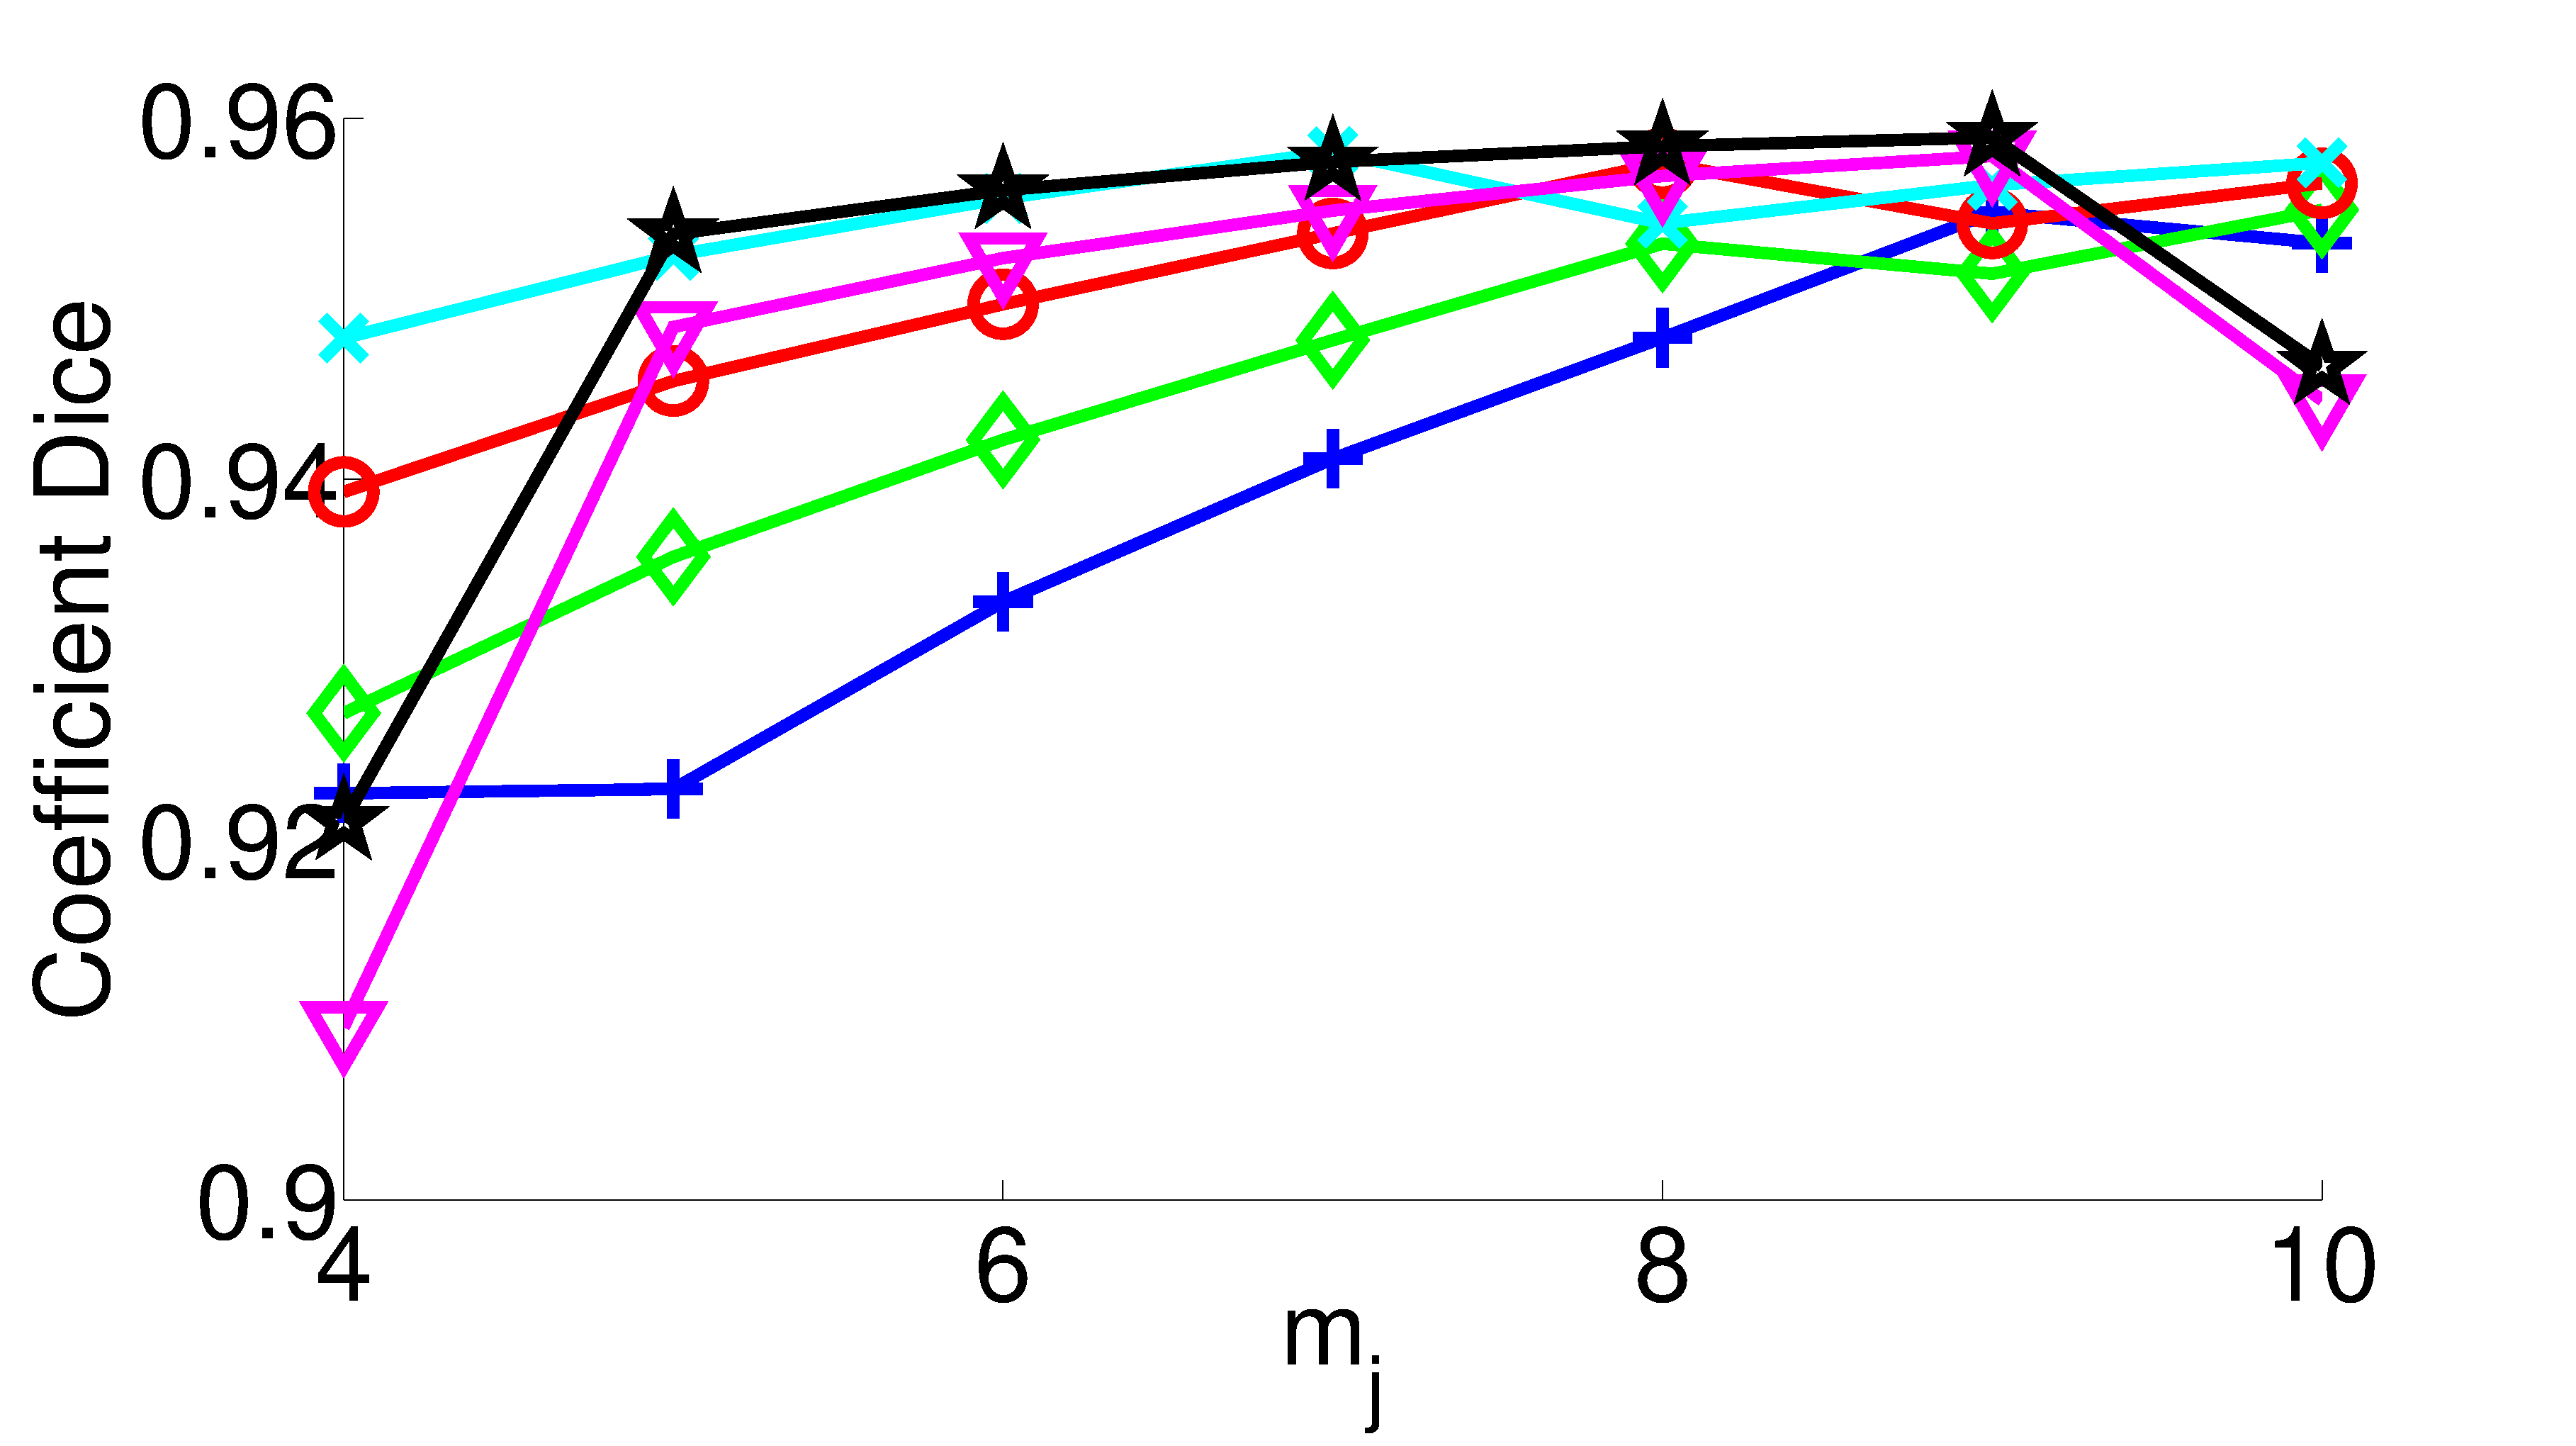
\includegraphics[height=38mm]{eps/chapitre3/Brainweb_Bias_Couple_GM.eps}}
	\subfigure[]{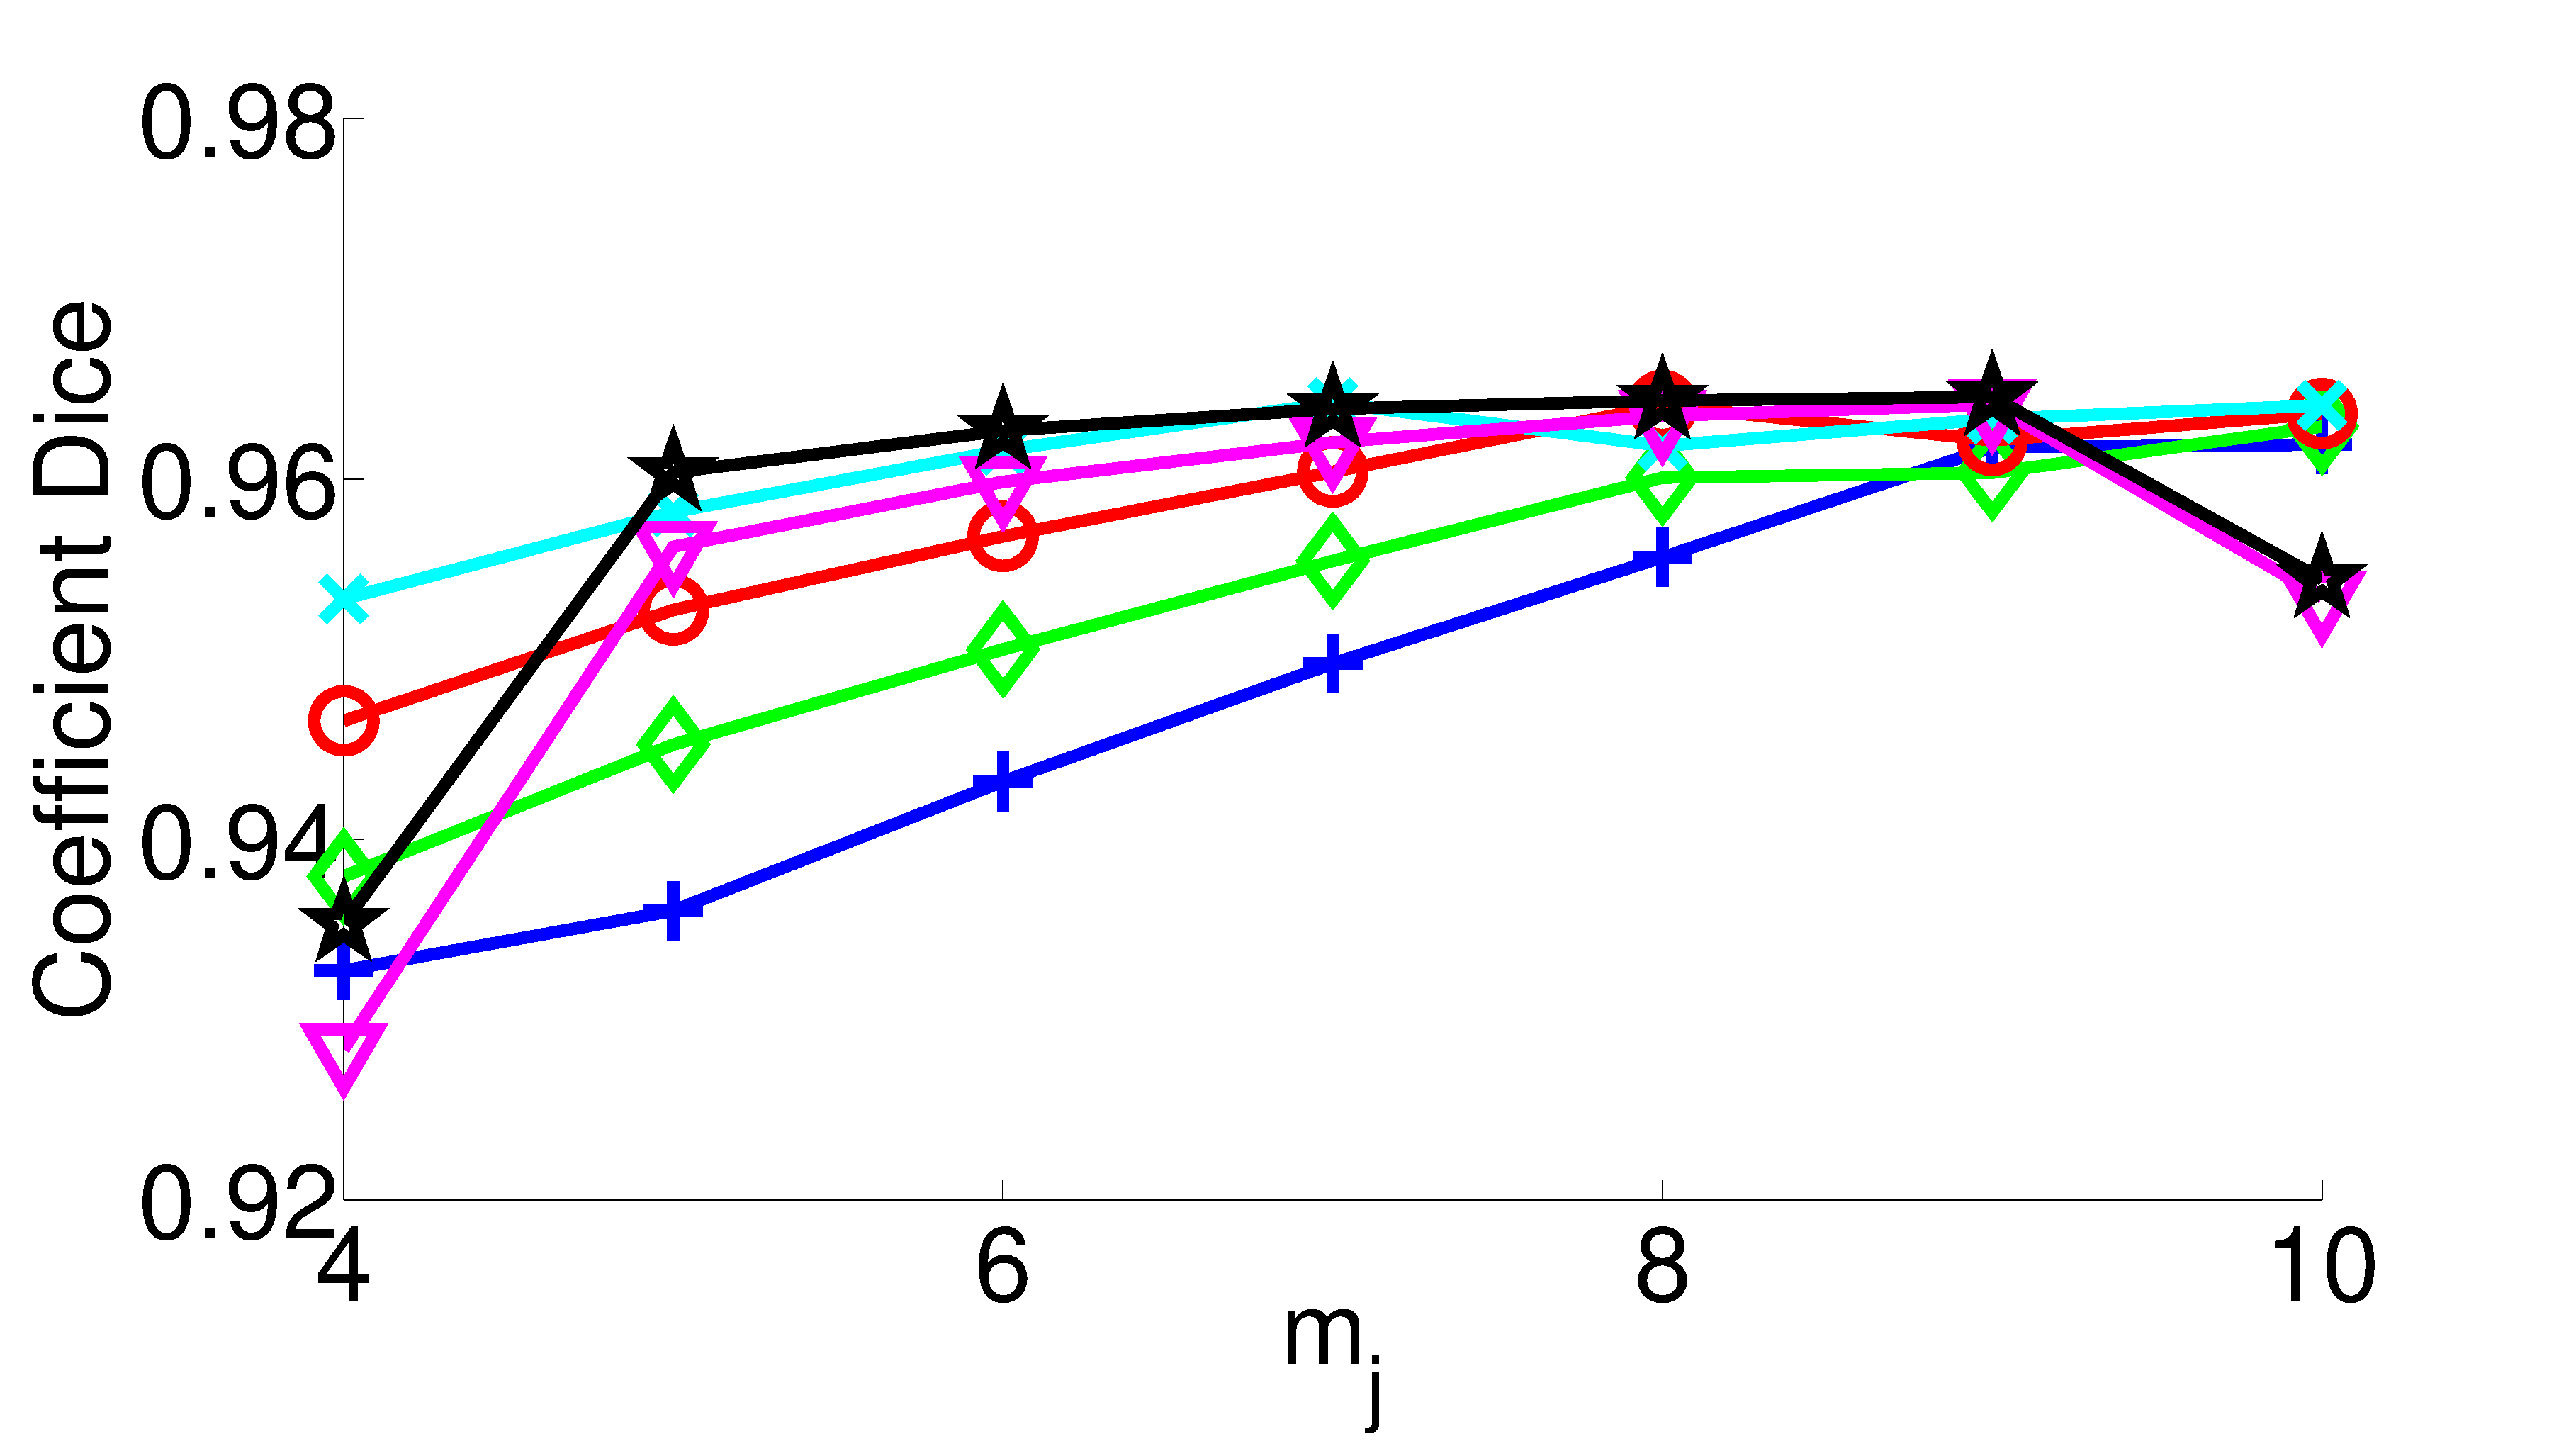
\includegraphics[height=38mm]{eps/chapitre3/Brainweb_Bias_Couple_WM.eps}}
        \end{center}

        \caption{\emph{Influence des paramètres $M_j$ et $\Omega^{R_d}_j$ du terme d'attache aux données non-locale. L'accroissement de la zone de recherche $\Omega^{R_d}_{j}$ permet de compenser les éventuelles mauvaises évaluation du modèle dues à des sous-volumes $M_j$ trop réduits. (a) Coefficient Dice pour la matière grise. (b) Coefficient Dice pour la matière blanche. $n_j = 4$ : $+$, $n_j = 5$ : $\diamond$, $n_j = 6$ : $\circ$, $n_j = 7$ : $\times$, $n_j = 8$ : $\bigtriangledown$, $n_j = 9$ : $\star$.}}

        \label{FIG:PARAM:BRAINWEB:BIAS}

\end{figure}

La figure~\ref{FIG:PARAM:BRAINWEB:BIAS} montre les résultats avec différents sous-volumes et différentes zone de recherche.
Comme attendu, à sous-volume égal, l'accroissement de la taille de zone de recherche permet d'obtenir une meilleure segmentation par la prise en compte des modèles voisins et la pondération en résultant.
Les paramètres finaux choisis pour la suite des expérience sont un compromis entre la performance et le temps de calcul de l'algorithme.
Ils sont fixés à : $(n_j, m_j) = (8, 8)$ (voir la figure~\ref{FIG:PARAM:BRAINWEB:BIAS}).

\paragraph*{Comparaison à d'autres méthodologies}

Ce terme d'attache aux données non-locale a été comparé à la version classique de l'algorithme FCM ainsi qu'à SPM5, EMS et HMC. 
La table~\ref{TAB:DICE:BRAINWEB:BIAS} récapitule les taux de recouvrement obtenus avec les différentes méthodes de segmentation.
La figure~\ref{FIG:VIEW:BRAINWEB:BIAS} illustre les performances du terme d'attache aux données non-locale dans un environnement présentant un biais en intensité.

\begin{table}[!htb]
\begin{center}
\begin{tabular}{|l | *{2}{c|}}
	\hline
	Méthodes &  Matière grise & Matière blanche \\
	\hline
	SPM5 & 91.4 & 91.3 \\
	EMS & 83.7 & 86.9\\
	HMC & 94.0 & 95.9\\
	FCM & 69.2 & 75.83\\
	NL-FCM & \fbox{95.68} & \fbox{96.35}\\
	\hline 
\end{tabular}
% \vspace{2mm}
\caption{\emph{Application de différentes segmentations à une image pondérée en T1 présentant un biais en intensité de 20~\%. Comparaison des différents coefficient Dice pour la segmentation de la matière grise et de la matière blanche. Paramètres pour NL-FCM : $n_j = 8$ et $m_j = 8$. \label{TAB:DICE:BRAINWEB:BIAS}}}
\end{center}
\end{table}

\begin{figure}[!thbp]

        \begin{center}
	\subfigure[]{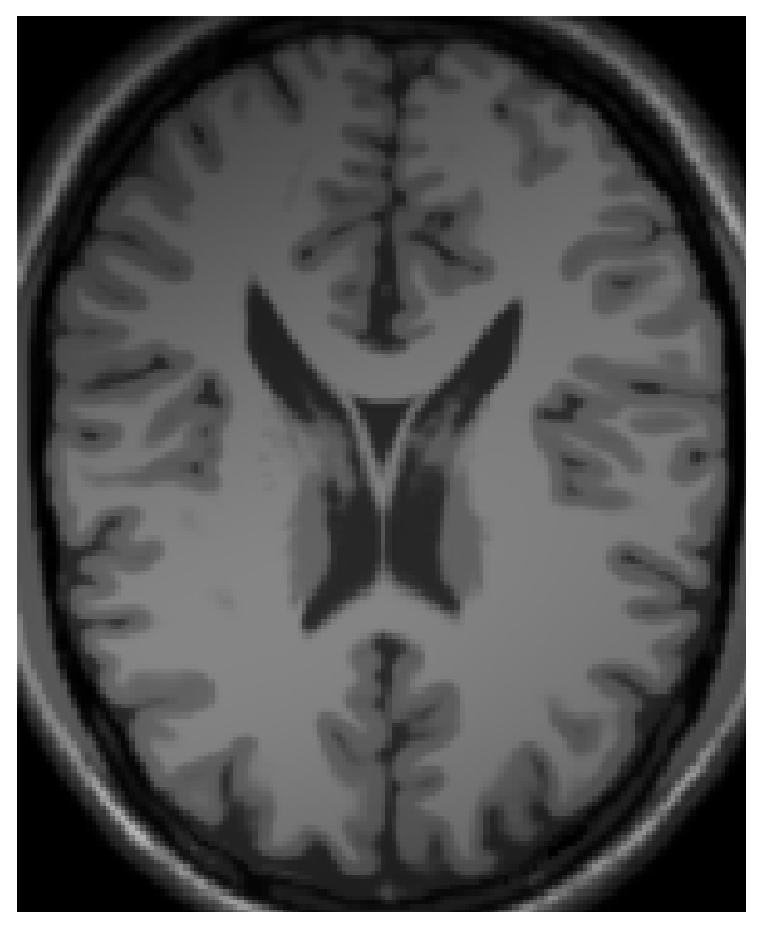
\includegraphics[height=41mm]{eps/chapitre3/Brainweb_Bias_T1.eps}}
	\subfigure[]{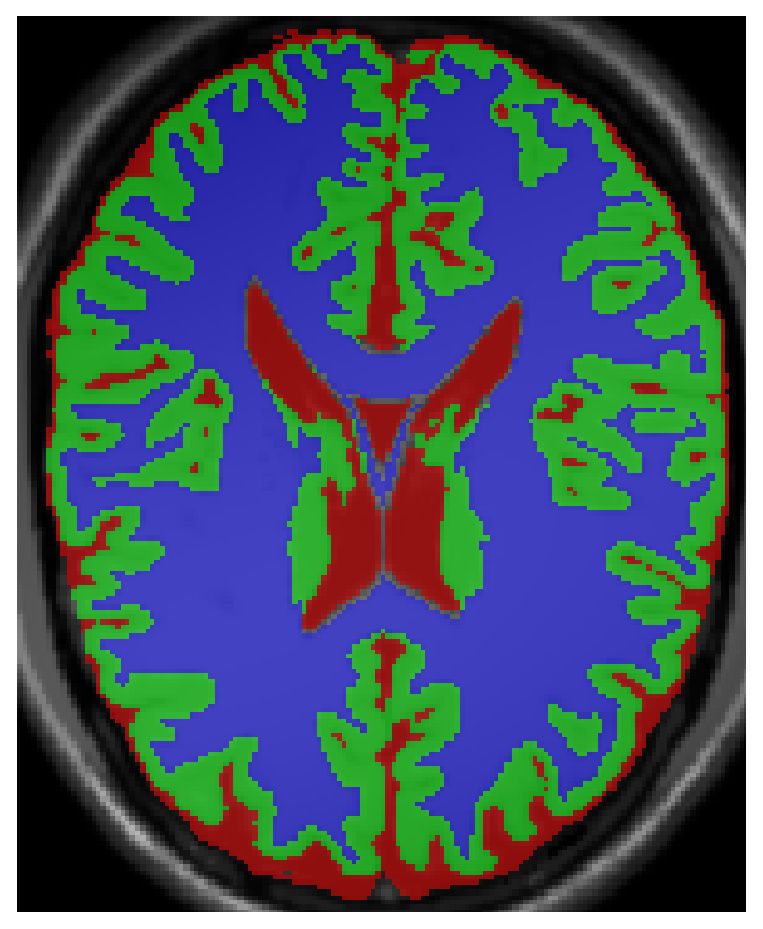
\includegraphics[height=41mm]{eps/chapitre3/Brainweb_Bias_truth.eps}}
	\subfigure[]{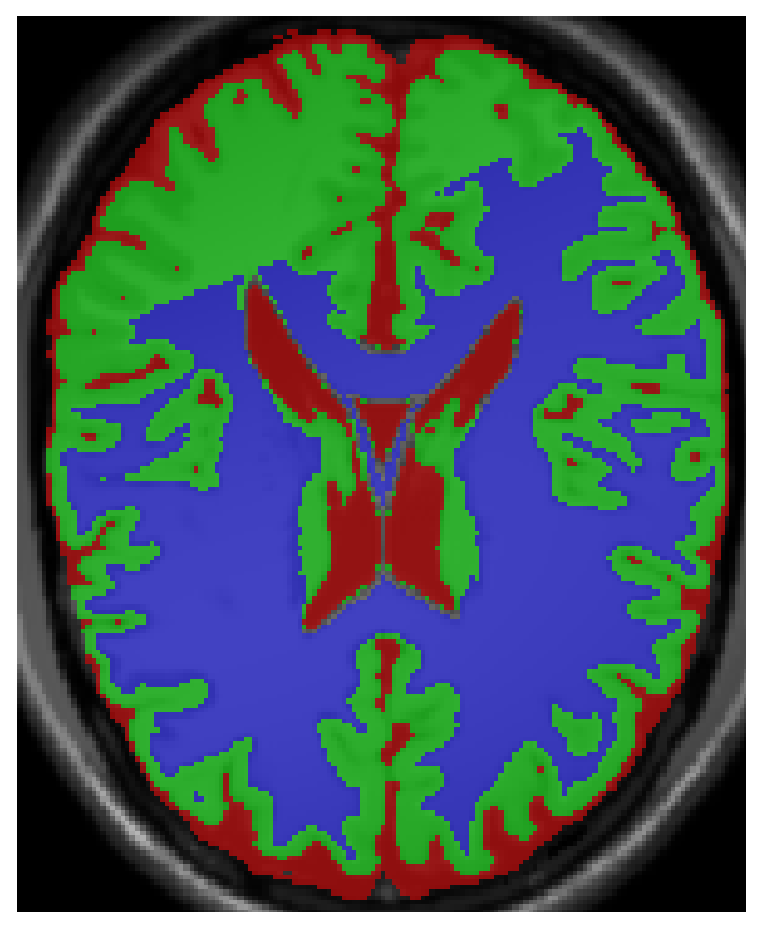
\includegraphics[height=41mm]{eps/chapitre3/Brainweb_Bias_classicfcm.eps}}
	\subfigure[]{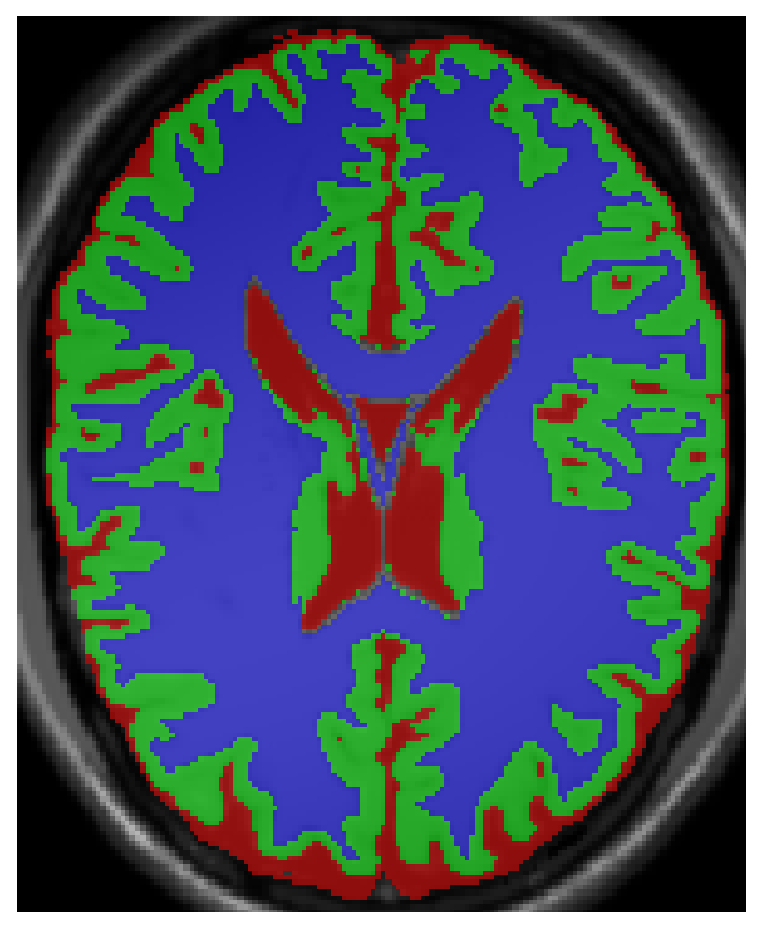
\includegraphics[height=41mm]{eps/chapitre3/Brainweb_Bias_nlfcm.eps}}
        \end{center}

        \caption{\emph{Résultats de la segmentation d'une image T1 présentant un biais en intensité. (a) Coupe d'une image T1. (b) Vérité terrain. (c) Segmentation par FCM classique. (d) Segmentation par FCM non-local.}}

        \label{FIG:VIEW:BRAINWEB:BIAS}

\end{figure}

Nous pouvons observer que l'algorithme FCM non local permet une correction du biais en intensité similaire à la meilleure méthode fondée sur les chaînes de Markov et améliore nettement les performance de l'algorithme FCM malgré l'absence d'une évaluation explicite du biais en intensité.
Le temps de calcul est cependant très pénalisant.
En effet, environ huit heures de calcul sur un PC standard sont nécessaires pour segmenter une image.

\subsubsection{Evaluation du terme de régularisation}
\label{sec:brainweb:nlReg}

L'algorithme NL-Reg est initialisé par un algorithme des K-Moyennes de manière à obtenir une première estimation de la distribution en intensité et les cartes de probabilité sont initialisées à $\frac{1}{C}$ ($C$ étant le nombre de classes recherchées).
Dans un premier temps, des tests sont réalisés sur une image bruitée à $5$~\% afin d'évaluer l'influence des paramètres non-locaux sur la segmentation.
Enfin, différentes segmentations sont réalisées avec les paramètres optimaux obtenus pour étudier le comportement du terme de régularisation non-local en fonction du bruit.

\paragraph*{Influence des paramètres non-locaux}

\begin{figure}[!thbp]

        \begin{center}
	\subfigure[]{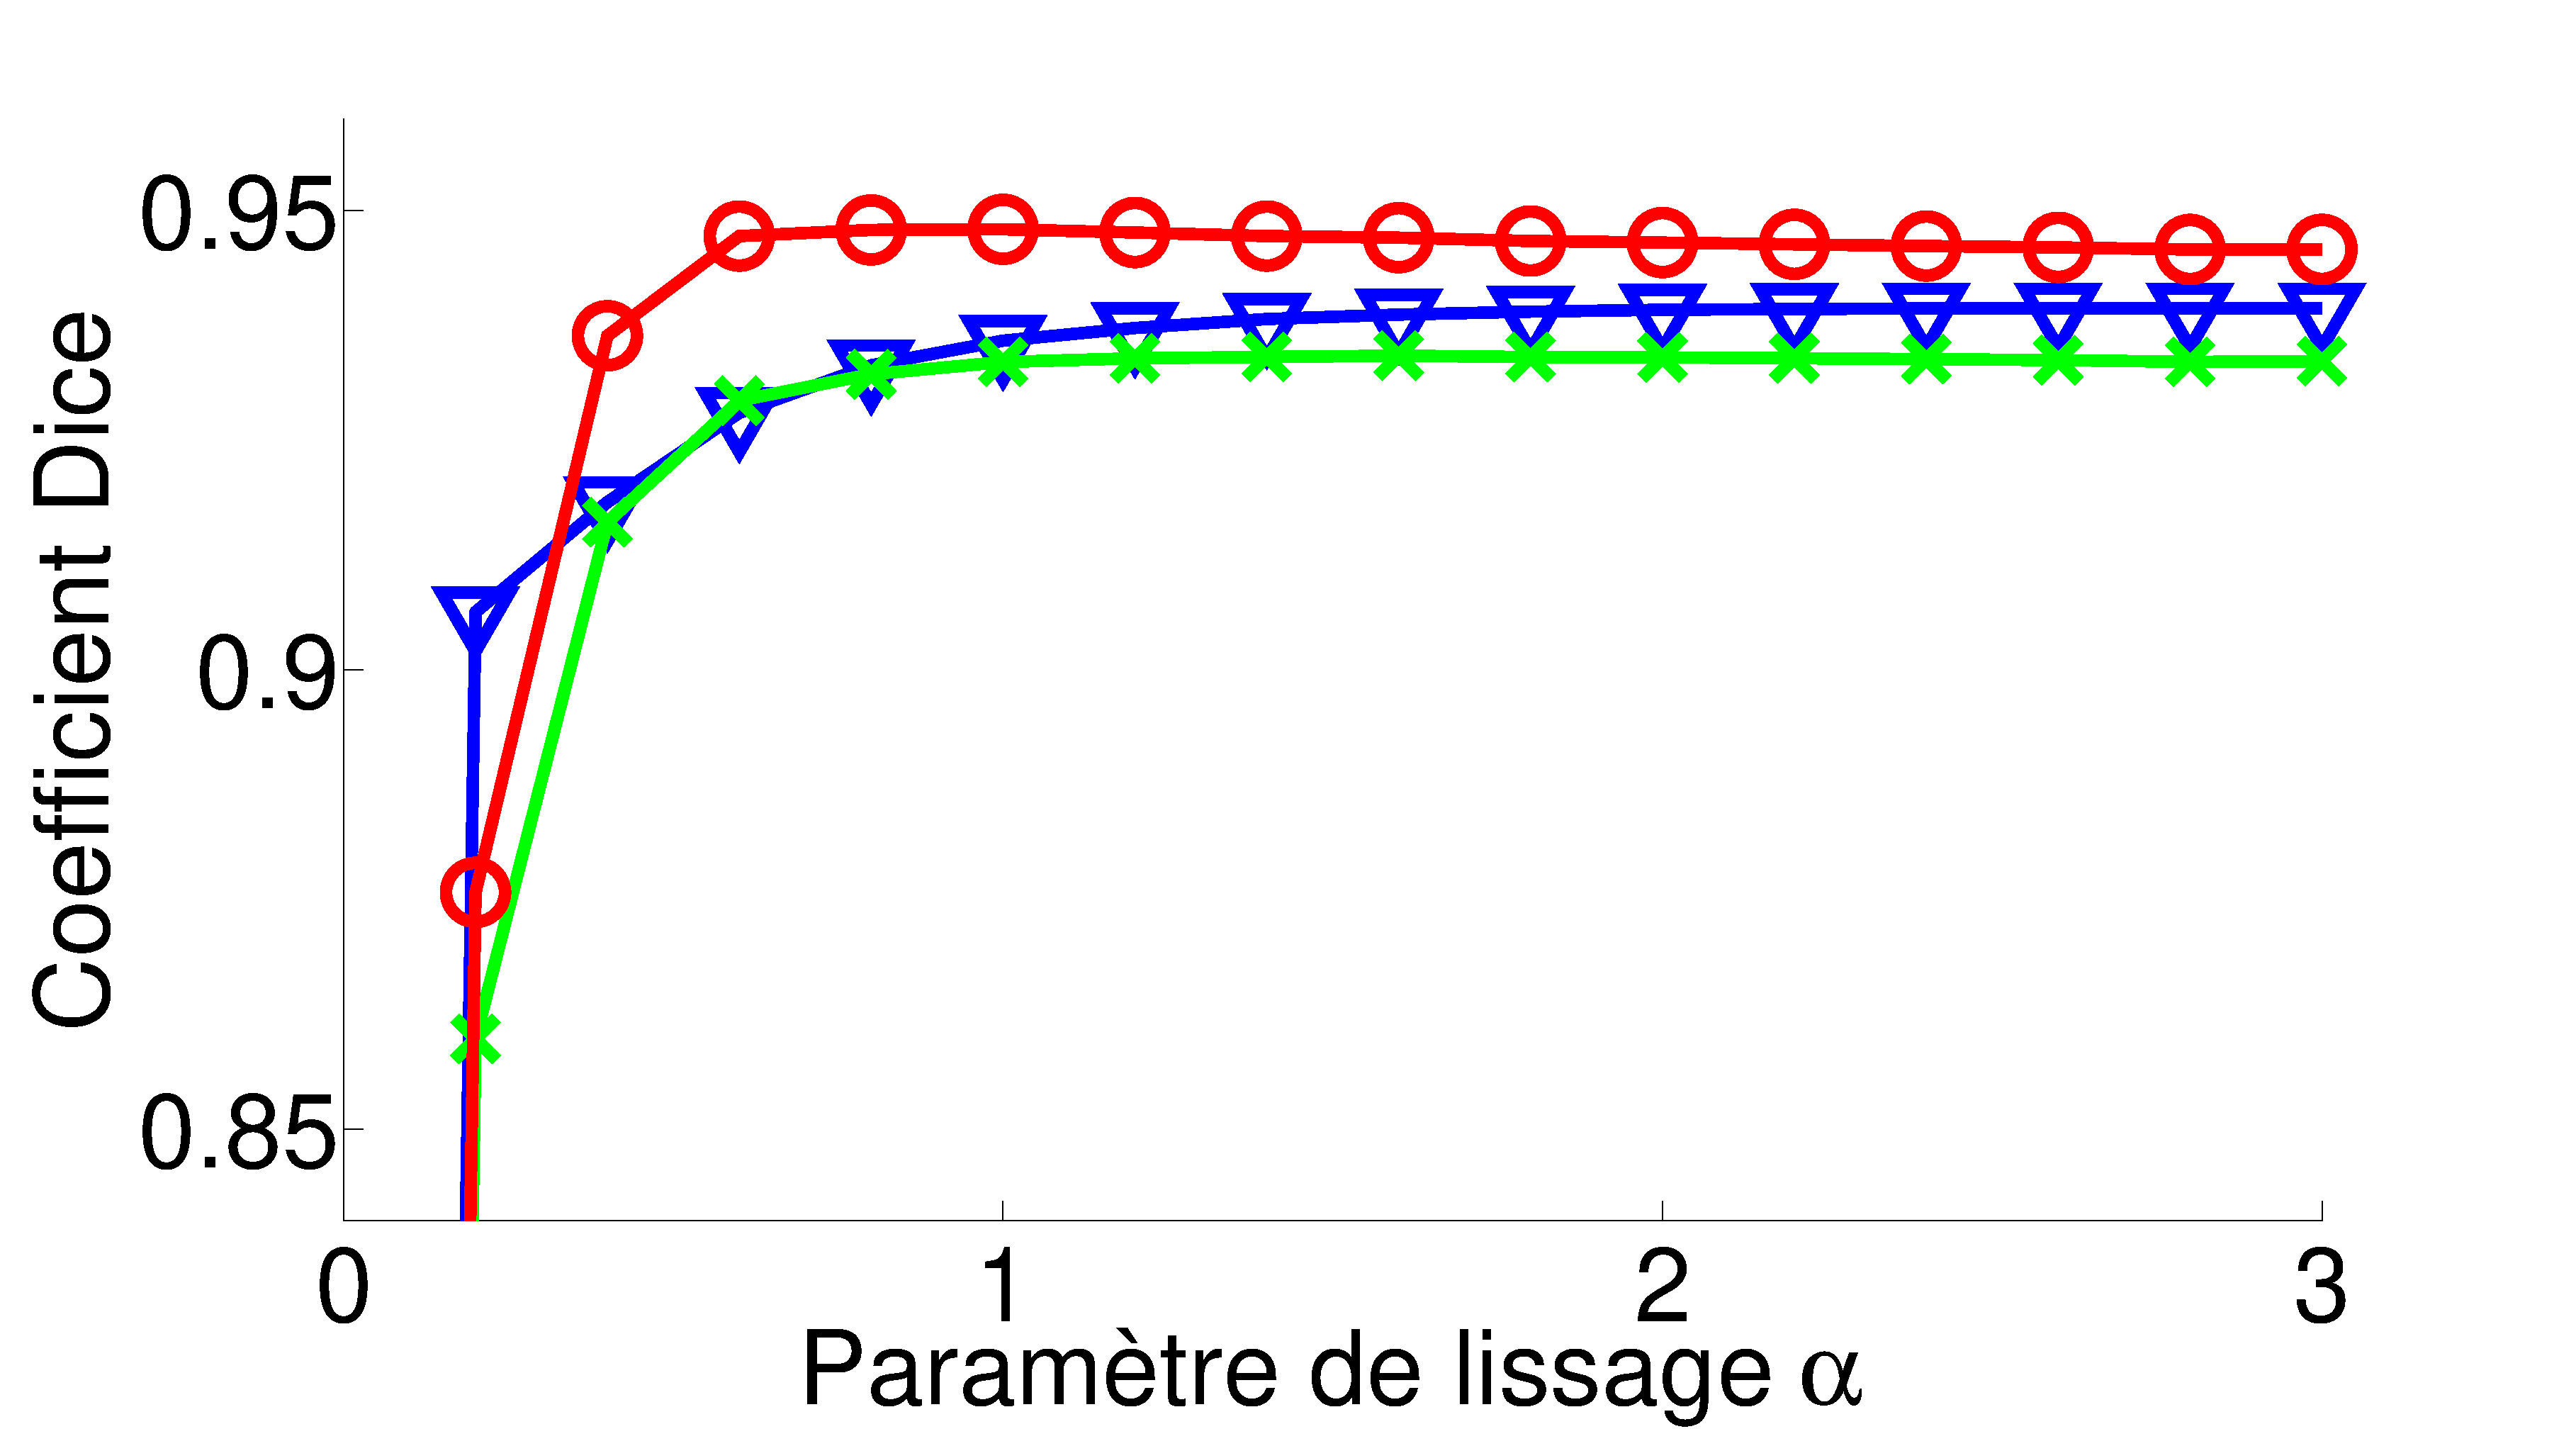
\includegraphics[height=38mm]{eps/chapitre3/nlreg_Dice_Smooth.eps}}
	\subfigure[]{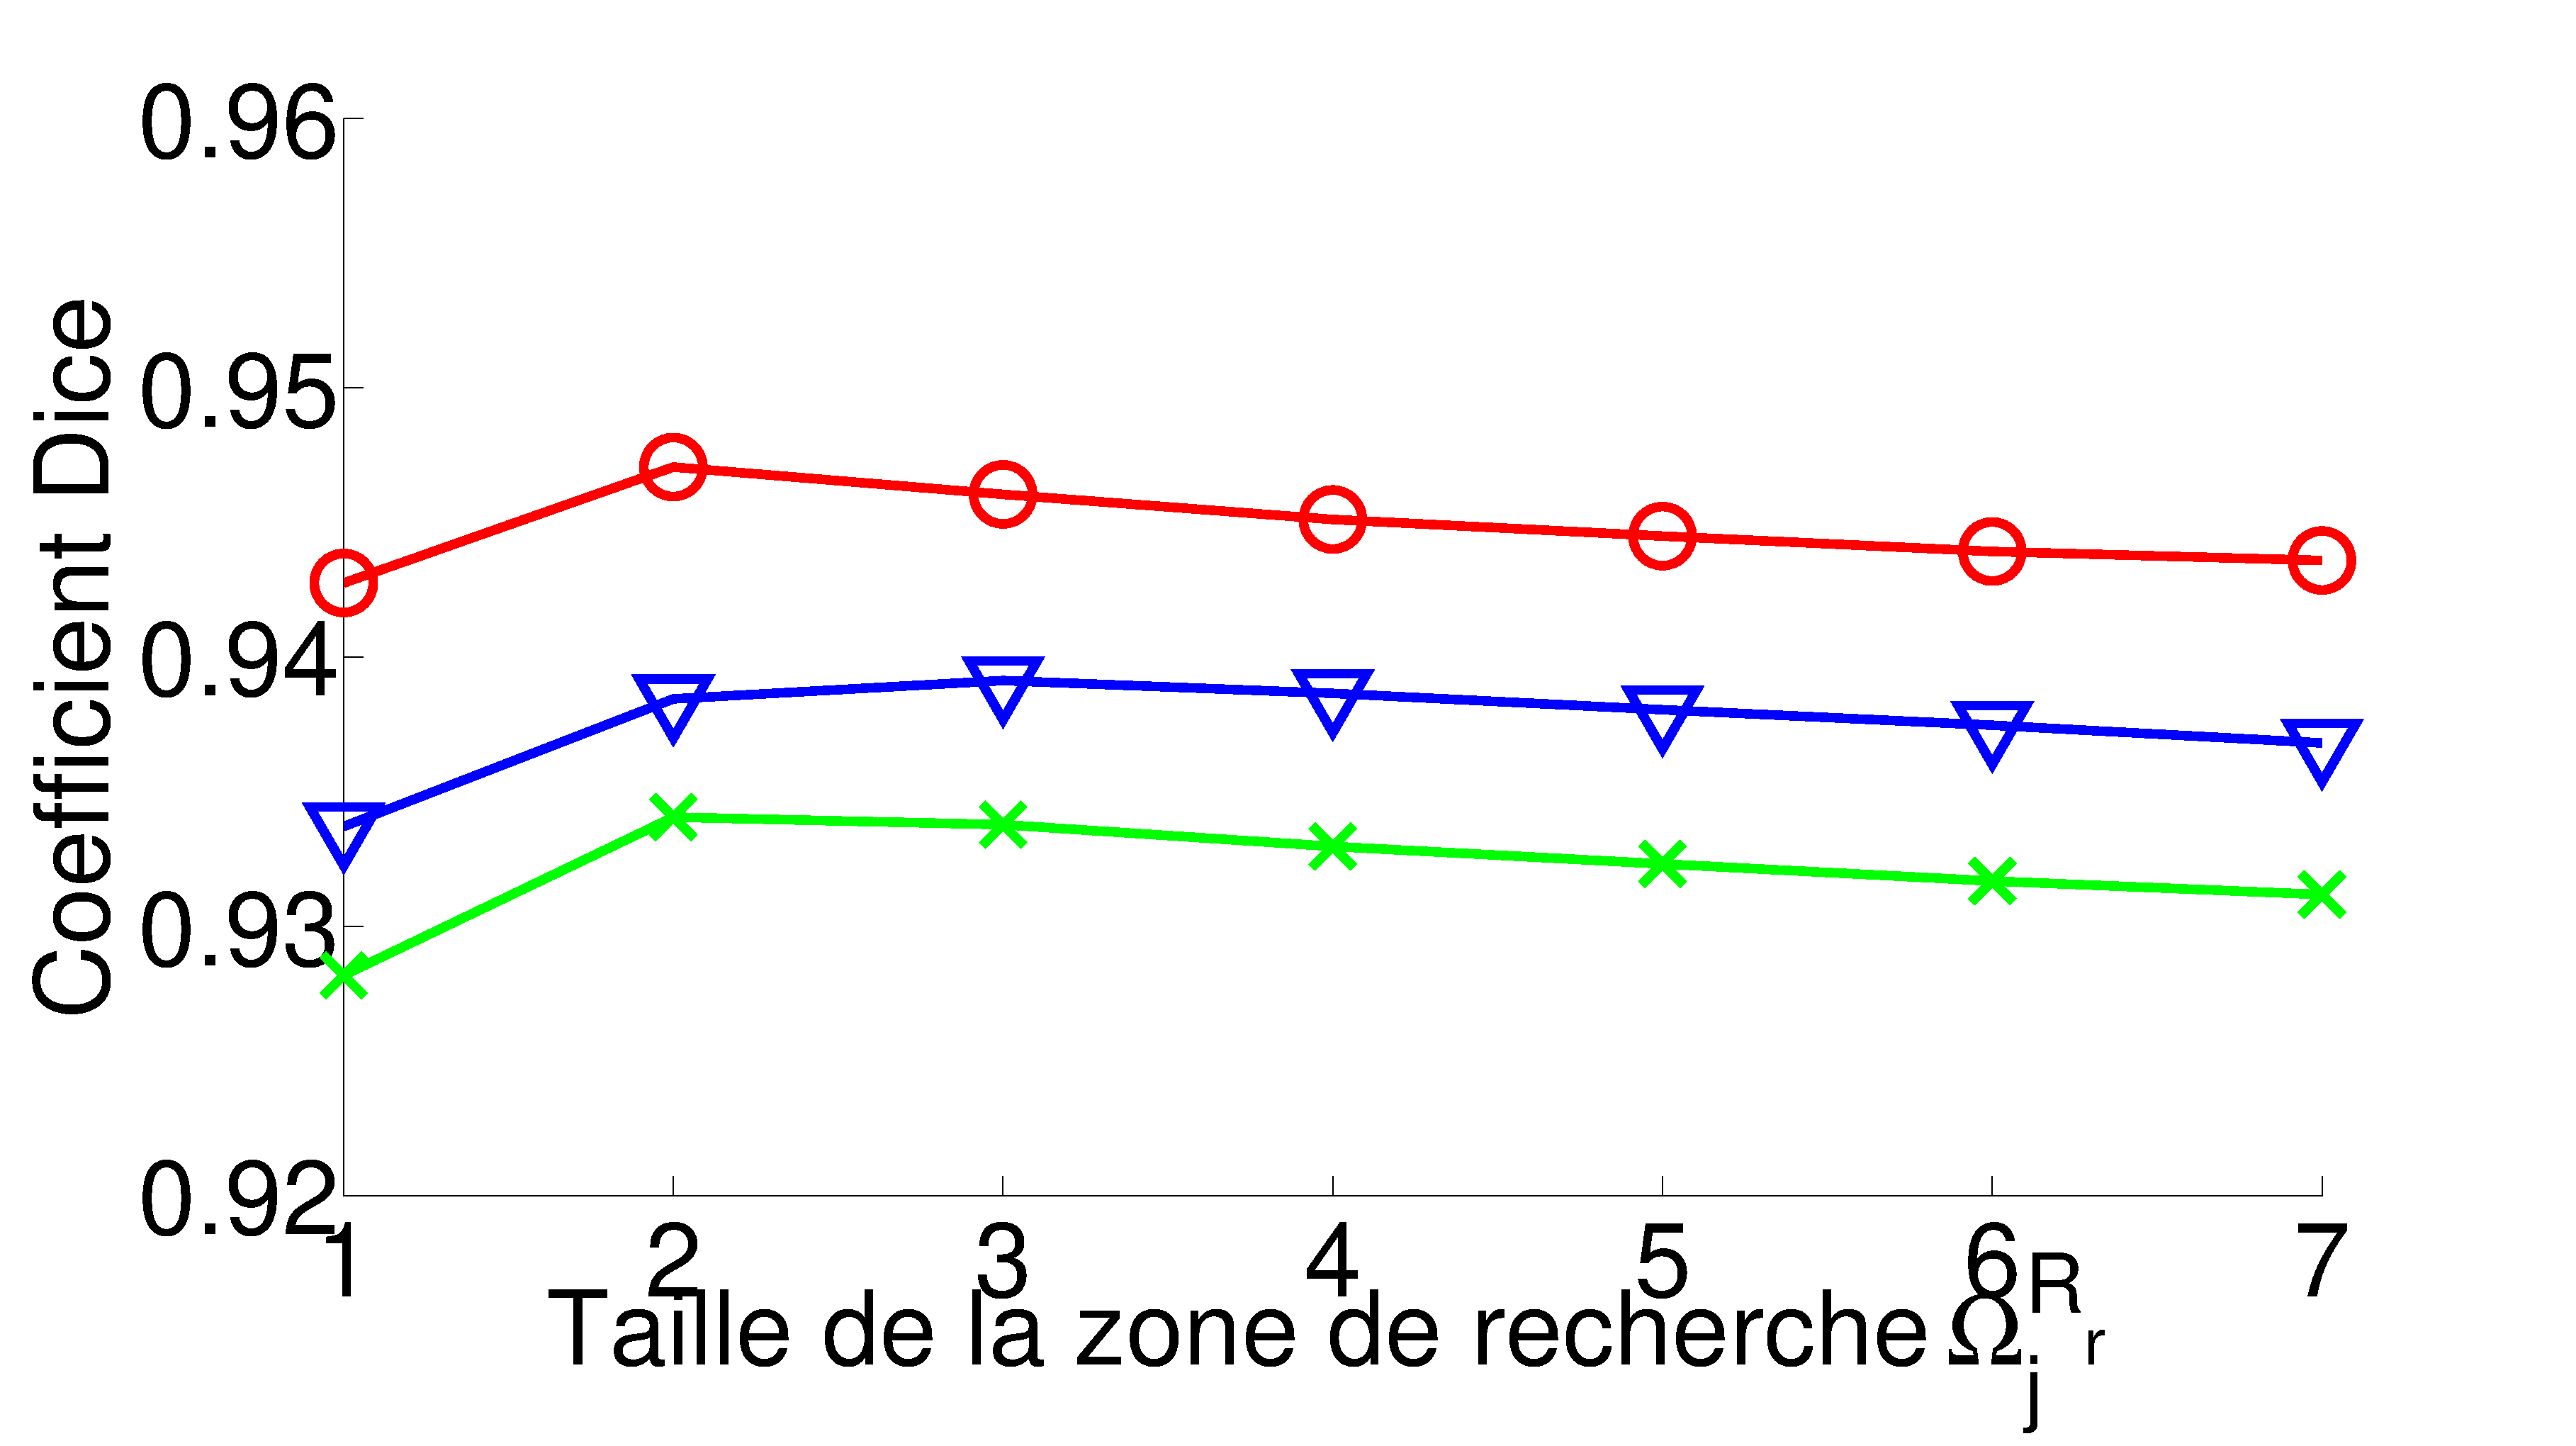
\includegraphics[height=38mm]{eps/chapitre3/nlreg_Dice_HWVS.eps}\label{FIG:PARAM:BRAINWEB:NOISE:HWVS}}
        \end{center}
        
        \caption{\emph{(a) Coefficient Dice en fonction du paramètre de lissage $\alpha$. (b) Coefficient Dice en fonction du rayon de la zone de recherche $\Omega^{R_{r}}_{j}$. LCR : $\bigtriangledown$, matière grise : $\times$, matière blanche : $\circ$.}}
        
        \label{FIG:PARAM:BRAINWEB:NOISE}

\end{figure}

Les paramètres testés sont la taille de la zone de recherche $\lvert \Omega^{R_{r}}_{j} \rvert$ ainsi que le paramètre de lissage $\alpha$.
La figure \ref{FIG:PARAM:BRAINWEB:NOISE} fournit une indication de l'influence de ces deux paramètres sur la segmentation.
Le paramètre de lissage $\alpha$ a une forte influence sur la segmentation s'il est situé entre $0$ et $1.5$, puis un phénomène de convergence est observé. 
Dans la suite du manuscrit, il sera fixé à $1.5$.
Concernant la taille de la zone de recherche, la figure~\ref{FIG:PARAM:BRAINWEB:NOISE:HWVS} montre un maximum du taux de recouvrement avec un rayon de $2$ voxels pour la matière blanche et la matière grise, et un maximum avec un rayon de $3$ voxels pour le LCR.
La taille de la zone de recherche $\Omega^{R_r}_{j}$ est donc fixée à $5\times5\times5$ pour la suite du manuscrit. 

\paragraph*{Comparaison par rapport à d'autres méthodologies}

La comparaison inclus une évaluation des méthodes FCM classique et RFCM \cite{Pham:CVIU:2001} en plus des méthodes markoviennes.
Elle est effectuée en simulant des segmentations avec un bruit ricien allant de $0$ à $9$~\%. 

La figure~\ref{FIG:VIEW:BRAINWEB:NOISE} présente une vue sur une coupe d'une image T1 et les segmentations correspondantes pour les algorithmes FCM classique, RFCM \cite{Pham:CVIU:2001} et NL-Reg.
L'apport de RFCM par rapport à l'algorithme FCM classique est visible par l'absence d'artefacts de segmentation dus au bruit (par exemple : voxels classés comme matière grise au milieu de la matière blanche).
Cependant, l'effet de lissage apporté par cette régularisation a pour effet de gommer les aspérités dans certaines parties de l'image. 
Par exemple, une comparaison visuelle avec la vérité terrain montre une sous-segmentation du LCR au sein des sillons.
Le terme de régularisation non-local permet de remédier à cela grâce à la pondération introduite par les poids non-locaux, ce qui est illustré par les figures~\ref{NLREG:ZOOM:TRUTH}, \ref{NLREG:ZOOM:RFCM} et \ref{NLREG:ZOOM:NLREG} montrant un zoom sur une zone particulière du cerveau.

De plus, la table~\ref{TAB:DICE:BRAINWEB:NOISE} montre une meilleure performance des algorithmes FCM que des algorithmes basés sur les champs et chaînes de Markov. 
La figure~\ref{FIG:DICE:BRAINWEB:NOISE}, comparant les coefficients Dice obtenus par les algorithmes en fonction du niveau de bruit, confirme cette observation.
Elle montre que le terme de régularisation non-local fournit une segmentation plus fiable à partir d'un niveau de bruit de $5$~\%.

\begin{table}[!htb]
\begin{center}
\begin{tabular}{|l | *{3}{c|}}
	\hline
	Méthodes & LCR & Matière grise & Matière blanche \\
	\hline
	FCM & 90.46 & 84.36 & 85.48\\
	RFCM & 92.09 & 91.12 & 92.91\\
% 	R-FCM with adaptive weights & 92.76 & 91.09 & 92.49\\
% 	NL-Reg without adaptive weights & 92.22 & 92.22 & 94.12\\
	NL-Reg & \fbox{93.63} & \fbox{93.35} & \fbox{94.77}\\
	SPM5 & 54.2 & 85.1 & 87 \\
	EMS & 89.6 & 86.9 & 90.9\\
	HMC & 68 & 86.5 & 87.1\\
	\hline 
\end{tabular}
% \vspace{2mm}
\caption{\emph{Application de différentes segmentations à une image pondérée en T1 avec un bruit ricien de $9$~\%. Comparaison des différents coefficient Dice pour le LCR, la matière grise et la matière blanche.\label{TAB:DICE:BRAINWEB:NOISE}}}
\end{center}
\end{table}

\begin{figure}[!thbp]
\begin{center}
\subfigure[]{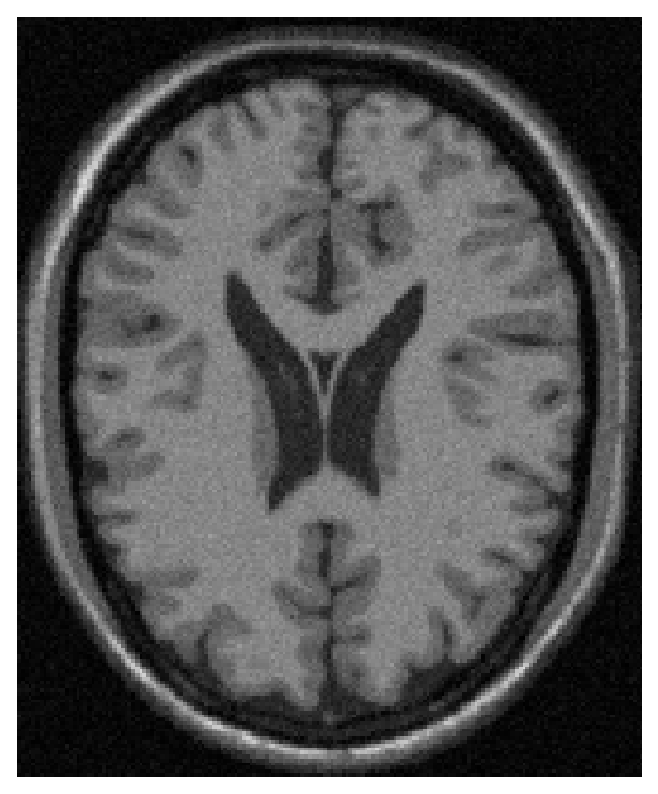
\includegraphics[height=45mm]{eps/chapitre3/Brainweb_Noise_T1.eps}}  
\subfigure[]{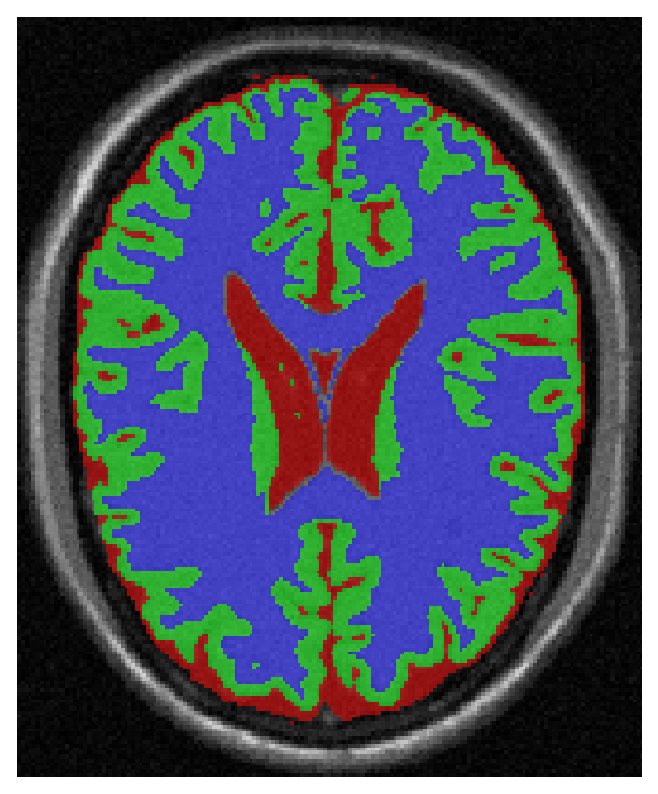
\includegraphics[height=45mm]{eps/chapitre3/Brainweb_Noise_truth.eps}}\\
\subfigure[]{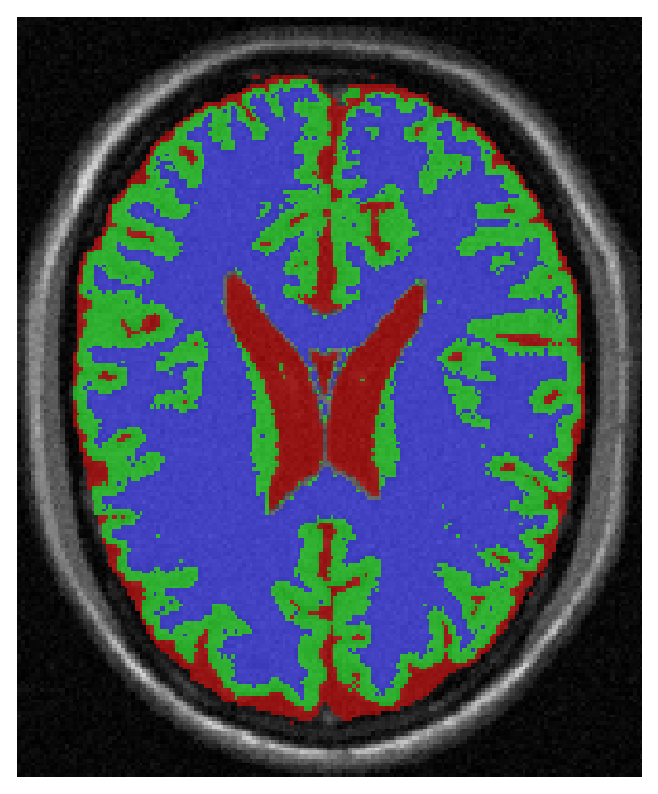
\includegraphics[height=45mm]{eps/chapitre3/Brainweb_Noise_classicfcm.eps}}  
\subfigure[]{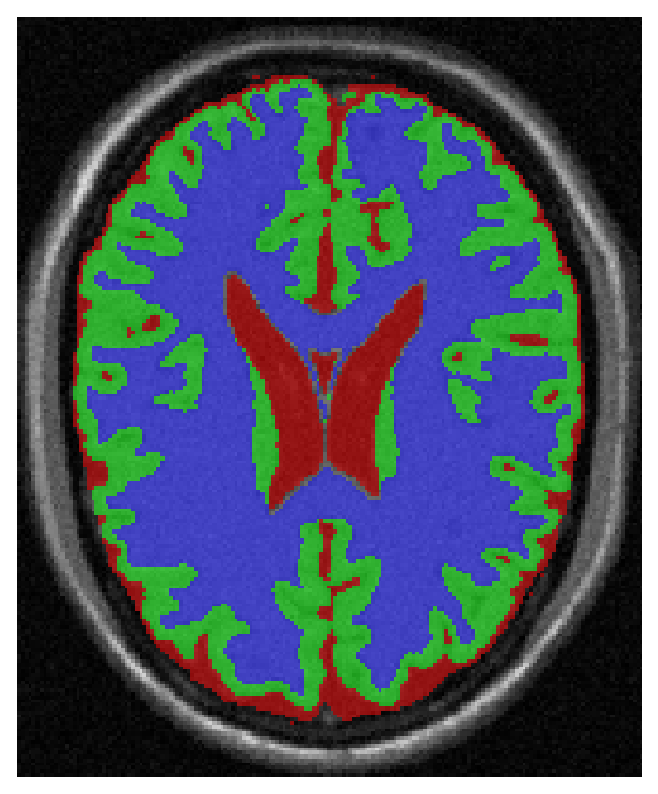
\includegraphics[height=45mm]{eps/chapitre3/Brainweb_Noise_rfcm.eps}}  
\subfigure[]{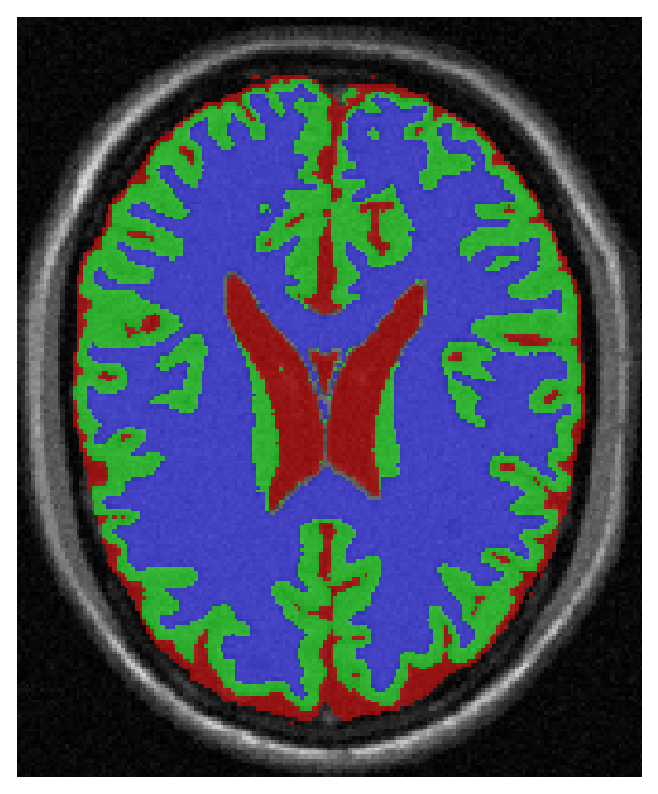
\includegraphics[height=45mm]{eps/chapitre3/Brainweb_Noise_nlregfcm.eps}}\\
\subfigure[]{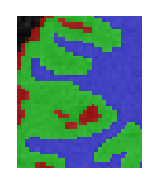
\includegraphics[height=45mm]{eps/chapitre3/Brainweb_Noise_truth_zoom.eps}\label{NLREG:ZOOM:TRUTH}}  
\subfigure[]{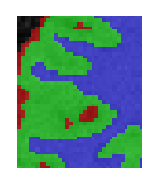
\includegraphics[height=45mm]{eps/chapitre3/Brainweb_Noise_rfcm_zoom.eps}\label{NLREG:ZOOM:RFCM}}  
\subfigure[]{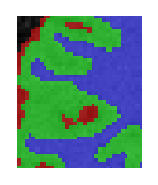
\includegraphics[height=45mm]{eps/chapitre3/Brainweb_Noise_nlregfcm_zoom.eps}\label{NLREG:ZOOM:NLREG}}\\
\caption{\emph{(a) Coupe axiale d'une image pondérée T1 avec un bruit ricien à $5$~\%. (b) Vérité terrain. (c) Segmentation par FCM classique. (d) Segmentation par RFCM~\cite{Pham:CVIU:2001}. (e) Segmentation par NL-Reg. (f) Zoom sur la vérité terrain. (g) Zoom sur la segmentation par RFCM. (h) Zoom sur la segmentation par NL-Reg.}\label{FIG:VIEW:BRAINWEB:NOISE}}
\end{center}
\end{figure}

\begin{figure}[!thbp]
\begin{center}
\subfigure[]{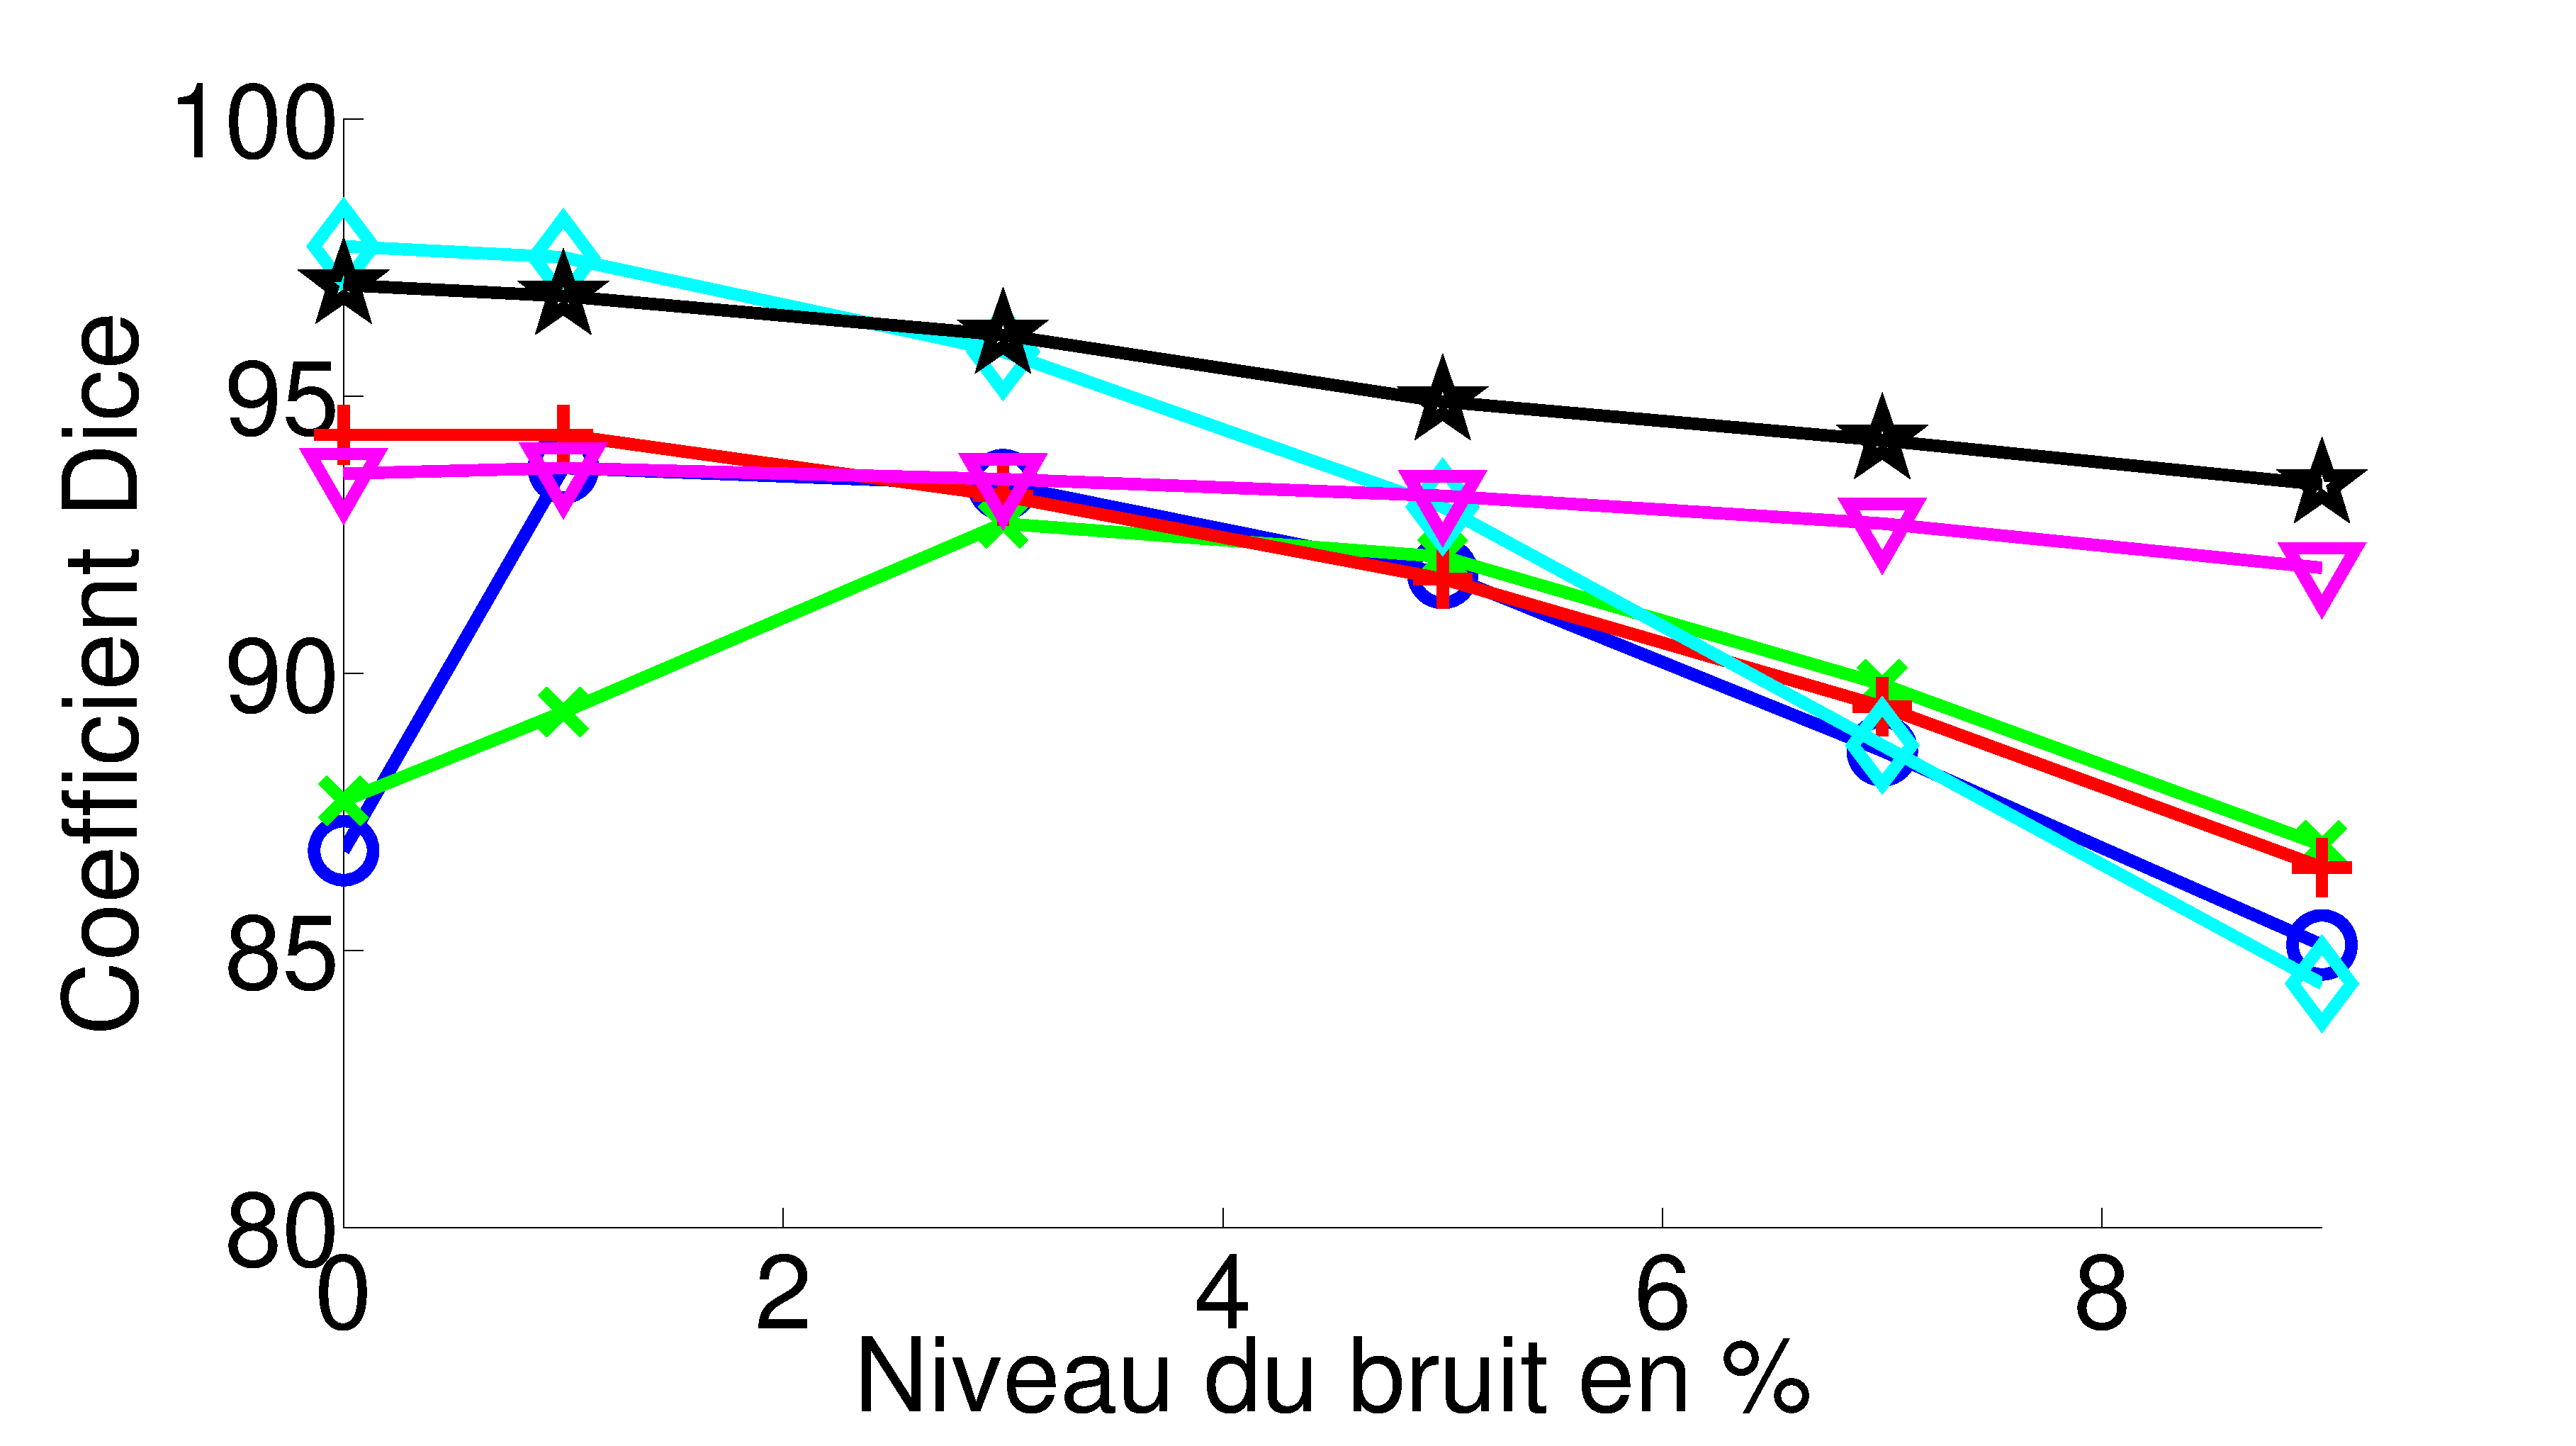
\includegraphics[height=38mm]{eps/chapitre3/GM_Noise_Dice_Brainweb.eps}}  
\subfigure[]{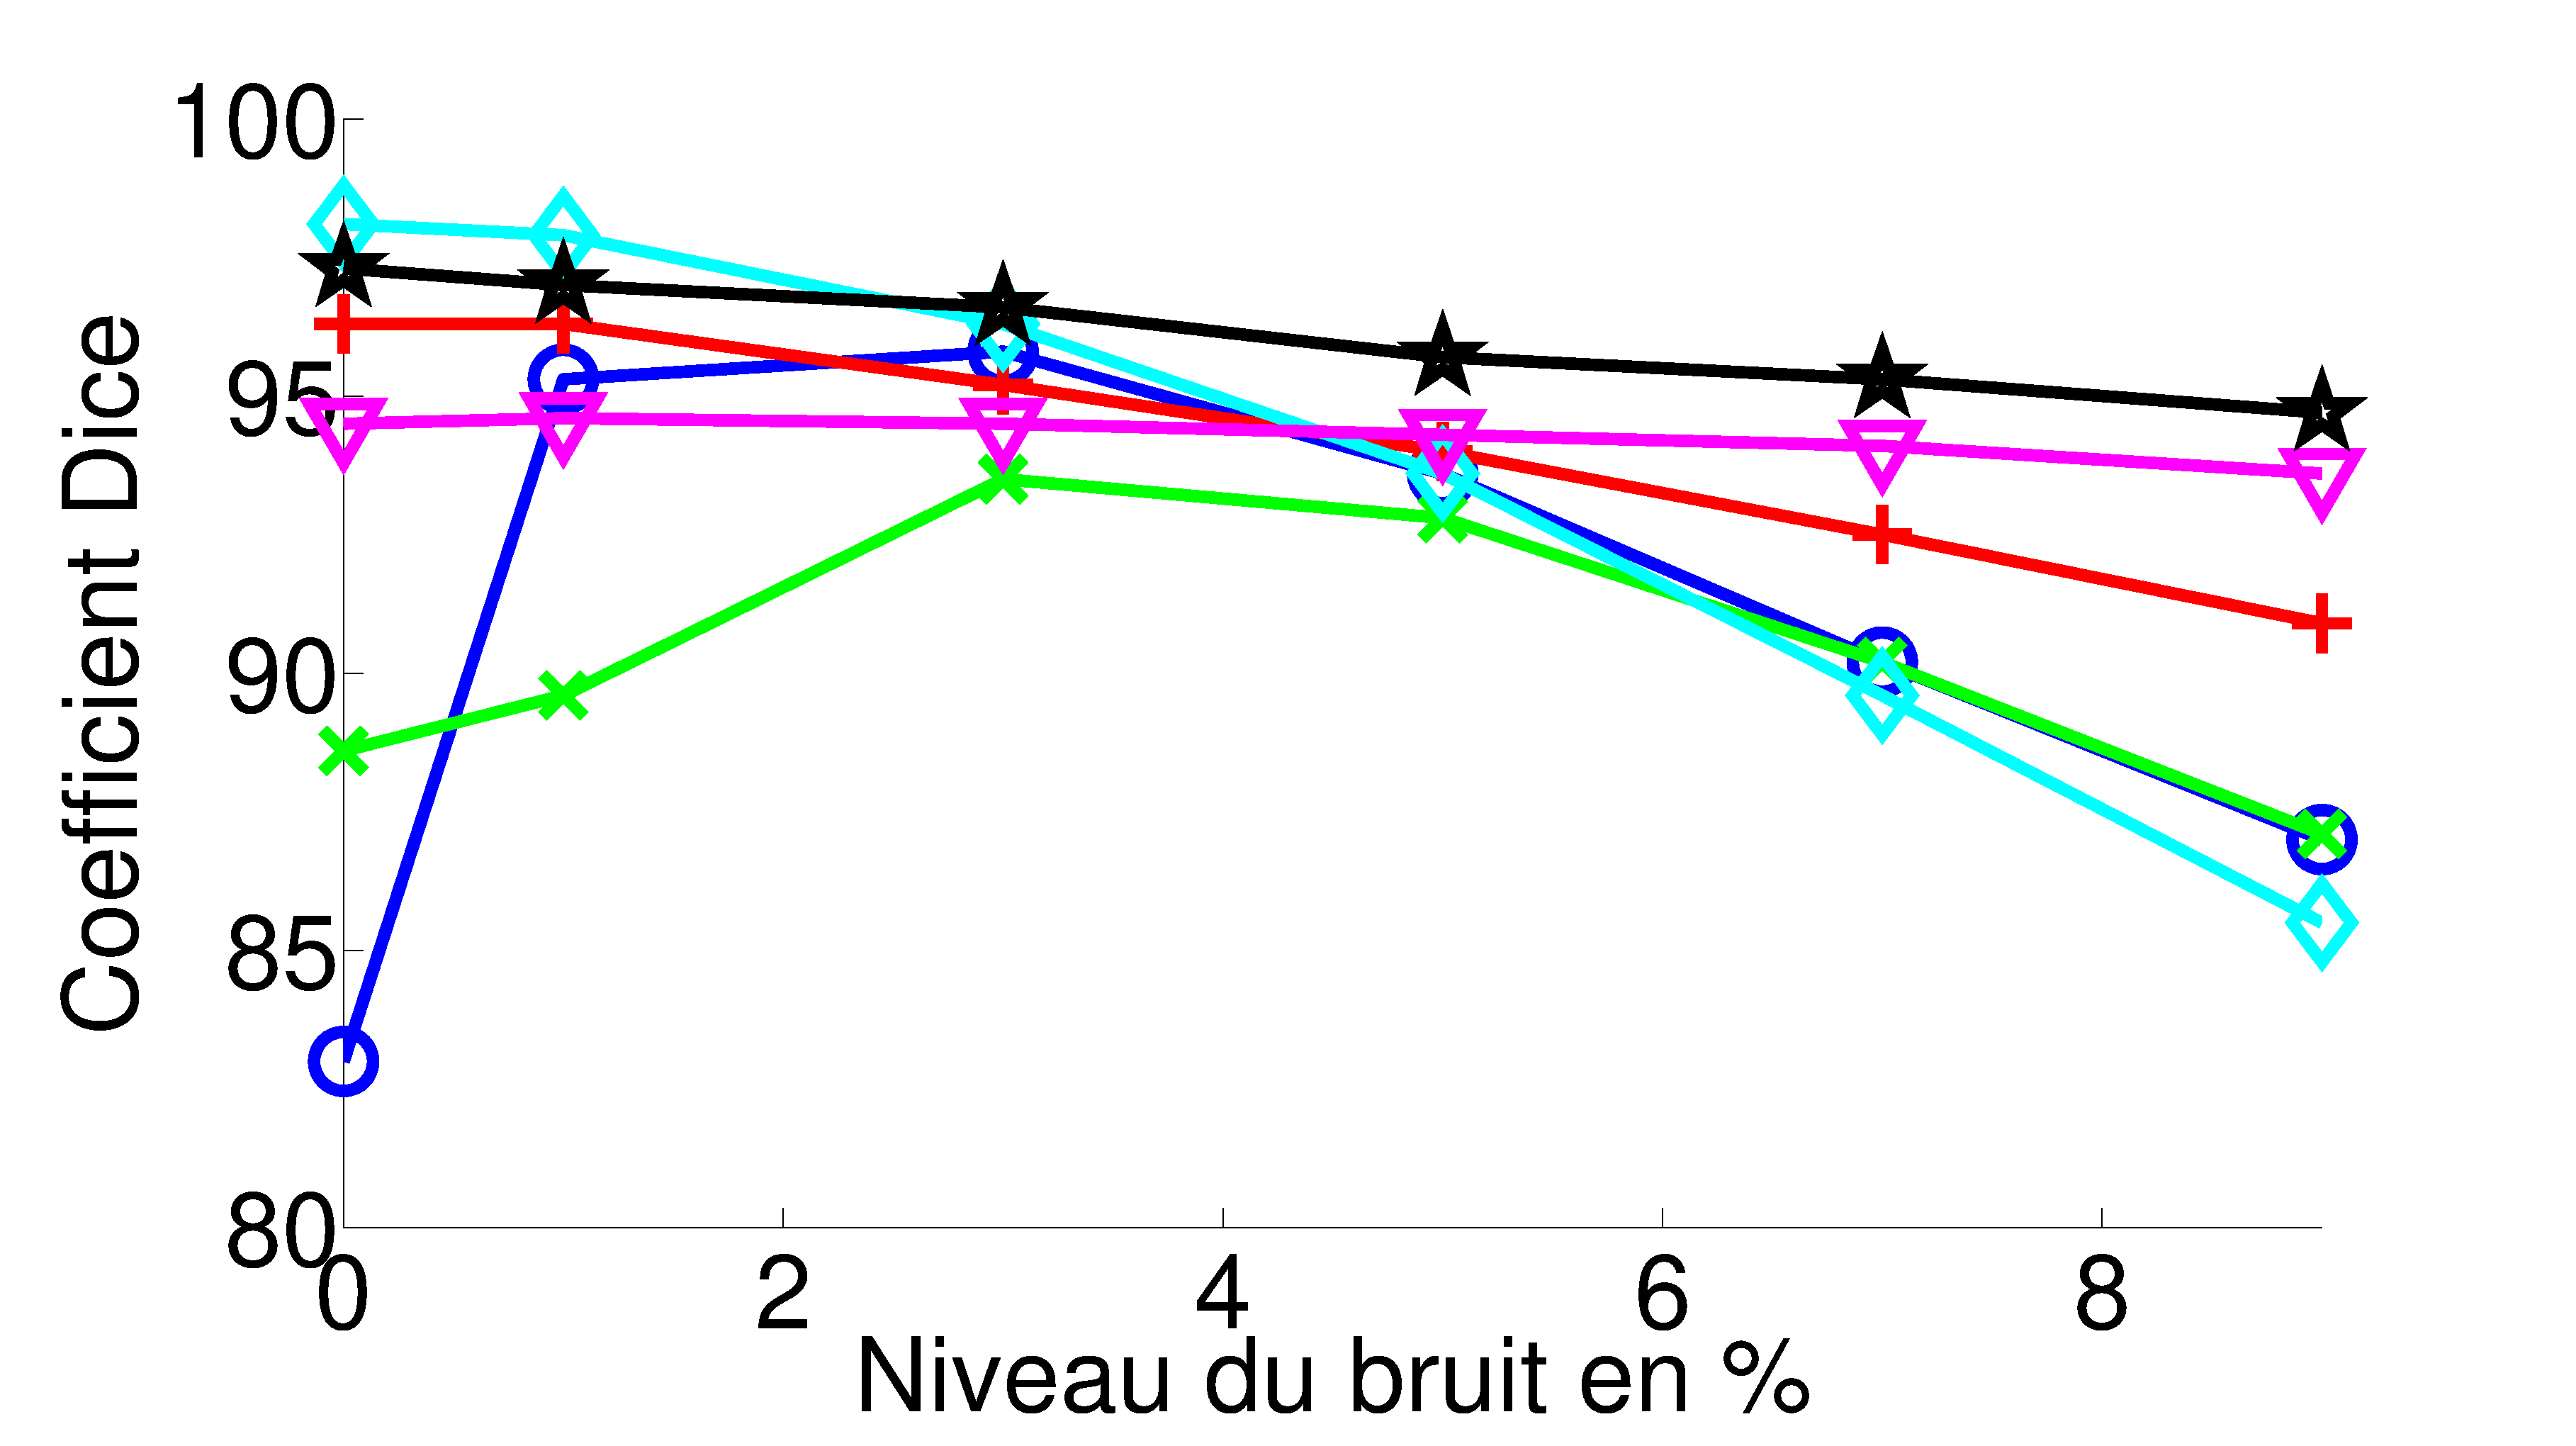
\includegraphics[height=38mm]{eps/chapitre3/WM_Noise_Dice_Brainweb.eps}}  
\caption{\emph{Evolution du coefficient Dice en fonction du bruit pour différentes méthodologies. (a) Matière grise. (b) Matière blanche. Légende : SPM5 : $\circ$, EMS : $\times$, HMC : $+$, FCM : $\diamond$, RFCM : $\bigtriangledown$, NL-Reg : $\star$.}\label{FIG:DICE:BRAINWEB:NOISE}}
\end{center}
\end{figure}

\subsubsection{Association des termes d'attache aux données et de régularisation non-locaux}
\label{sec:brainweb:nlAll}

% L'association des termes non-locaux devrait permettre de segmenter des images corrompues par un biais en intensité et par un bruit ricien. 
% Au cours de ces expériences, le biais en intensité est de l'ordre de 20\% et le bruit est de type Ricien allant de 1\% à 9\%.
Dans cette section, l'association des termes d'attache aux données et de régularisation non-locaux est évaluée.
Les images utilisées présentent un biais en intensité de $20$~\% et un bruit de type ricien d'un niveau allant de $1$~\% à $9$~\%.
Les paramètres considérés sont les suivants : 
\begin{itemize}
\item la taille des sous-volumes destinés à évaluer le modèle de la distribution d'intensité est fixée à $M_j = 17\times17\times17$, 
\item la taille de la zone de recherche destinée au calcul des poids non-locaux du terme d'attache aux données est fixée à $\Omega^{R_{d}}_{j} = 17\times17\times17$, 
\item la taille de la zone de recherche destinée au calcul des poids non-locaux du terme de régularisation est fixée à $\Omega^{R_{r}}_{j} = 5\times5\times5$,
\item le paramètre de lissage pour le calcul des poids non-locaux est fixé à $\alpha = 1.5$.
\end{itemize}

Les résultats sont fournis par la figure~\ref{FIG:VIEW:BRAINWEB:ALL} et la table~\ref{TAB:DICE:BRAINWEB:ALL}.
Comme attendu, l'utilisation du terme d'attache aux données non-local permet d'améliorer largement les performances par comparaison avec l'algorithme FCM original.
De plus, l'ajout du terme de régularisation non-local permet de combiner les avantages des deux termes et de fournir une segmentation fiable malgré la présence d'un biais en intensité et de bruit.
% De plus, l'utilisation simultanée des termes non-locaux amène une amélioration conjointe des résultats et permet d'obtenir de meilleurs résultats finaux.

\begin{figure}[!thbp]

        \begin{center}
	\subfigure[]{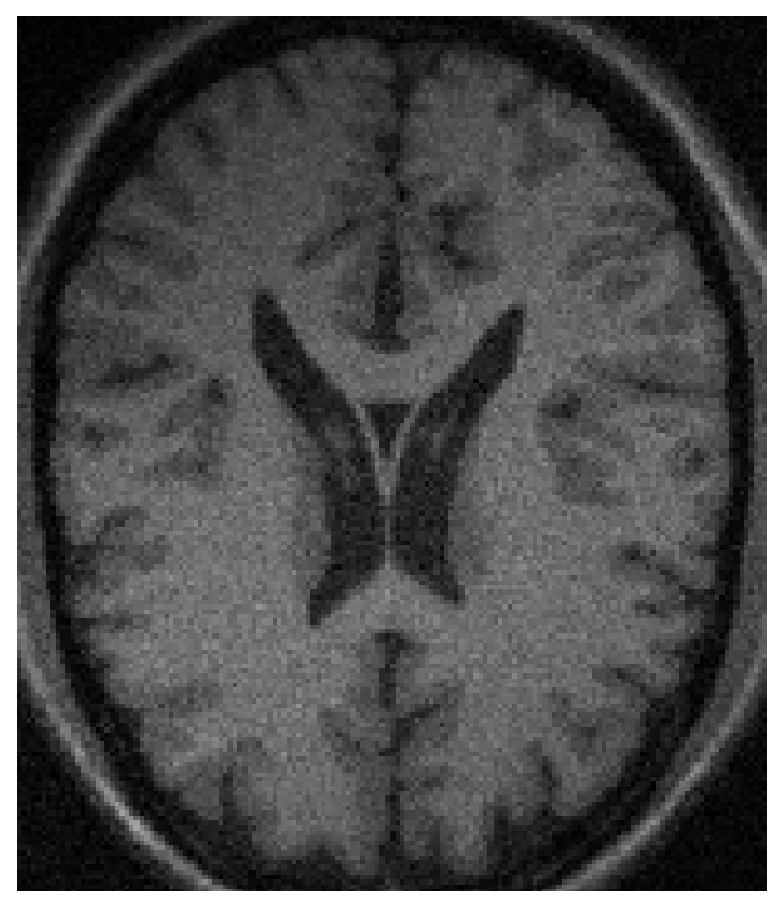
\includegraphics[height=41mm]{eps/chapitre3/Brainweb_All_T1.eps}}
	\subfigure[]{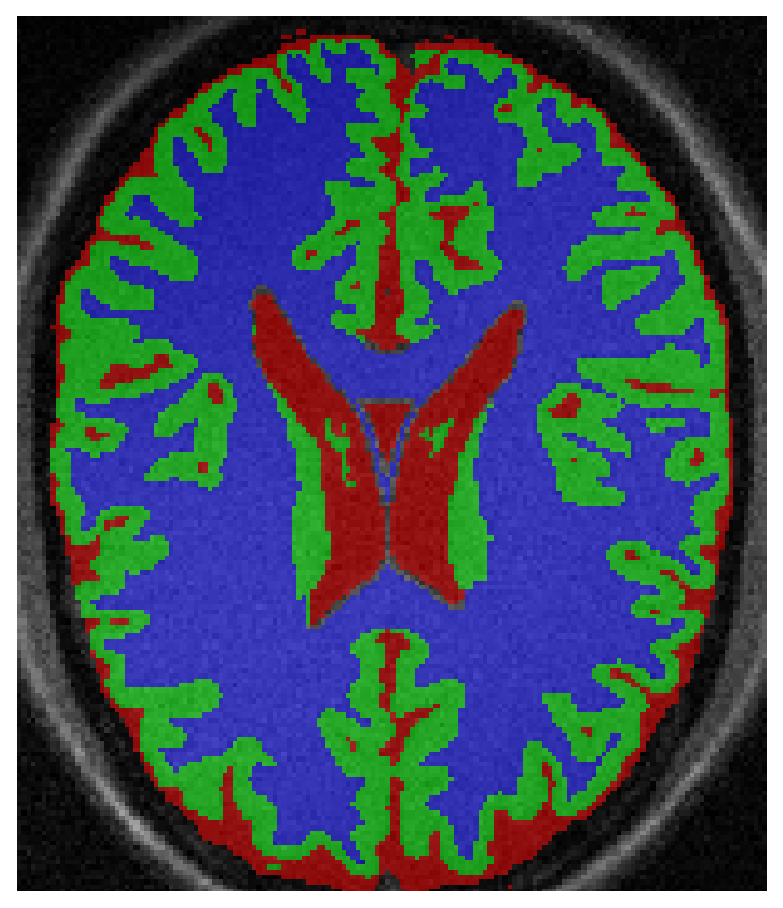
\includegraphics[height=41mm]{eps/chapitre3/Brainweb_All_Truth.eps}}\\
	\subfigure[]{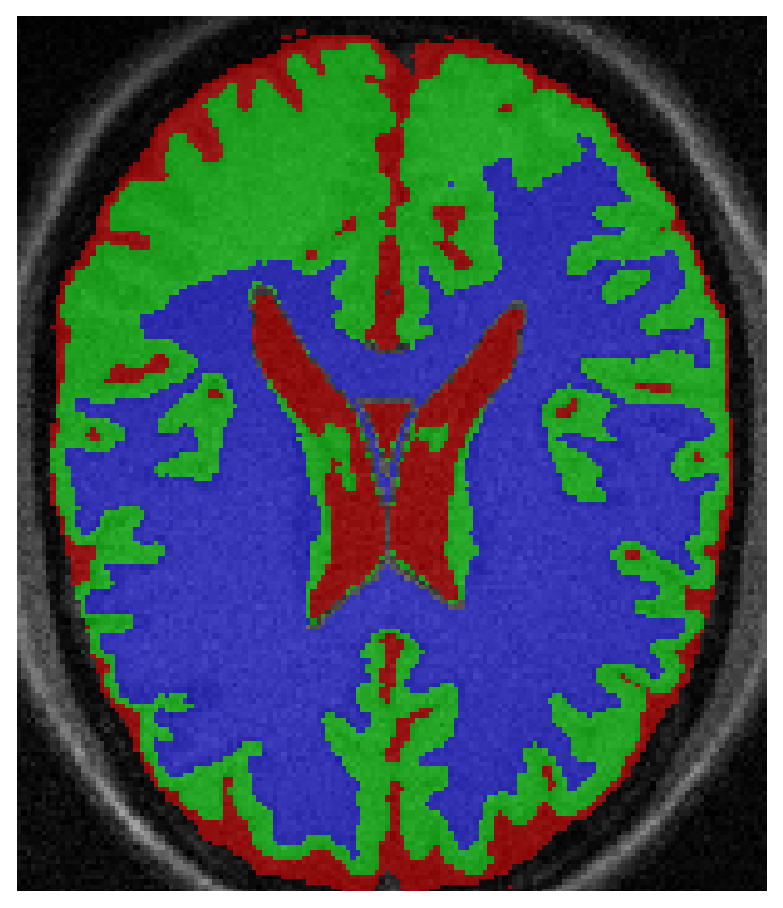
\includegraphics[height=41mm]{eps/chapitre3/Brainweb_All_NLReg.eps}}
	\subfigure[]{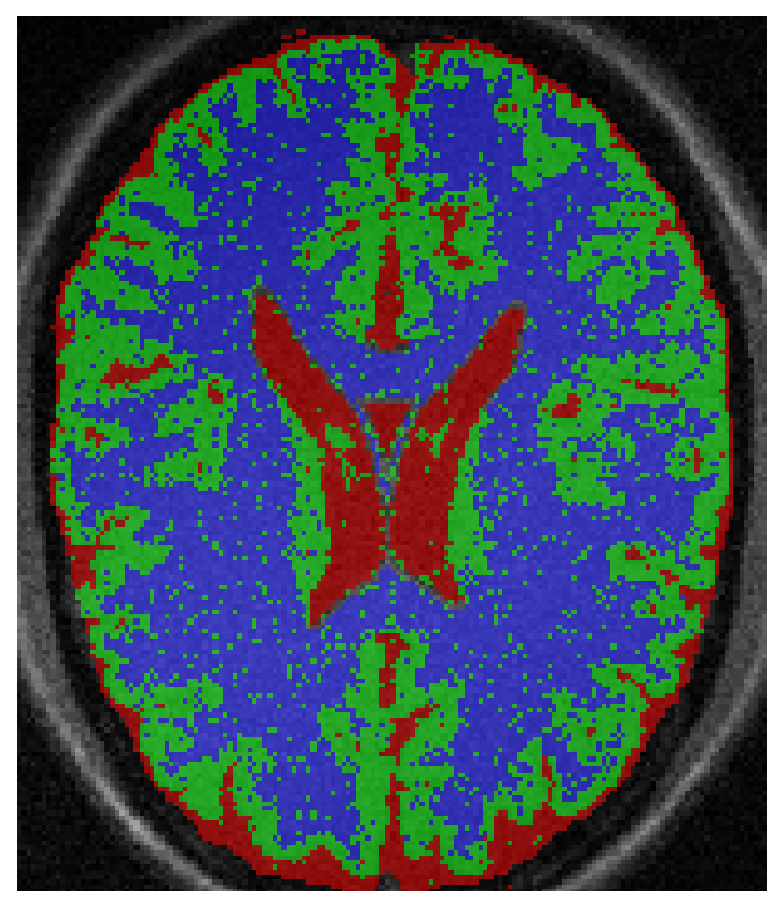
\includegraphics[height=41mm]{eps/chapitre3/Brainweb_All_NLFCM.eps}}
	\subfigure[]{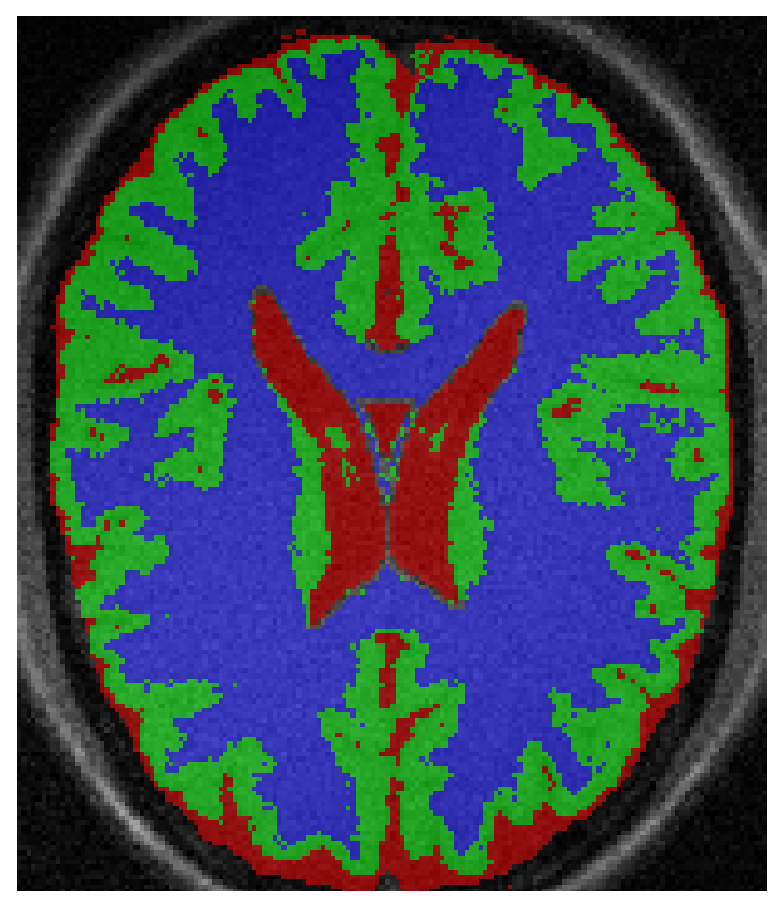
\includegraphics[height=41mm]{eps/chapitre3/Brainweb_All_NLRFCM.eps}}
        \end{center}

        \caption{\emph{Résultats de la segmentation d'une image T1 présentant une inhomogénéité en intensité et un bruit ricien de $9$~\%. (a) Coupe d'une image T1. (b) Vérité terrain. (c) Segmentation par NL-Reg. (d) Segmentation par NL-FCM. (e) Segmentation par NL-R-FCM.}}

        \label{FIG:VIEW:BRAINWEB:ALL}

\end{figure}

\begin{table}[!htb]
\begin{center}
\begin{tabular}{|l | *{2}{c|}}
	\hline
	Méthodes & Matière grise & Matière blanche \\
	\hline
	SPM5 & 85.1 & 87 \\ 
	EMS & 86.9 & 87.1 \\
	HMC & \fbox{86.5} & \fbox{90.9}  \\
	\hline
	FCM \cite{Pham:TMI:1999} &  62.09 & 69.98\\
	NL-Reg  & 64.25 & 72.16\\
	NL-FCM & 82.0 & 84.7\\
	NL-R-FCM & \fbox{86.5} & 89.2\\
	\hline 
\end{tabular}
\vspace{2mm}
\caption{Application de différentes segmentation sur une image T1 issue de BrainWeb avec un bruit Ricien à $9$~\% et un biais en intensité de $20$~\%. Comparaison des différents coefficient Dice pour la matière grise et la matière blanche (Coefficients Dice pour SPM5, EMS et HMC issus de \cite{Bricq:MIA:2008}).\label{TAB:DICE:BRAINWEB:ALL}}
\end{center}
\end{table}

\begin{figure}[!thbp]

        \begin{center}
	\subfigure[]{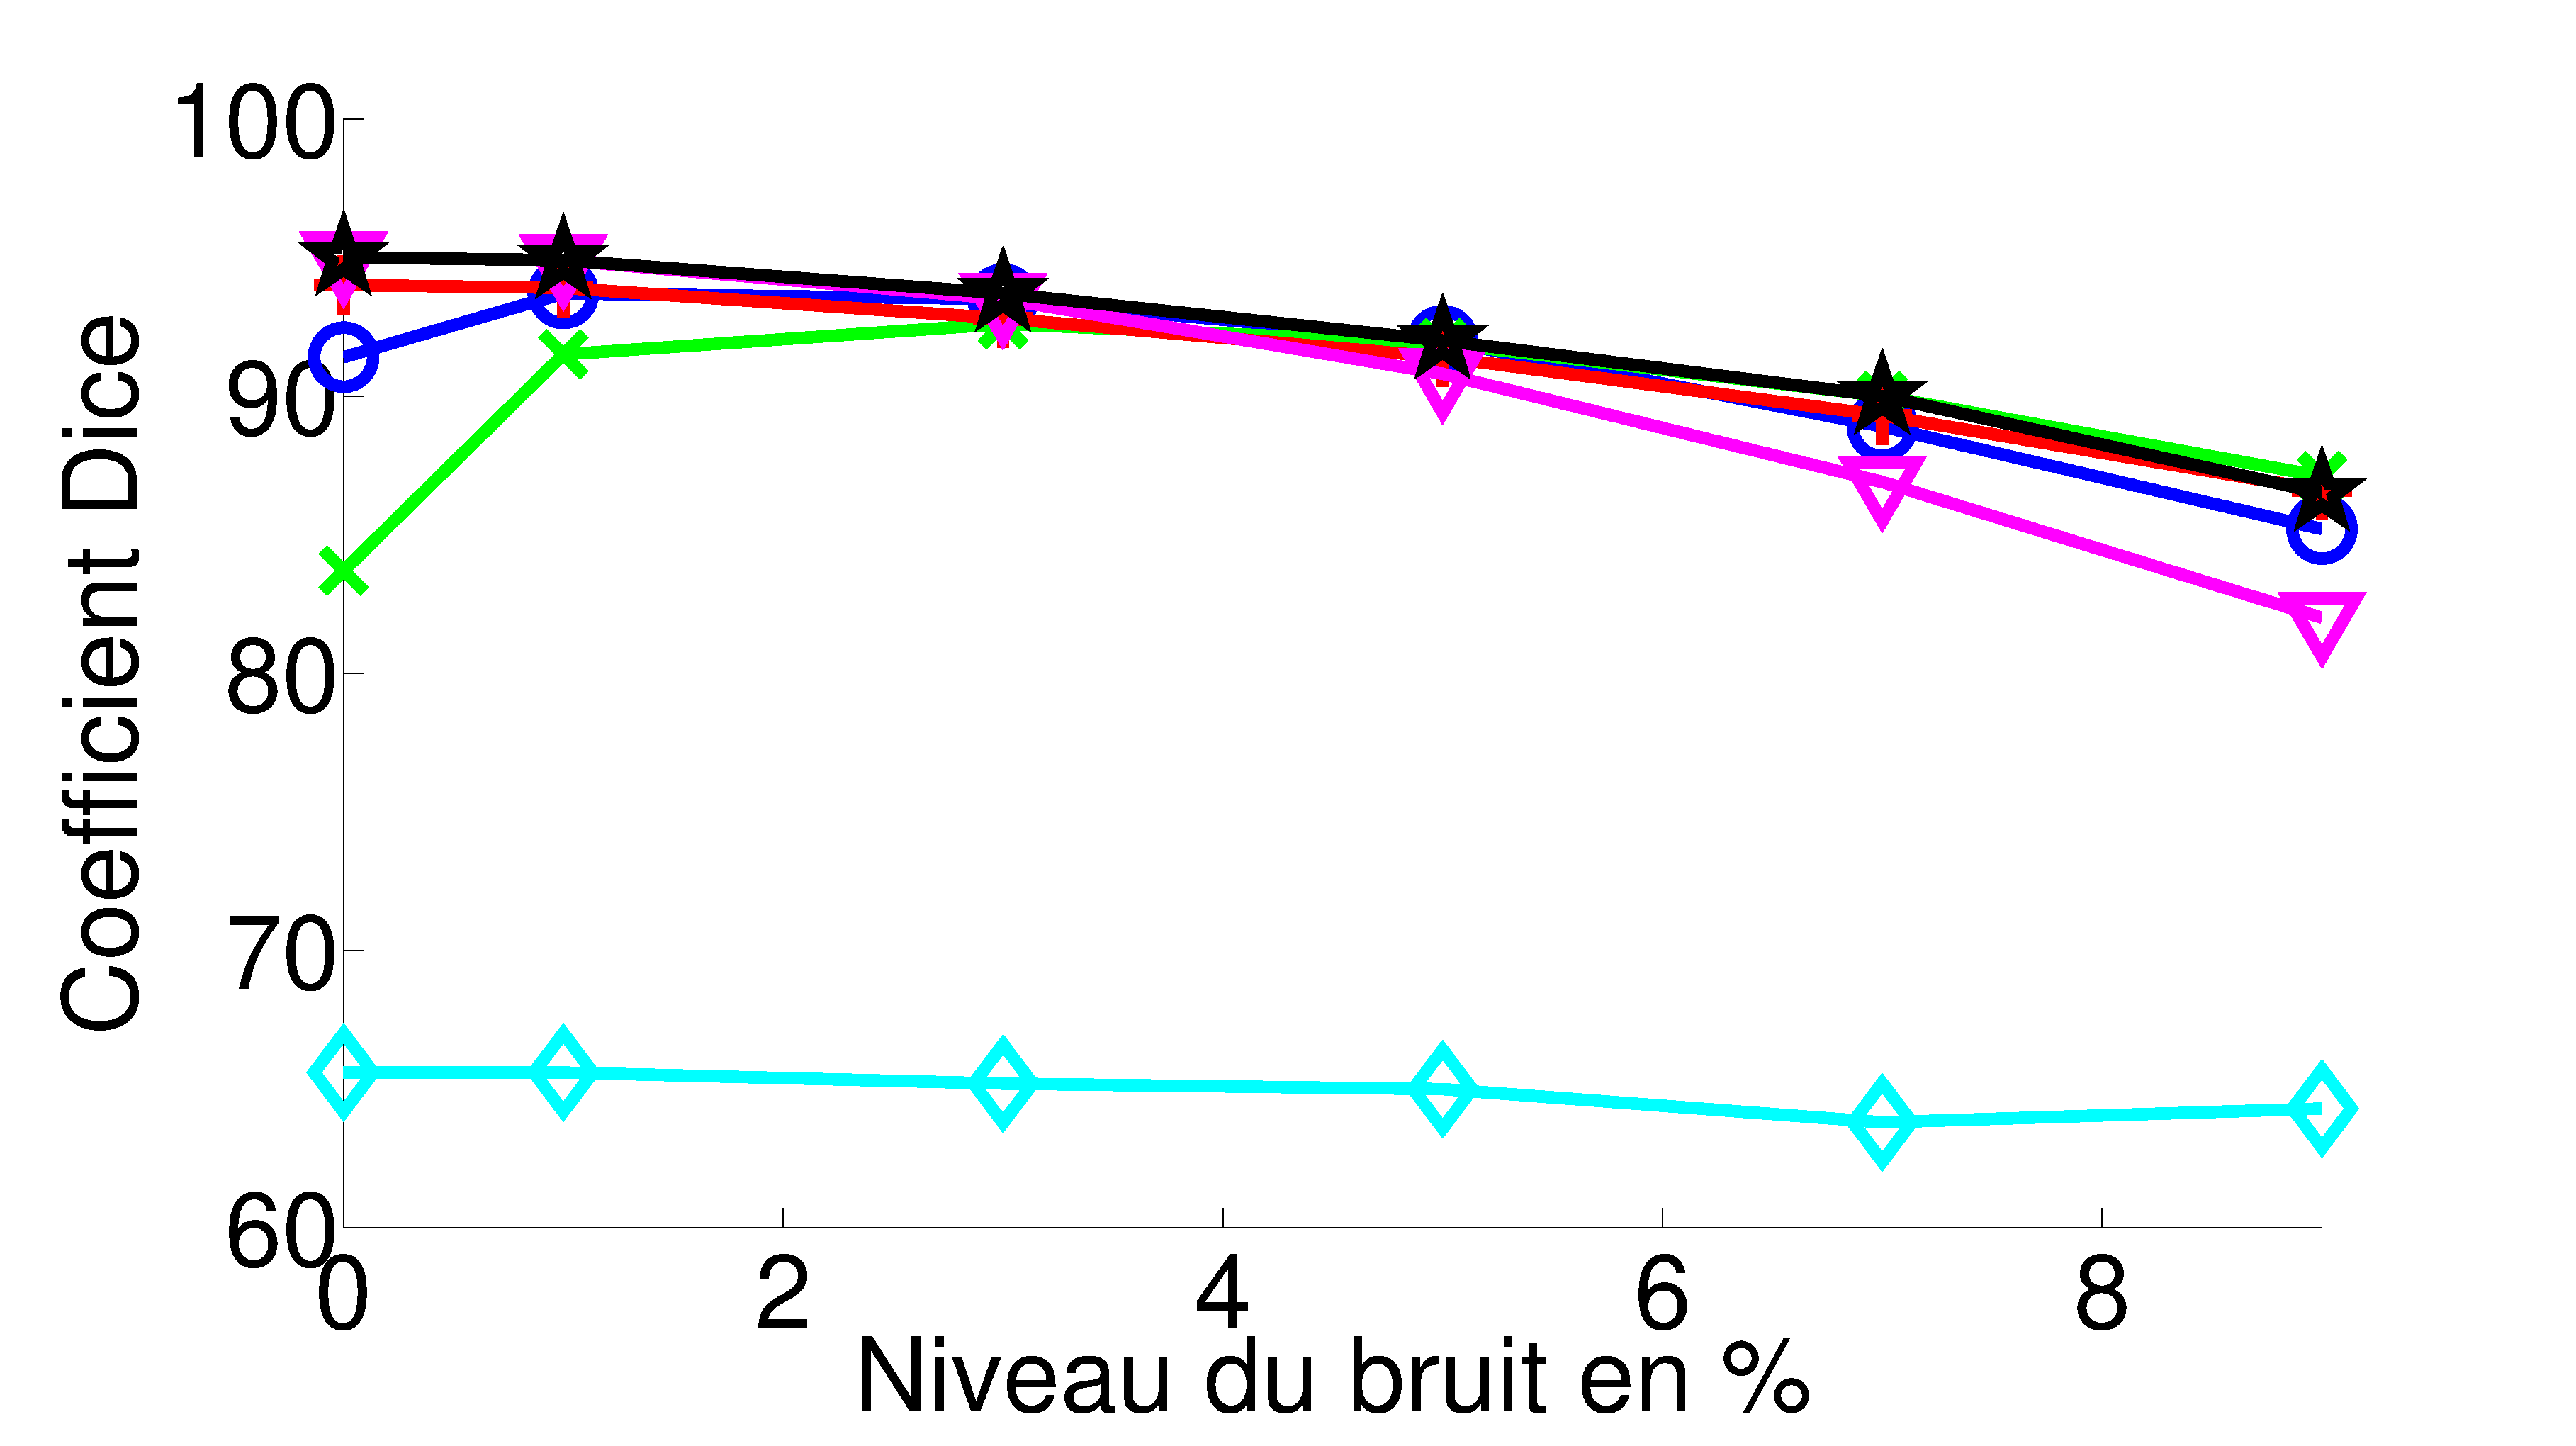
\includegraphics[height=38mm]{eps/chapitre3/Brainweb_All_GM.eps}}
	\subfigure[]{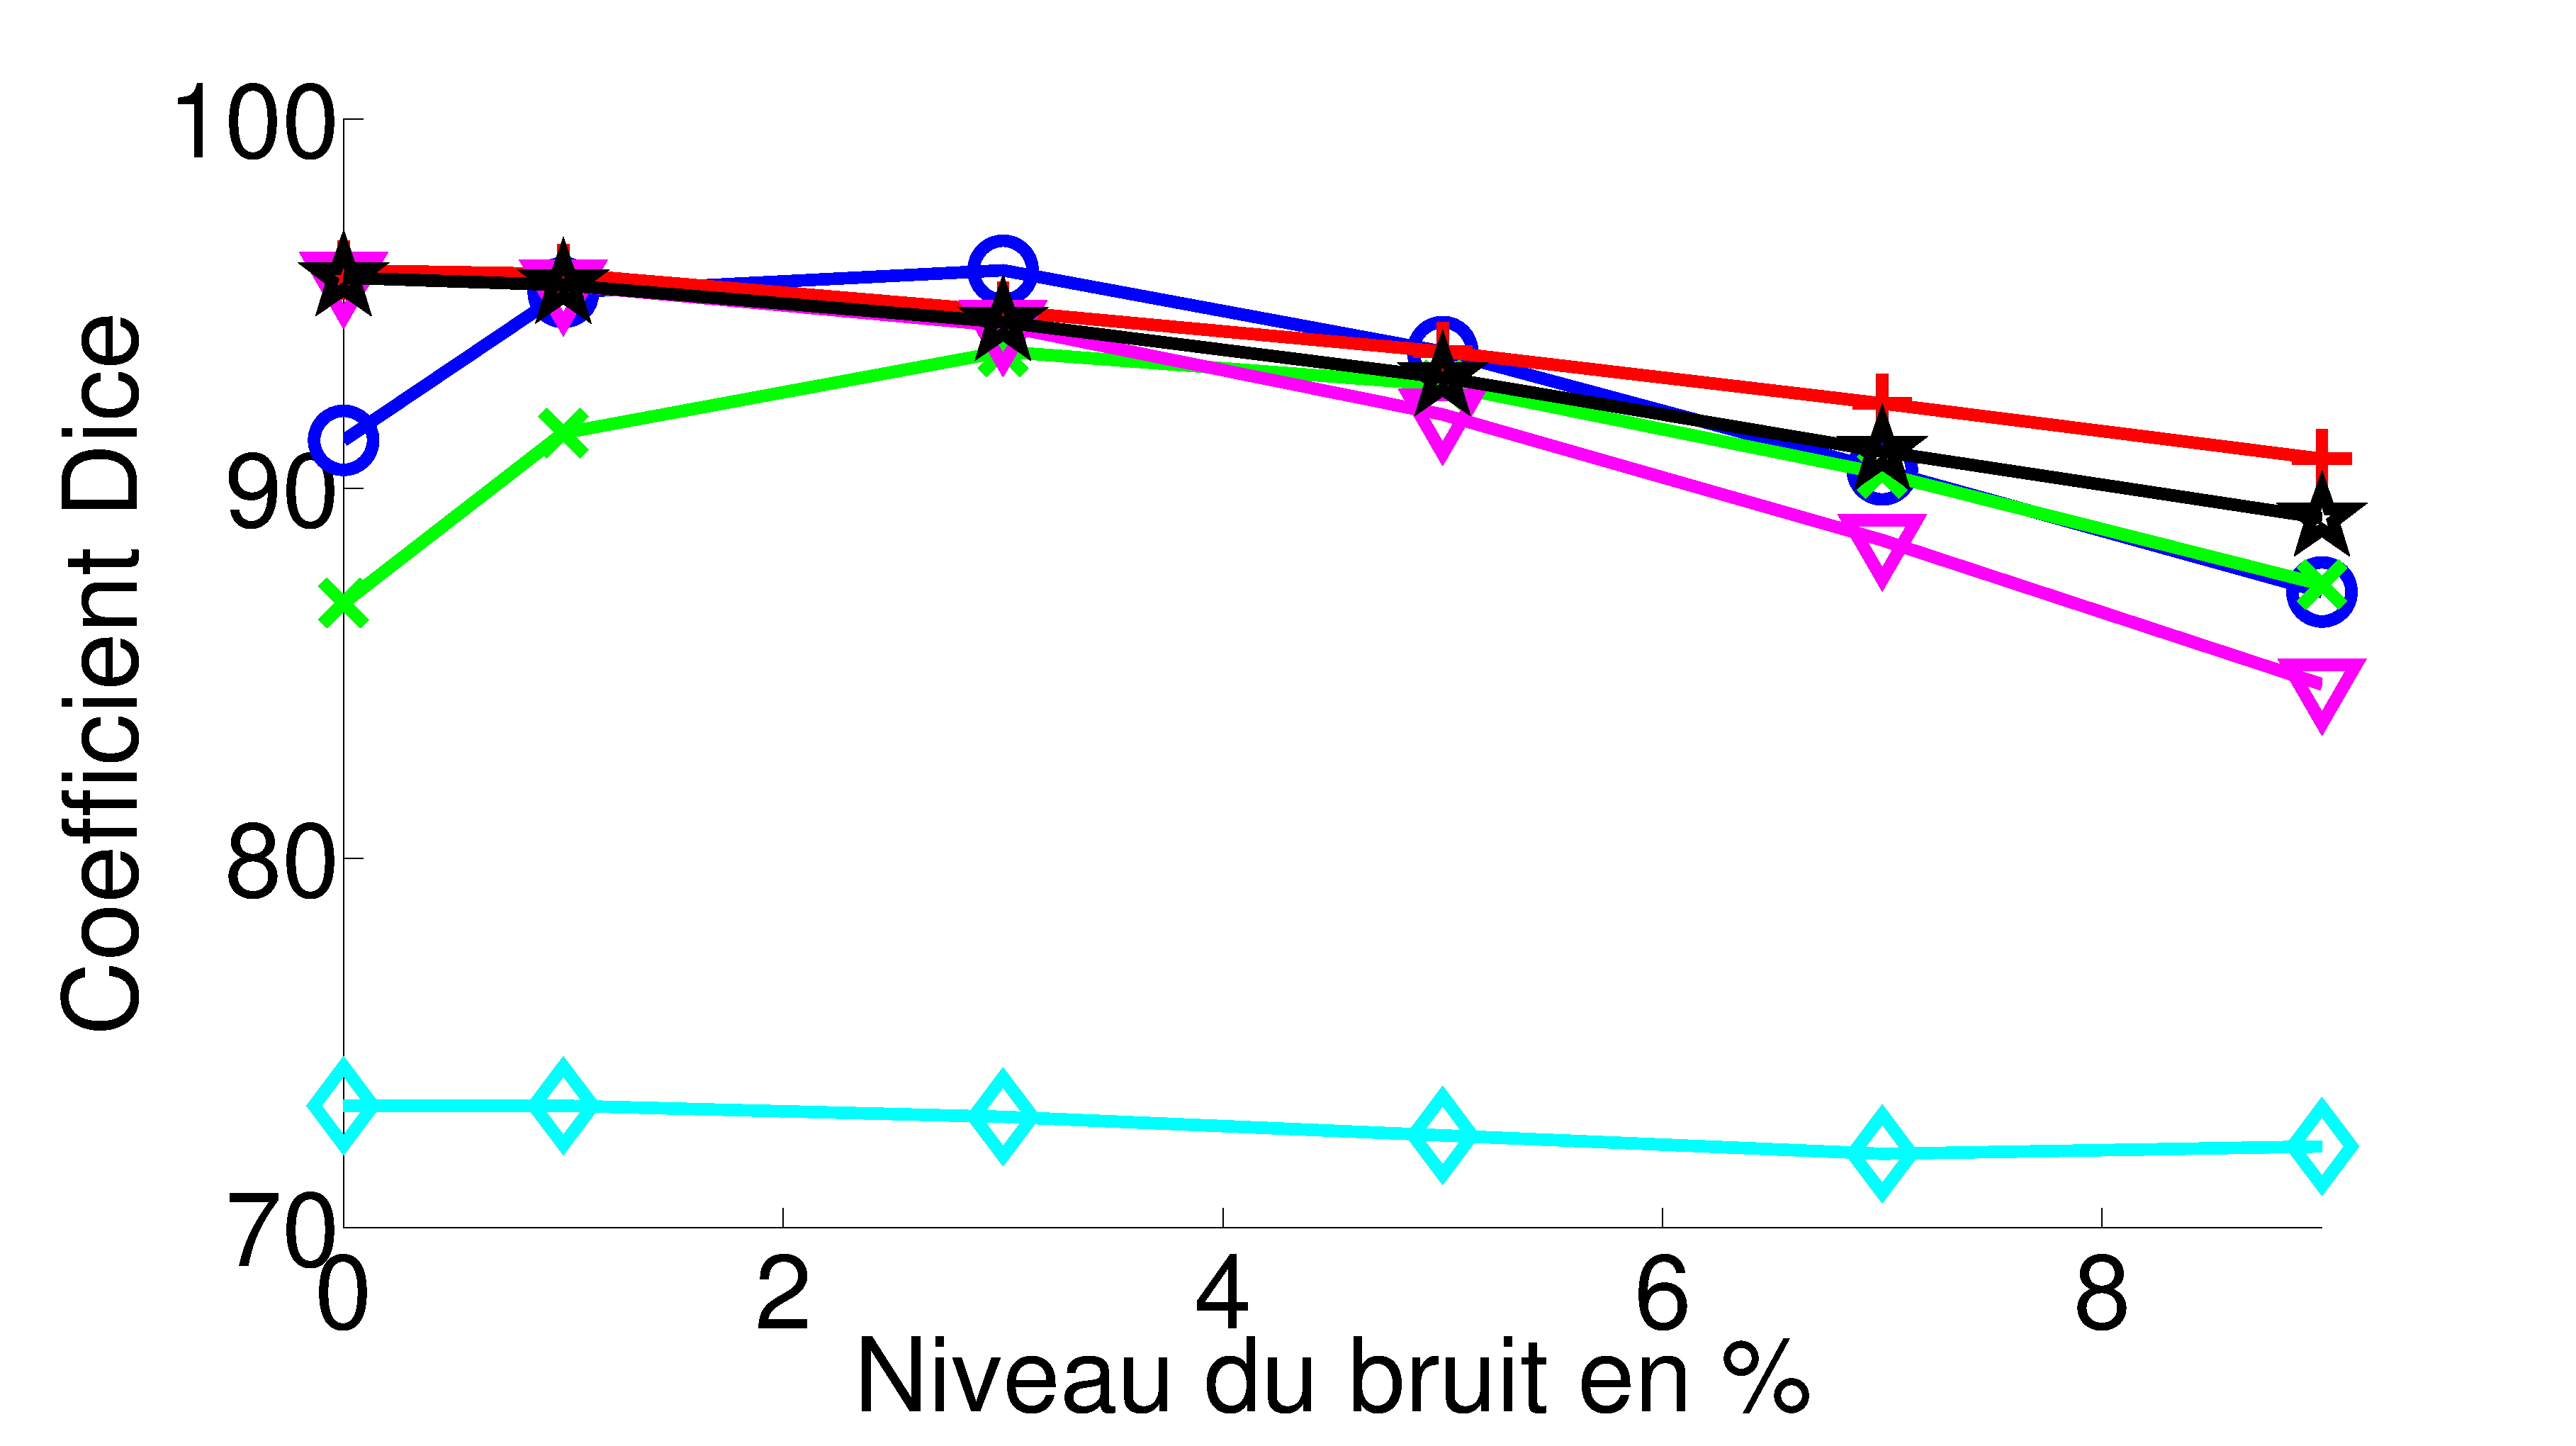
\includegraphics[height=38mm]{eps/chapitre3/Brainweb_All_WM.eps}}\\
        \end{center}

        \caption{\emph{Evolution du coefficient Dice en fonction du bruit pour différentes méthodologies. (a) Matière grise. (b) Matière blanche. Légende : SPM5 : $\circ$, EMS : $\times$, HMC : $+$, NL-Reg : $\diamond$, NL-FCM : $\bigtriangledown$, NL-R-FCM : $\star$ (Coefficients Dice pour SPM5, EMS et HMC issus de \cite{Bricq:MIA:2008}).}}

        \label{FIG:DICE:BRAINWEB:ALL}

\end{figure}

La figure~\ref{FIG:DICE:BRAINWEB:ALL} montre l'évolution des performances des différentes méthodologies avec un bruit ricien allant de $0$ à $9$~\% dans le cas de la matière blanche et de la matière grise. 
Ces deux graphiques illustrent la similarité des performances de la méthode non-locale par rapport aux algorithmes basées sur les champs et chaînes de Markov.
Une réelle différence n'est observable qu'à partir d'un niveau de bruit élevé ($7$~\%) et seulement dans le cas de la matière blanche. 
De plus, dans ce cas précis, la méthode HMC semble légèrement supérieure.

Par rapport aux résultats des sections précédentes montrant une nette amélioration de la segmentation dans le cas d'un bruit seul, ou d'un biais en intensité seul, ces résultats laissent penser que l'utilisation conjointe des deux termes non-locaux nécessite une étude plus poussée sur leur interaction de manière à déterminer une fonction d'énergie permettant une meilleure segmentation.

\subsection{IBSR}
\label{sec:ibsr}

Cette base, également disponible sur internet~\footnote{\url{http://www.cma.mgh.harvard.edu/ibsr/}}, est fournie par le Center for Morphometric Analysis du Massachussetts General Hospital.
Elle est composée de 18 volumes pondérés en T1 acquis sur des patients sains.
La taille de ces volumes est $128\times256\times256$ et chaque image dispose d'une vérité-terrain, comprenant le LCR, la matière blanche et la matière grise, réalisée par des experts.

\begin{table}[!t]
\begin{center}
\begin{tabular}{|l|c p{1.5cm}|c p{1.5cm}|}
	\hline
	Méthodes & \multicolumn{2}{|c|}{Matière Blanche (\%)} & \multicolumn{2}{|c|}{Matière Grise (\%)} \\
	& Moyenne & \centering{\'Ecart-Type} & Mean & \centering{\'Ecart-Type} \tabularnewline
	\hline
	SPM 5 \cite{Ashburner:NeuroImage:2005} & 85.27 & \centering 5.52 & 78.7 & \centering 13.98 \tabularnewline
	EMS \cite{VanLeemput2:TMI:1999} & 85.87 & \centering 2.27 & 78.94 & \centering 5.68 \tabularnewline
	HMC \cite{Bricq:MIA:2008} & 86.53 & \centering 1.73 & 79.94 & \centering 5.57 \tabularnewline
	\hline
	FCM \cite{Pham:TMI:1999} & 85.60 & \centering 3.81 & 83.21 & \centering 4.03 \tabularnewline
	R-FCM \cite{Pham:CVIU:2001} & 86.09 & \centering 2.75 & 84.08 & \centering 3.98 \tabularnewline
	\hline
	NL-Reg & 86.31 & \centering 3.18 & 83.18 & \centering 4.08 \tabularnewline
	NL-FCM & 84.68 & \centering 3.38 & 78.84 & \centering 4.07 \tabularnewline
	NL-R-FCM & 84.35 & \centering 3.38 & 83.22 & \centering 3.47 \tabularnewline
	\hline 
\end{tabular}
\vspace{2mm}
\caption{\emph{Moyennes des coefficients Dice (matière grise et matière blanche) obtenus pour différentes segmentations de la base d'image IBSR (Coefficients Dice pour SPM5, EMS et HMC issus de \cite{Bricq:MIA:2008}).\label{TAB:DICE:IBSR}}}
\end{center}
\end{table}

\begin{figure}[!thbp]

        \begin{center}
	\subfigure[]{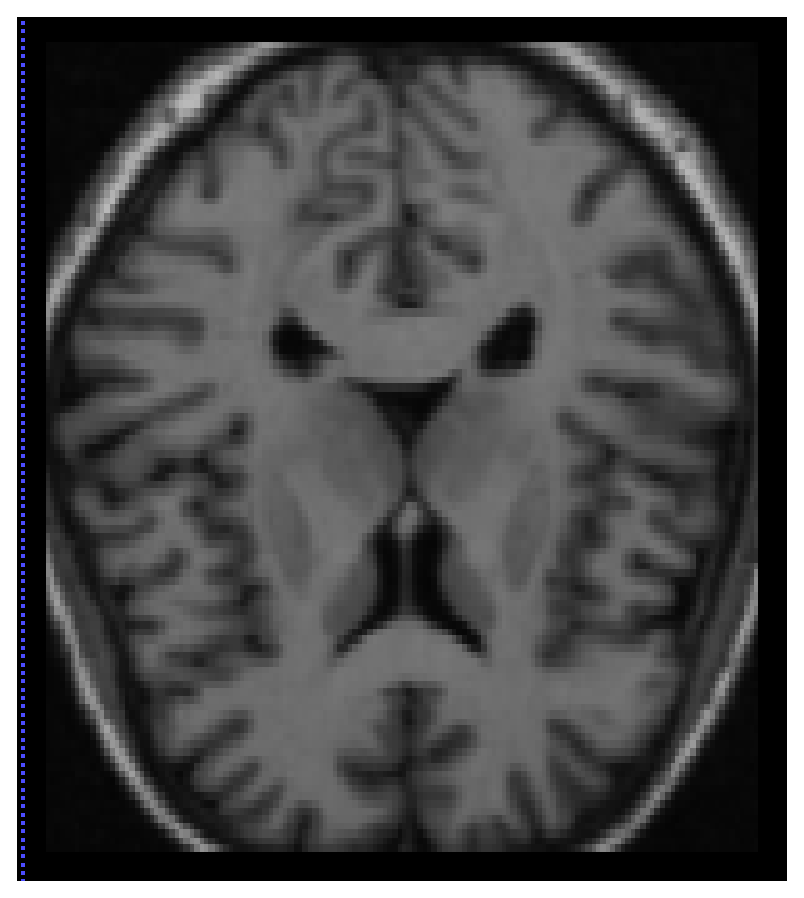
\includegraphics[height=41mm]{eps/chapitre3/IBSR_11_T1.eps}}
	\subfigure[]{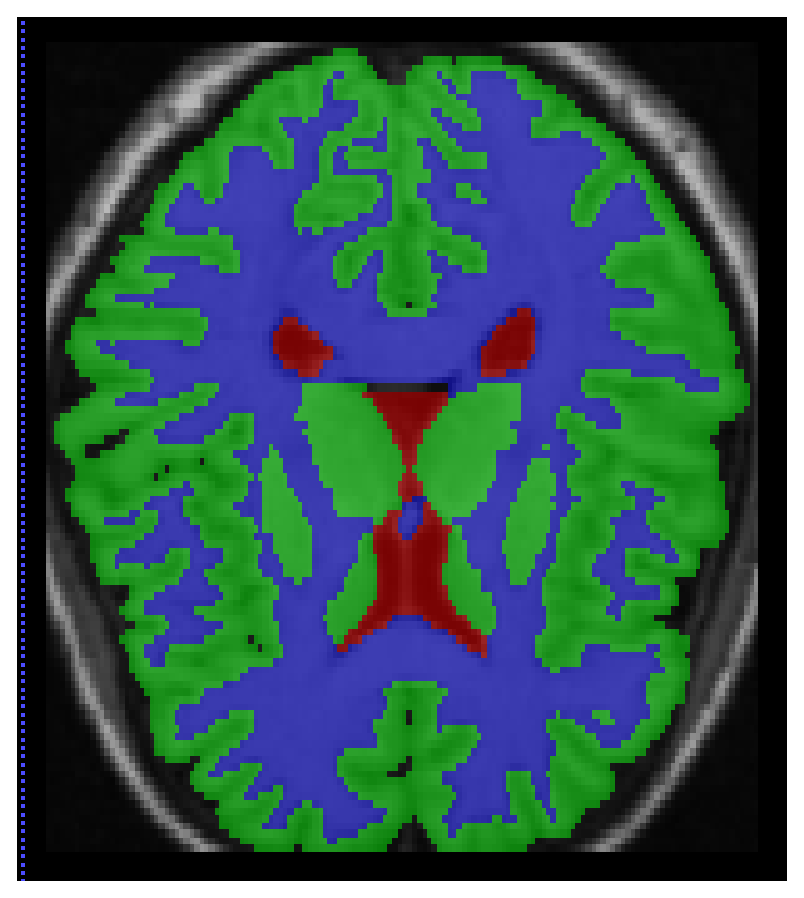
\includegraphics[height=41mm]{eps/chapitre3/IBSR_11_Truth.eps}}
	\subfigure[]{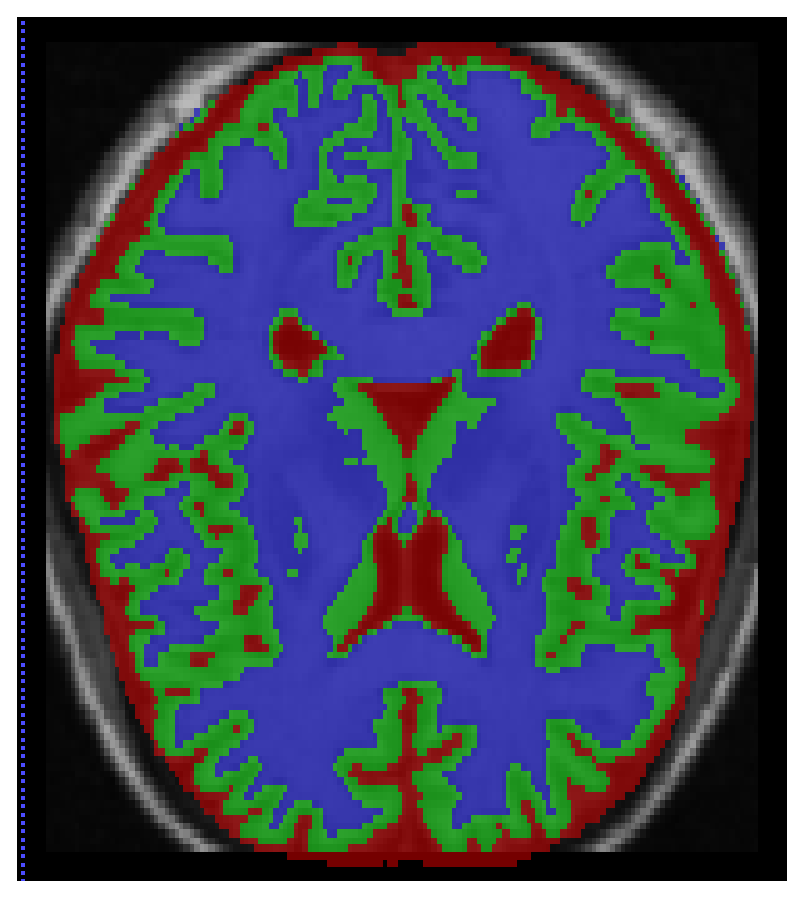
\includegraphics[height=41mm]{eps/chapitre3/IBSR_11_ClassicFCM.eps}}\\
	\subfigure[]{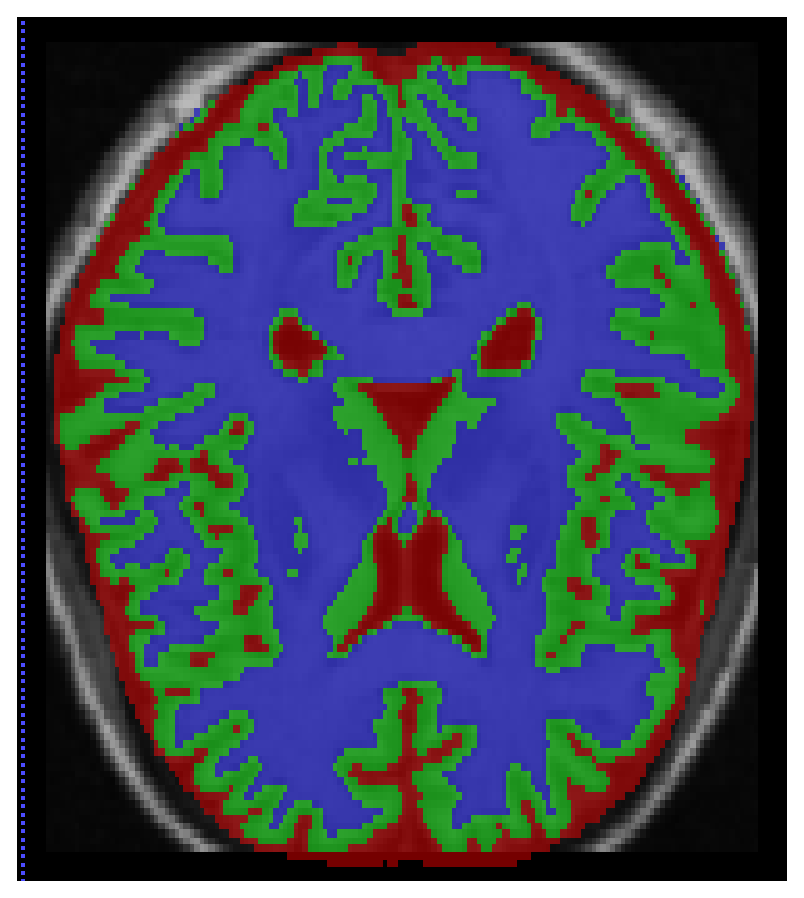
\includegraphics[height=41mm]{eps/chapitre3/IBSR_11_RFCM.eps}}
	\subfigure[]{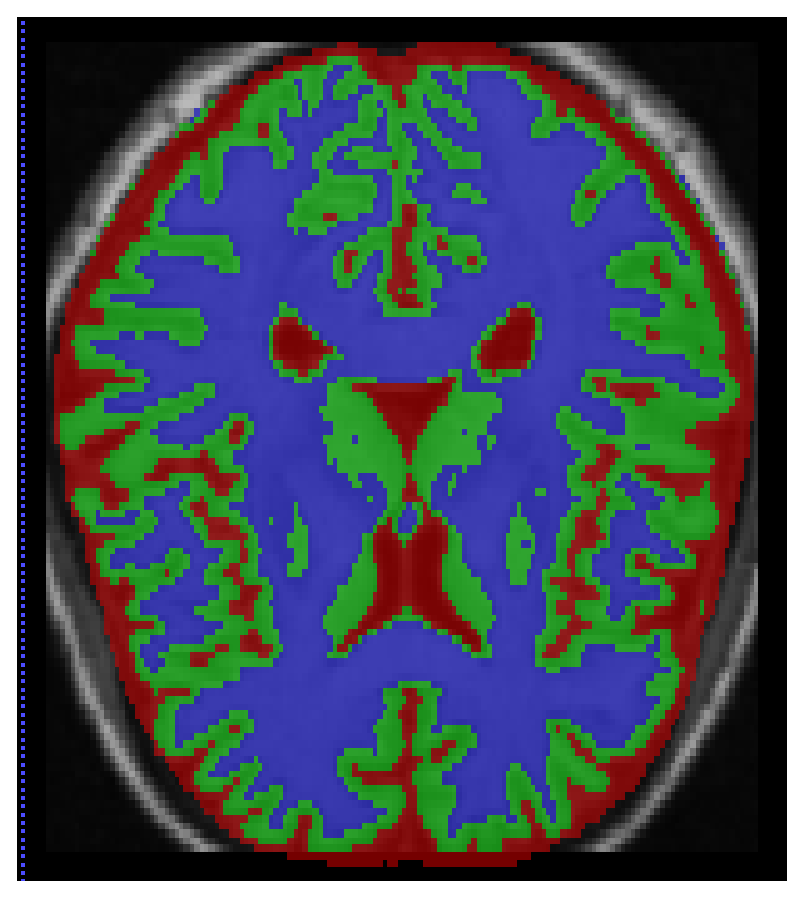
\includegraphics[height=41mm]{eps/chapitre3/IBSR_11_NLFCM.eps}}
	\subfigure[]{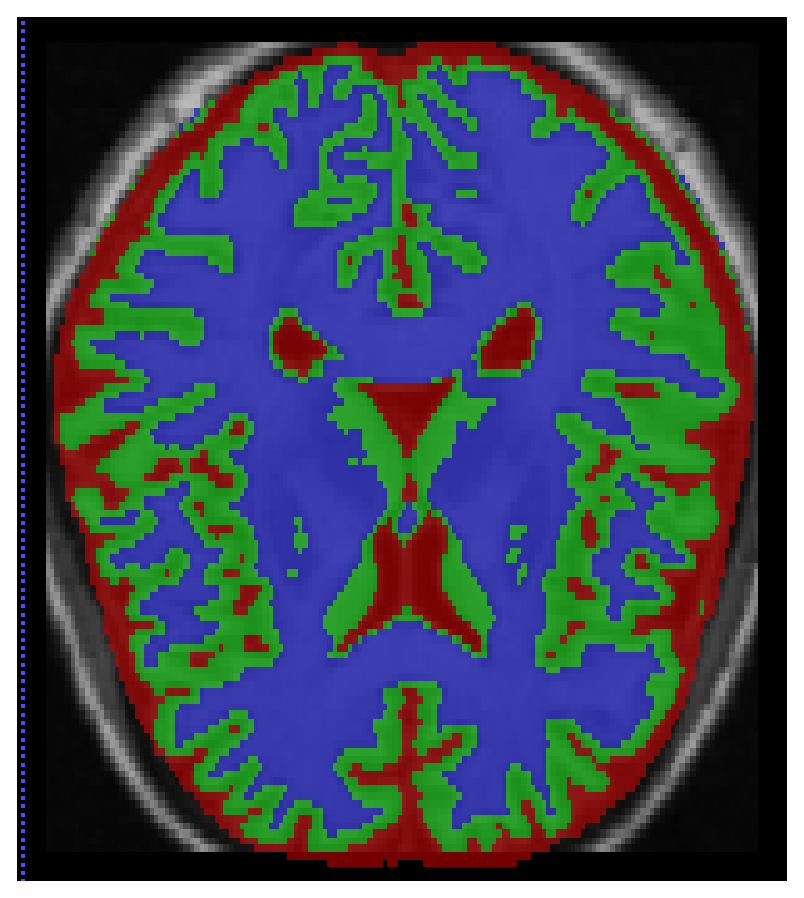
\includegraphics[height=41mm]{eps/chapitre3/IBSR_11_NLReg.eps}}
	\subfigure[]{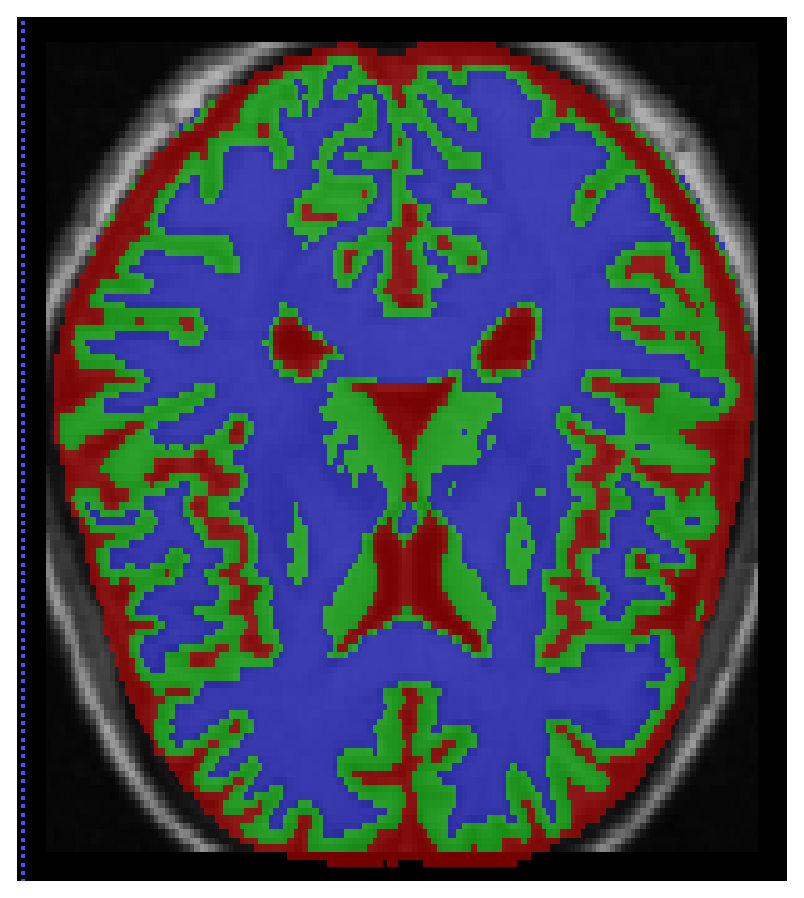
\includegraphics[height=41mm]{eps/chapitre3/IBSR_11_NLAll.eps}}
        \end{center}

        \caption{\emph{Résultats de la segmentation du cas n\textdegree11 de la base IBSR. (a) Coupe d'une image T1. (b) Vérité-terrain. (c) Segmentation par FCM classique. (d) Segmentation par RFCM. (e) Segmentation par NL-FCM. (f) Segmentation par NL-Reg. (g) Segmentation par NL-R-FCM.}}

        \label{FIG:DICE:IBSR}

\end{figure}

\begin{figure}[!thbp]

        \begin{center}
	\subfigure[]{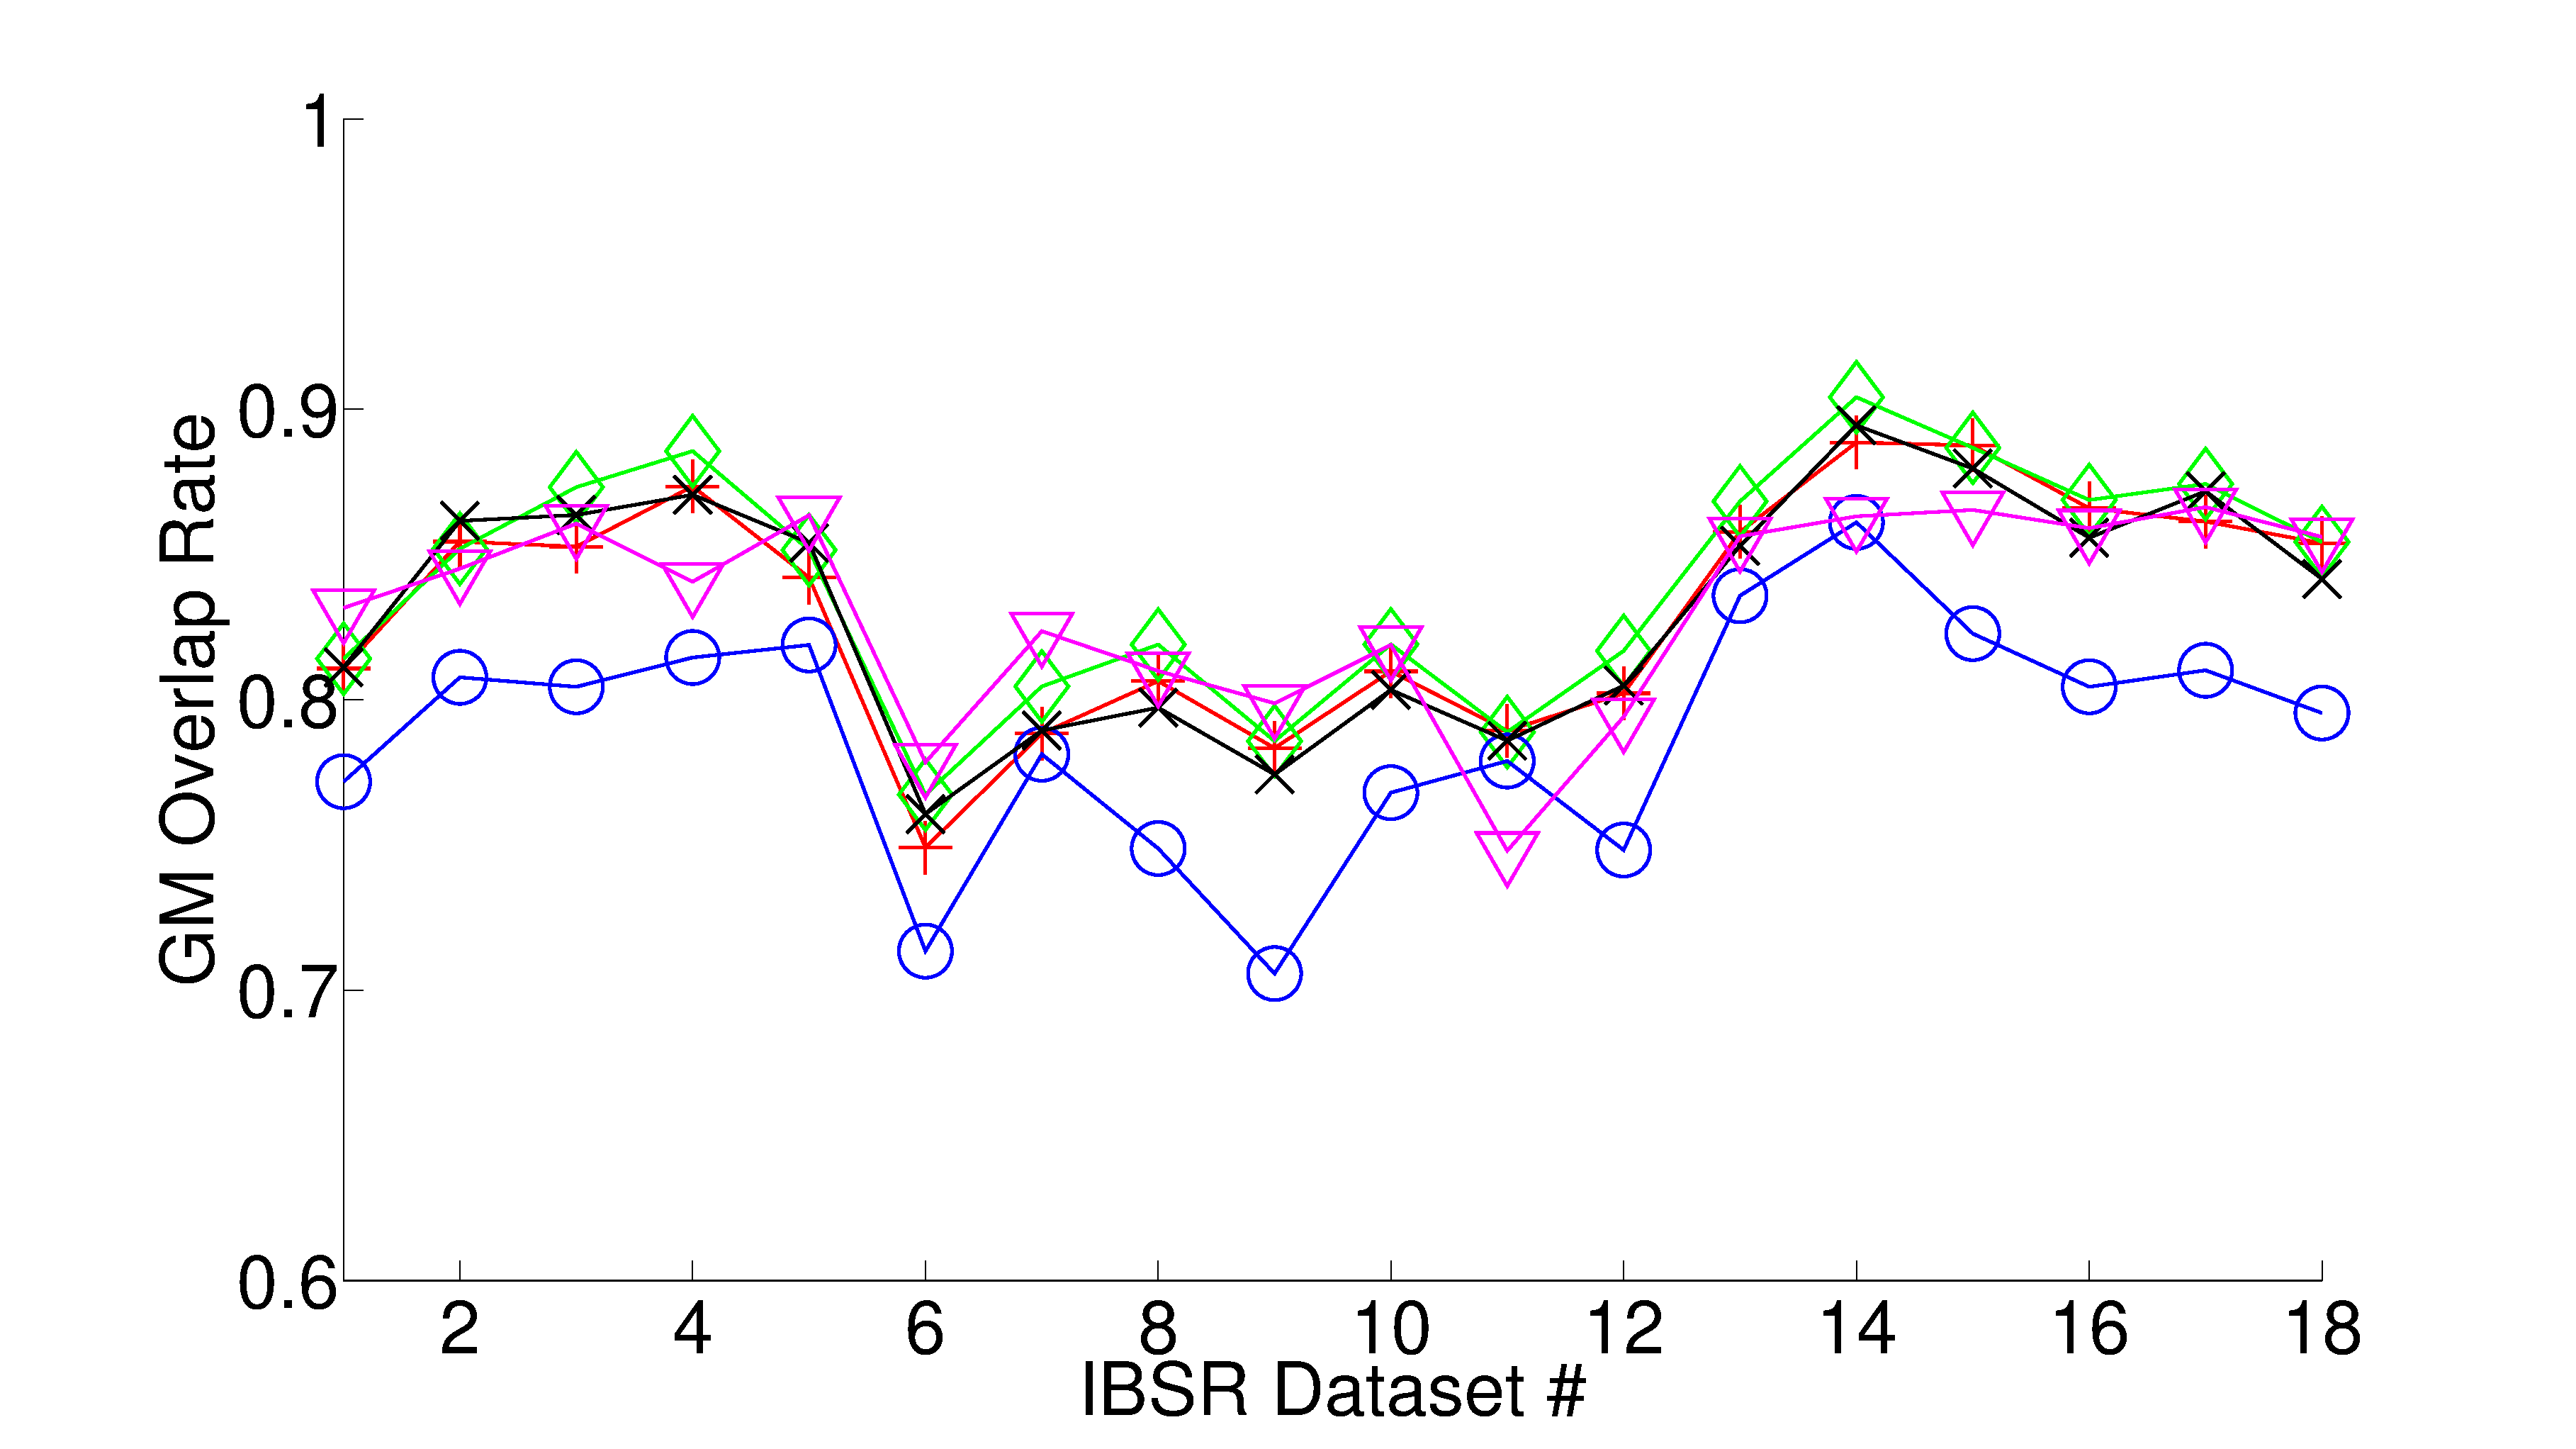
\includegraphics[height=38mm]{eps/chapitre3/IBSR_GM.eps}}
	\subfigure[]{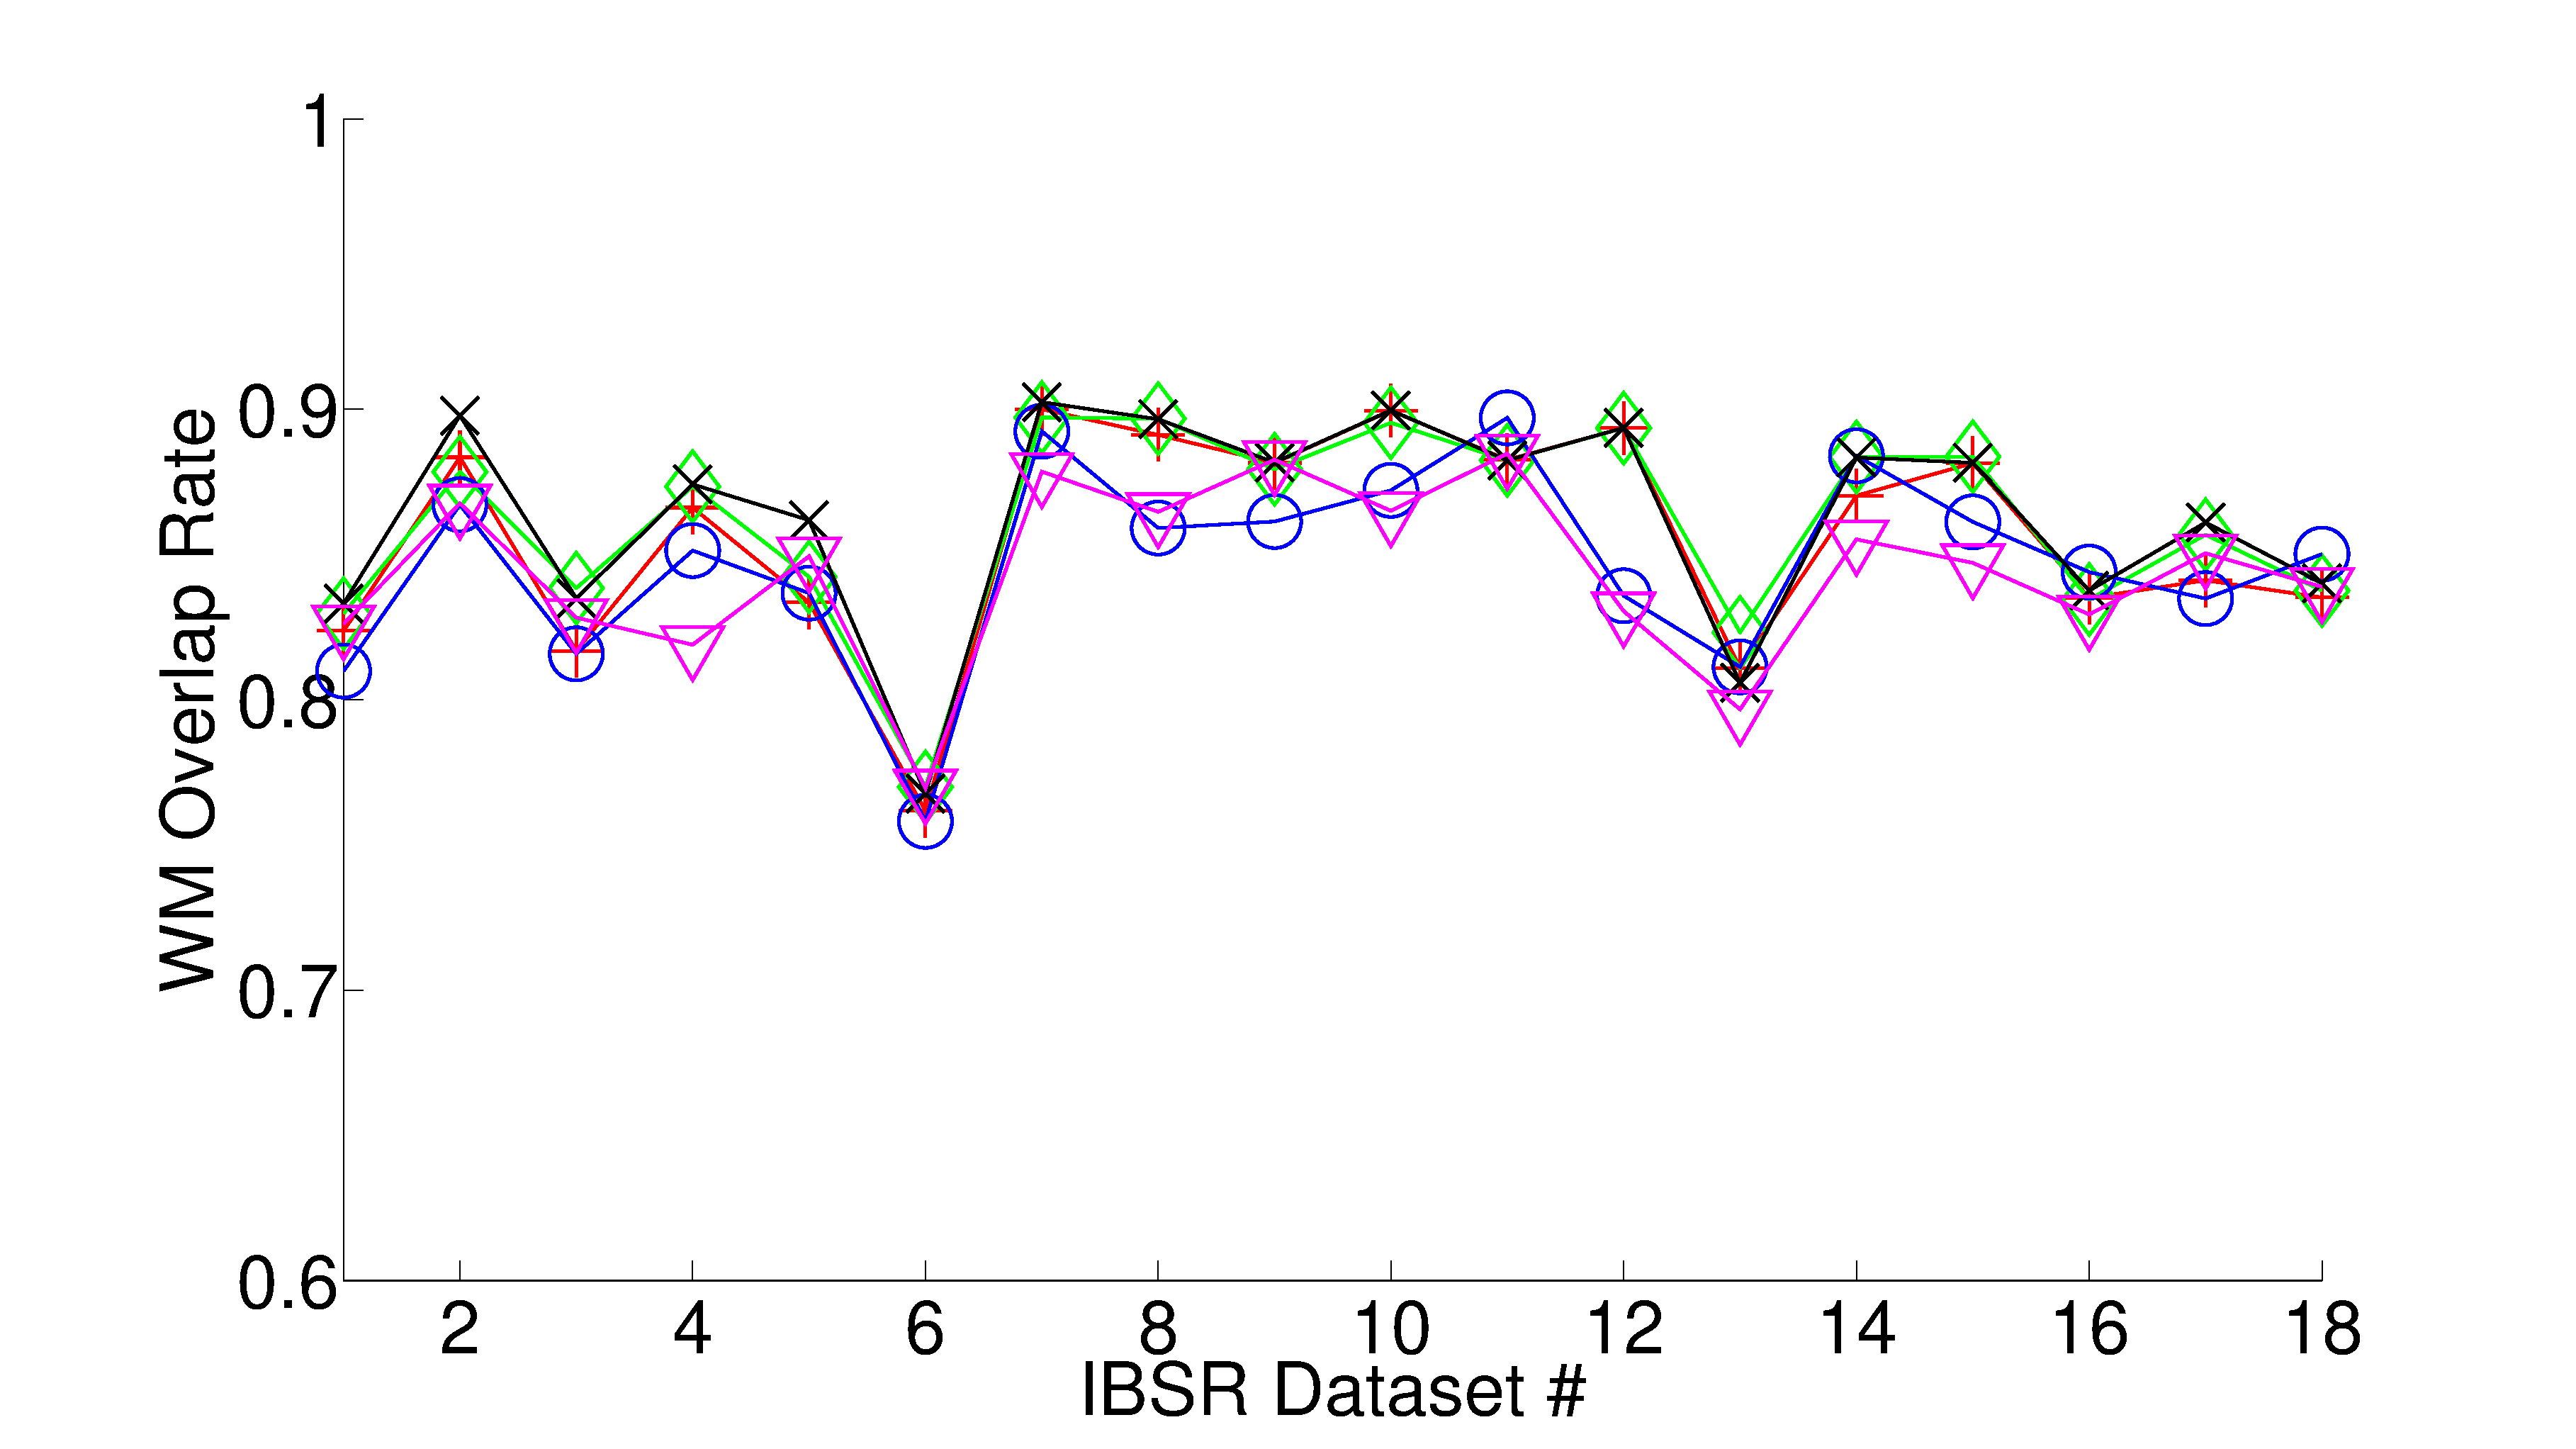
\includegraphics[height=38mm]{eps/chapitre3/IBSR_WM.eps}}
        \end{center}

        \caption{\emph{Coefficients Dice issus de la segmentation de la base IBSR. (a) Matière grise. (b) Matière blanche. Légende : FCM : $+$, RFCM : $\diamond$, NL-Reg : $\times$, NL-FCM : $\circ$, NL-R-FCM : $\bigtriangledown$}}

        \label{FIG:VIEW:IBSR}

\end{figure}

La moyenne de différentes segmentations à travers la base est calculée, ainsi que l'écart-type pour la matière blanche et la matière grise sont présentés à la table~\ref{TAB:DICE:IBSR}.
Les résultats pour chacun des cas individuels sont donnés par la figure~\ref{FIG:DICE:IBSR}.
Le LCR n'est pas considéré dans cette étude car seuls les ventricules sont segmentés manuellement.
Les résultats semblent montrer que les méthodes testées fournissent des résultats similaires, avec une meilleure efficacité des méthodes fondées sur FCM concernant la segmentation de la matière grise, aussi bien en matière de moyenne que d'écart-type.

Les résultats fournis par la figure~\ref{FIG:DICE:IBSR} montrent que les différentes méthodes basées sur FCM obtiennent des résultats similaires.
Dans les quelques cas où des résultats significativement différents peuvent être observés, par exemple le cas n\textdegree4, les meilleurs résultats sont obtenus avec les méthodes considérant des centroïdes non stationnaires.
La raison de cette homogénéité globale des résultats peut être que la plupart des cas de la base ne nécessitent pas une correction du biais, ce dernier étant très peu présent.
Ceci peut expliquer que les méthodes NL-FCM et NL-R-FCM se comportent d'une manière non-optimale car elles sont dédiées à la correction de ce biais.
Néanmoins, nous pouvons signaler que la méthode NL-R-FCM, combinant donc régularisation et correction du biais, semble fournir les résultats d'ensemble les plus stables, ce qui est illustré par des écarts-types autour de $3.5$~\% aussi bien dans le cas de la matière blanche que de la matière grise.

Il faut cependant ajouter que ces résultats doivent être interprétés avec précaution.
En effet, les segmentations manuelles fournies avec la base IBSR ne sont pas toujours optimales (par exemple autour des ventricules ou bien dans des régions très circonvoluées tels que les sillons) comme illustré à la figure~\ref{FIG:VIEW:IBSR}.
L'analyse des résultats doit donc être complétée par une observation de la segmentation des différents cas.
Elle peut être révélatrice comme dans le cas n\textdegree11 où il apparaît clairement que le matière grise est sur-segmentée, constituant ainsi un sur-ensemble de la matière grise réelle, expliquant les scores relativement plus faibles dans ce cas que dans les autres.

